\documentclass[
%	msc, %% Para dissertações de mestrado, OU
%	mscproposta, %% Para propostas de dissertação de mestrado, OU
	msc, %% Para teses de doutorado, OU
%	phdproposta, %% Para propostas de tese de doutorado
	portugues %% Para documentos em português, OU
%english %% Para documentos em inglês
]{../ppgccufmg}

\usepackage[brazil]{babel} %% se o documento for em português, OU
%\usepackage[english]{babel} %% se o documento for em inglês
%\usepackage[latin1]{inputenc}
\usepackage{xcolor}
\usepackage{natbib}
\usepackage{csvsimple}
%\usepackage{xcolor}[table]
\usepackage{booktabs}
\usepackage{adjustbox}
\usepackage{graphicx}
\usepackage{subcaption}
\usepackage{lipsum}
\usepackage{multirow}
\usepackage{graphicx}
\usepackage{colortbl}
\usepackage{array}
\usepackage[
	colorlinks=true,
	linkcolor=blue, %% Cor dos links do sumário
	citecolor=red, %% Cor dos links das citações
	urlcolor=magenta, %% Cor das urls
]{hyperref}

\newfloat[chapter]{algoritmo}{lol}{Algoritmo}
\newcommand{\listaalgoritmosname}{Lista de Algoritmos} %% Título da lista
\newlistof{listadealgoritmos}{lol}{\listaalgoritmosname} %% O primeiro parâmetro é o nome da lista, e este deverá ser passado no parâmetro listacustomizada={\nomedalista}
\newlistentry{algoritmo}{lol}{0} %% Nome do ambiente de cada algoritmo, e.g., \begin{algoritmo} ... \end{algoritmo}

%% **** Caso não haja nenhuma lista adicional, os comandos acima podem ser apagados. ****
%% ===============================================

\begin{document}
	\ppgccufmg{
		autor={Felipe Glicério Gomes Marcelino}, %% Autor(a)
		titulo={Deteção de Glaucoma Através de Aprendizado de Máquina}, %% Título
		cidade={Belo Horizonte},
		ano={2022},
		versao={Final}, %% Versão do documento
		orientador={Adriano Alonso Veloso}, %% Para masculino
		%orientadora={Fulana de Tal}, %% Para feminino
%		coorientador={Ciclano}, %% Para masculino
		%coorientadora={Ciclana}, %% Para feminino
		fichacatalografica={fichacatalografica.pdf},
		folhadeaprovacao={folhadeaprovacao.pdf},
		resumo={resumo.tex}, %% Resumo em português
		abstracten={abstract.tex}, %% Abstract em inglês
		palavraschave={Aprendizao de Máquine. Computação Visual. Modelagem. Glaucoma. Diagnóstico.
        Explicabilidade.}, %% Palavras-chave do resumo
		keywords={Machine Learning. Computer Vision. Modeling. Glaucoma. Diagnostic. Explainability}, %% Palavras-chave do abstract
		dedicatoria={dedicatoria.tex}, %% Arquivo .tex contendo a dedicatória
		agradecimentos={agradecimentos.tex},
		epigrafe={},
		epigrafeautor={},
		listadefiguras={sim}, %% Remova (ou comente) este parâmetro para remover a lista de figuras
		listadetabelas={sim}, %% Remova (ou comente) este parâmetro para remover a lista de tabelas
		listascustomizadas={\listadealgoritmos} %% Lista customizada (e.g., lista de algoritmos).
	}

	\chapter{Introdução}\label{intro}
        Glaucoma é uma doença neuropática progressiva que resulta na mudanças de caracteŕisticas do
        disco ótico e causa danos irreversíveis nas fibras nervosas \citep{felipemedeiros2014}. Apesar de ser irreversível, é
        possível que com tratamente a evolução da doença seja mais lenta
        \citep{GARWAYHEATH201368}. Uma das formas de
        diagnóstico do glaucoma é feito através de imagens que requer análise e interpretação de um especialista da
        área. Dado que o número de pessoas com a doença aumentará em 111,8 milhões até 2040
        \citep{Ottaiano2019}, métodos utilizando inteligência artificial vem sendo utilizados para
        automatizar o processo \citep{Barros2020}.


        Um dos grandes desafios quanto ao diagnóstico do glaucoma são os aspectos assintomáticos da
        doença antes dos estágios severos. Dado isso, o número de pessoas não diagnósticadas
            corretamente é grande \citep{burgoyne}. Atualmente,
            um dos recursos mais utlizados para detectar a doença é a imagem da retina ou imagem do
            fundo do olho. Com a imagem do fundo do olho é possível verificar o
            o formato e o tamanho do disco óptico, já que este sofre alterações na presenca da
            doença \citep{zangali}. Algoritmos de aprendizado por máquina
        (\textit{machine learning}) são utilizados juntos com imagens de retinas para identificar a
        doença. Estes algoritmos podem utilizar técnicas de aprendizado estatisticos ou aprendizado
        profundo \citep{Barros2020}.

        Aprendizado de máquina vem se tornando um dos desenvolvimentos mais importantes no campo de
        ciência e tecnologia, principalmente na medicina. Classificação é uma das principais
        técnicas de aprendizado de máquina utilizado no campo médico. Isto porque porque utilizando
        modelos classificadores é possível prever diagnósticos de doenças utilizando dados médicos clínicos
        e exames de imagens. Desta forma, classificação se torna uma técnica inerente para detecção de
        glaucoma. No futuro, aprendizado de máquina será essencial não somente para diagnosticar mas
        também para tratar o glaucoma.

        O fundoscopia do olho possibilita que especialista consiga identificar todas as
        estruturas oculares necessárias para identificaro glaucoma, como por exemplo: disco óptico
        (DO), copo óptico (CO), mácula lútea, fóvea e os vasos sanguíneos \citep{SON202085,
        albander201891,ZHU201768}. As maiores vantagens de se utilizar a imagem do fundo do olho são: Não é
        um processo invaso, é seguro e ajuda na detecção de outras doenças.

        O exame OCT para glaucoma é também indicado para diagnósticar e dar suporte na evolução dos tratamentos (médicos ou cirurgia).
        O OCT permite estudar a espessura da camada de fibras nervosas da retina peri-papilares assim como a escavação do disco ótico.
        Existem diferentes aparelhos de OCT, que apresentam variadas velocidades e definições de
        imagem. De qualquer forma, o OCT fornece medições da espessura da fibras em diferentes
        regiões retina. Estas medições forcenem aos profissiona um grande número de informações,
        dando mais recurso para uma melhor avaliação do glaucoma.


        \begin{figure}
            \centering
            \caption{Exemplos de imagem do fundo do olho com presença e ausência de glaucoma.}
            \label{glaucomadiff}
            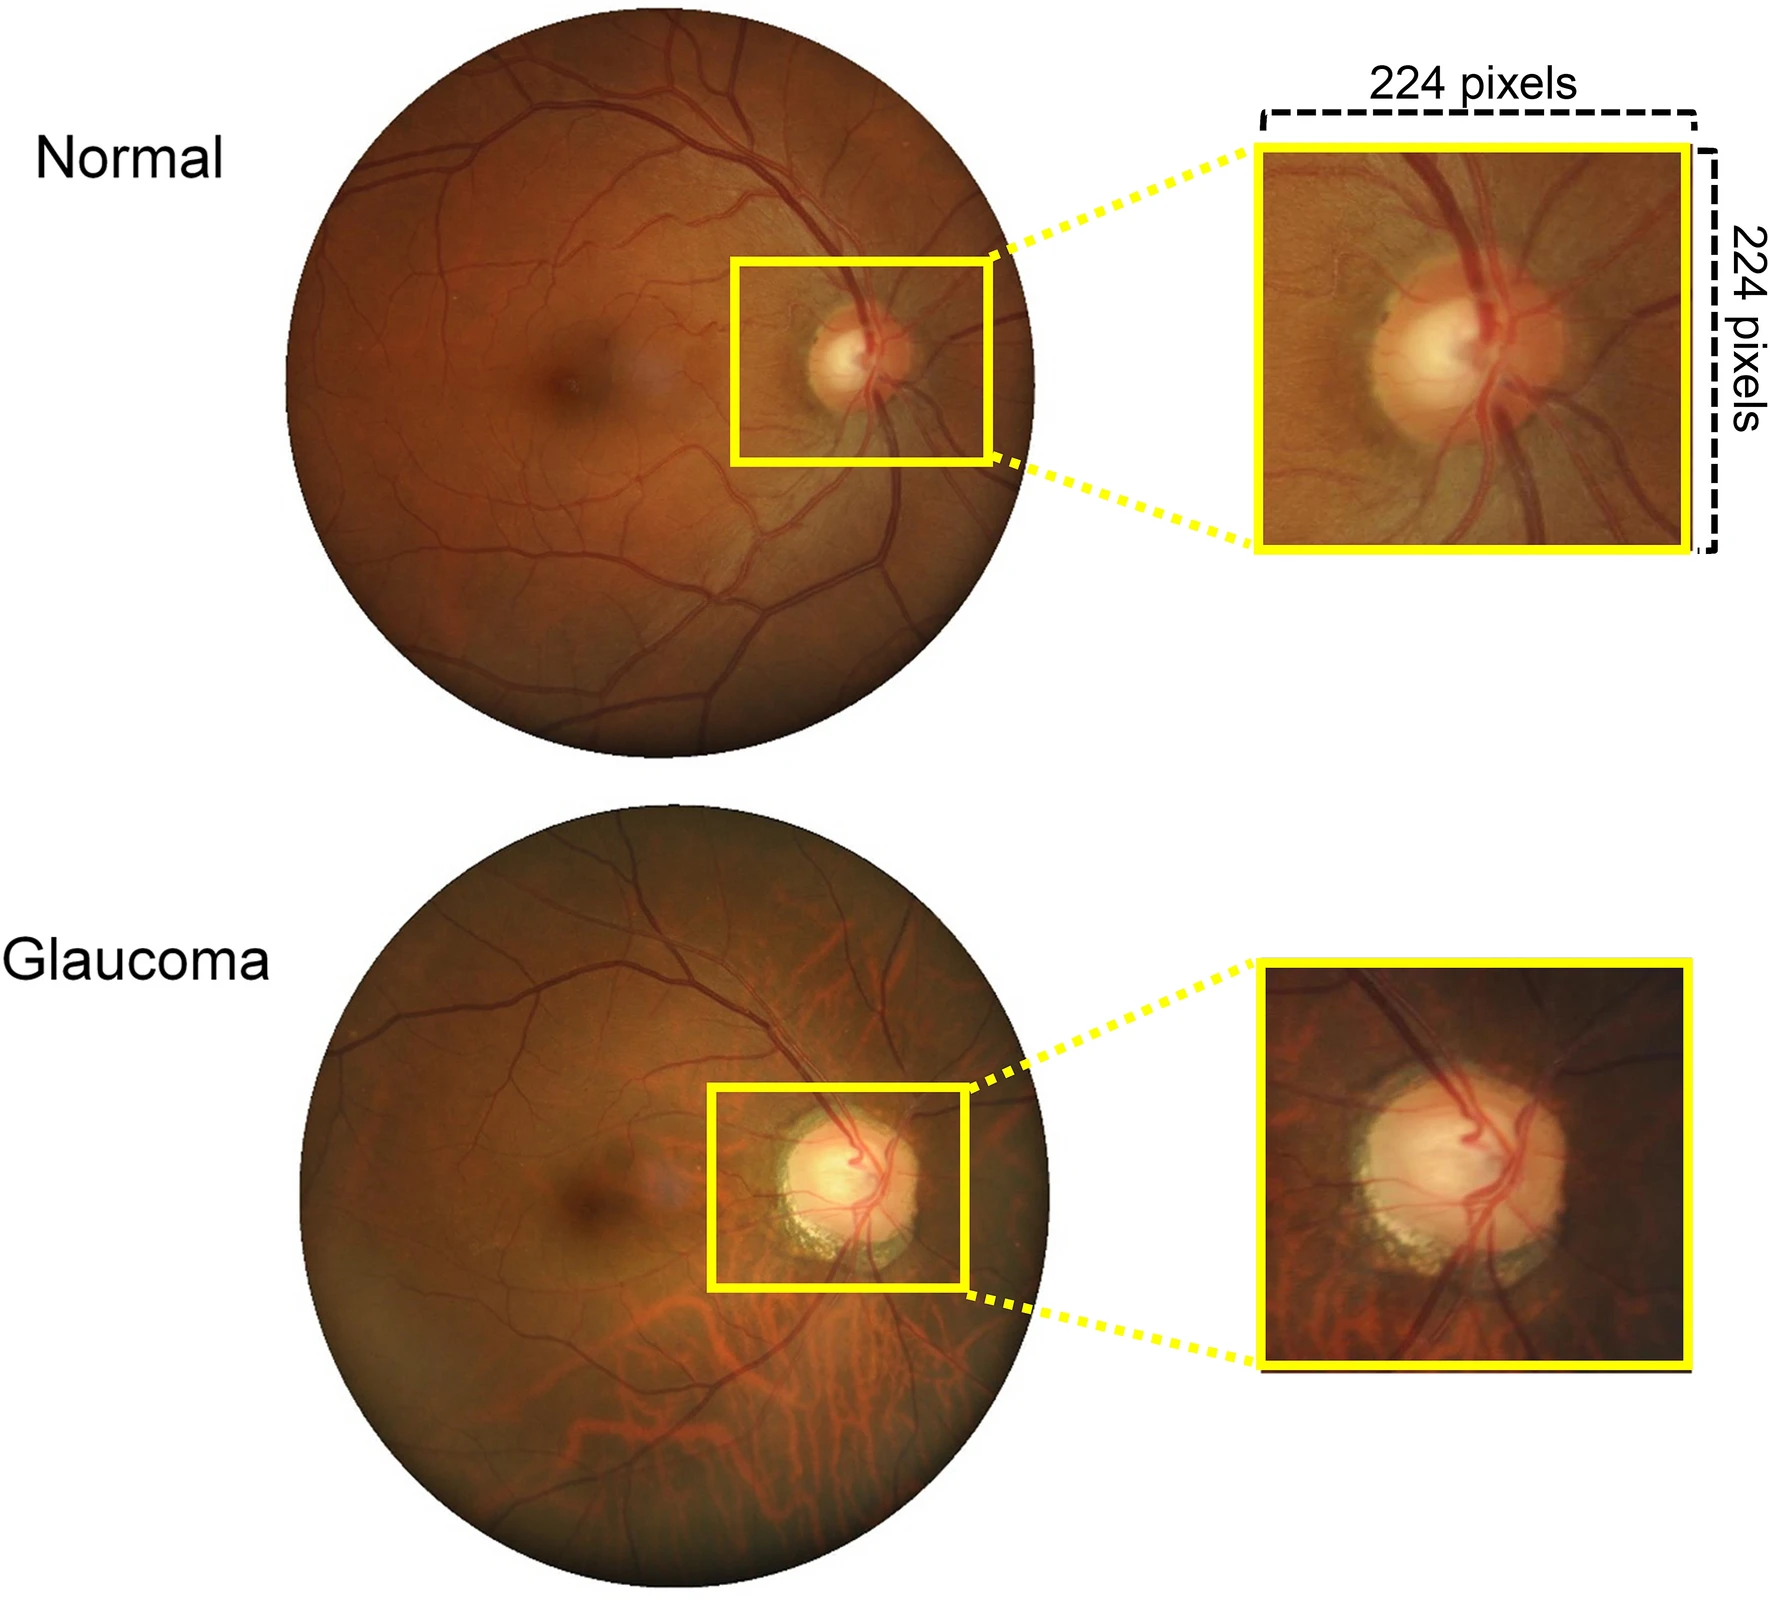
\includegraphics[width=0.6\textwidth]{./img/glaucoma_diff.png}
            \small{Fonte:
            \href{https://www.nature.com/articles/s41598-021-81554-4}{Nature, 2021}}
        \end{figure}

        A fígura~\ref{glaucomadiff} traz duas imagens de fundo de olho para compararmos o caso em
        que há presença de glaucoma. É possível ver na segunda imagem do fundo do olho o aumento da
        proporção entre o copo óptico e o disco óptico (\textit{cup-to-disc}).

        \begin{figure}
            \centering
            \caption{Exemplo de exame OCT, sendo o olho direito (OD) com a presença de glaucoma e o
            esquerdo(OS) em estado saudável}
            \label{octdiff}
            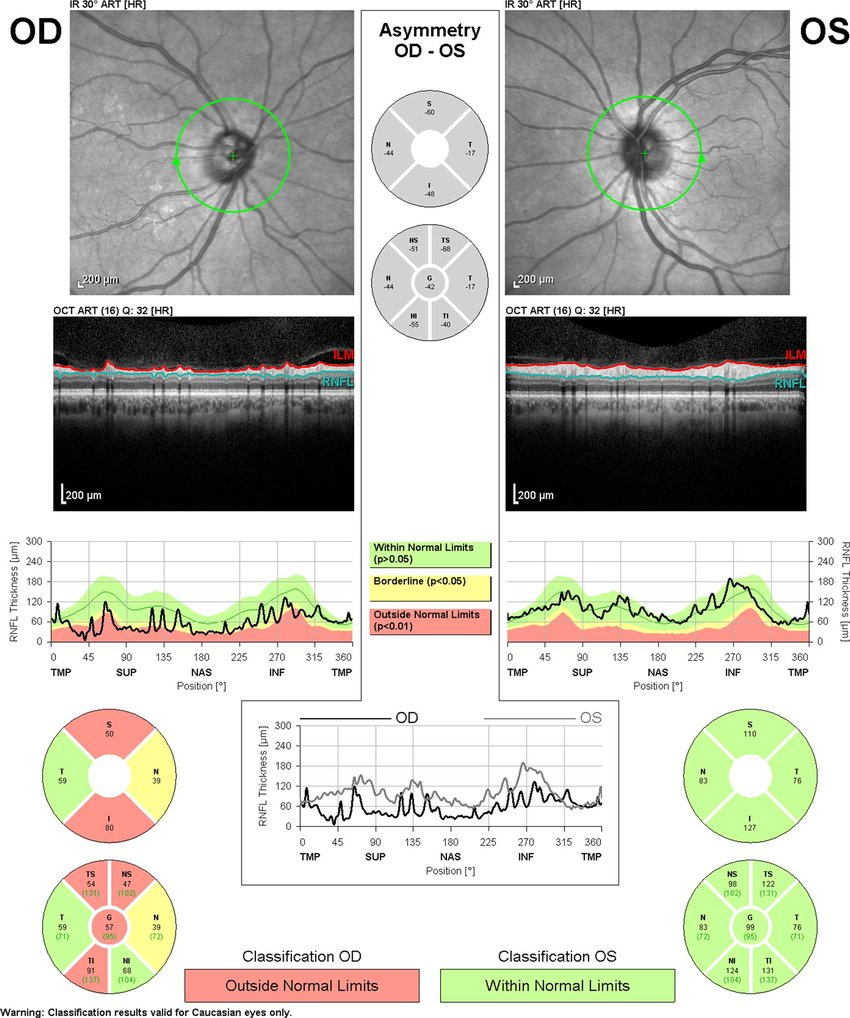
\includegraphics[width=0.6\textwidth]{./img/oct.jpg}
            \small{Fonte:
            \href{https://glaucomatoday.com/articles/2016-may-june/optical-coherence-tomography-as-a-glaucoma-screening-tool}{Glaucoma
            Today, 2016}}
        \end{figure}

        A fígura~\ref{octdiff} mostra um exame OCT com suas respectivas medidas de espessura das
        fibras da retina. A espessura da fibras em dividido em 6 setores: nasal (N), nasal super (NS),
        nasal inferior (NI), temporal (T), temporal superior (TS), temporal inferior (TI). Além disso,
        temos o valor G que é média dos quadrantes dos setores. Dado isso, quanto menor o valor G
        maior a probabilidade de se ter glaucoma. A fígura~\ref{octdiff} nos mostra que o olho
        direito está com as fibras danificadas, com possibilidade de glaucoma, enquanto o olho esquerdo apresenta um estado
        saudável.

        Dado as caraterísticas citadas acimas, a imagem do fundo do olho e OCT são primordialmente
        utilizados por sistemas inteligentes. Tais sistemas, utilizando exames médicos, são capazes
        de trazer um diagnóstico e uma segunda opinião, dando suporte ao profissional da saúde.
        Sistemas inteligentes de diagnósticos são capazes de provê interpreatações clínicas para
        auxiliar o profissional nas decisões de tratamento e diminuir as chances de ações
        prejudiciais ao paciente \citep{HAGIWARA20181,SCHMIDTERFURTH20181}.


        \section{Aprendizado de máquina aplicado a diagnósticos com imagens}

        O desenvolvimento novas tecnológias envolvendo aprendizado de máquina vem mostrando grandes
        avanços, principalmente no campo médico. O envolvimento da inteligência artificial (IA) em outros
        campos, fez com que as aplicações de aprendizado de máquina seja interdisciplinar,
        adentrando soluções que envolve reconhecimento de voz, reconhecimento de objetos, predição
        de demanda, veículos autônomos e etc. Para a aŕea médica, além do diagnóstico, é possível
        utilizar IA para descobrir novas drogas, melhorar a comunição entre médico e paciente,
        transcrever documentos médicos, como por exemplo receita e também tratamento remoto dos
        pacientes.

        O aprendizado da máquina é uma técnica que utiliza de dados (imagens, videos, áudio,
        clinícos e etc) para aprender e executar algum tipo de tarefa específica. Em alguns casos, a desempenho de uma
        IA pode ser melhor do que a do humano em alguams tarefas, como por xemplo na detecção de objetos \citep{detect}, video
        games \citep{Mnih2015}, imitação e estilo e arte \citep{DBLP:journals/corr/GatysEB15a} e em
        previsões de comportamento \citep{doi:10.1073/pnas.1700035114}.


        O artigo \citep{overview} traz um sumário de técnicas aplicadas no diagnóstico de glaucoma.
        Os autores coletam artigos durante o ano 2014 e 2019 em que existe um problema
        de classificação (presença ou ausência do glaucoma). Quanto aos métodos análisados eles se
        dividem em métodos que extraem as características da imagem e fazem redução de dimensão
        enquanto outros utilizamos modelos profundos como redes
        convolucionais (CNN)\citep{GoodBengCour16} para detecção direta da doença.
        A maior influência da escolha do método se resume ao
        número de dados disponíveis e o custo necessário para processar estas imagens.

		\section{Motivação}

        Este trabalho tem como objetivo criar um modelo de aprendizado de máquina que seja capaz de
        auxiliar no diagnóstico do glaucoma de forma eficiente explorando diferentes arquiteturas de
        modelos de aprendizado de máquina. Adicionado ao diagnóstico,
        também trazer a explicabilidade do modelo quanto ao diagnóstico. Além disso,
        com a exploração de diferente arquiteturas, é possível adaptar o diagnóstico aos recursos
        disponibilizados. Podendo este recurso ser supercomputadores ou combinações de computadores
        (cluster\footnote{Um cluster (do inglês cluster: 'grupo, aglomerado') consiste em
        computadores fracamente ou fortemente ligados que trabalham em conjunto, de modo que, em
        muitos aspectos, podem ser considerados como um único sistema. Diferentemente dos
        computadores em grade, computadores em cluster têm cada conjunto de nós, para executar a
        mesma tarefa, controlado e programado por software. Fonte: Wikipedia}) ou até mesmo um smartphone com acesso a
        uma câmera.

			\subsection{Flexibiliade}
                Sabemos que em distâncias remotas o acesso a saúde é um problema no Brasil. Dado
                isso, soluções que sejam acessíveis em questão de custo e mobilidade é a
                opção recomendada. Com isso, o modelo além de trazer o aspecto explicativo para o diagnóstico
                da doença também irá trazer custo computacional flexível, podendo ser utilizados em
                diferentes ambientes.

                Regiões remotas do Brasil, em que a infra-estrutura de saúde possuí pouco
                recursos acessíveis, modelos de baixo custo é a opção a ser utilizada.
                Outra opção, seria também adotar um servidor central que
                irá ficar responsável por executar todo o processo de diagnóstico e tratamento dos
                dados e retornar o resultado para o profissional responsável. Utilizando um servidor central
                é possível que os dados sejam centralizados e com o passar do tempo o modelo possa
                ser melhorado com variabilidade maior de dados disponíveis.

			\subsection{Explicabilidade}
                O modelo também trará aspectos. Esta explicabilidade poderá ser utilizado tanto com
                arquiteturas mais simples, utilizando somente uma imagem do fundo do olho ou
                arquiteturas mais complexas, adicionando à imagem os dados demográficos e os
                resultados do exame OCT do paciente na modelagem.

                Desta forma o profissional pode utilizar modelos diferentes de acordo com os dados
                que estejam disponíveis para ele, dando assim mais flexibilidade para o diagnóstico
                do glaucoma.

                Para explicar os modelos iremos utilizar uma biblitoeca conhecida como SHAP
                \citep{shapley1988shapley}. Esta biblioteca será abordada na seção~\ref{sec:shap} com
                maior detalhes, no entanto, a ideia do SHAP é calcular o impacto de cada uma das
                características da imagem ou dos dados clinícos quanto ao diagnóstico do modelo.


    \section{Declaração de Tese}

    A pergunta principal desse projeto é: Modelos computacionalmente eficientes e flexíveis (em
    termos de usabilidade e acesso) desempenho a tarefa
    de forma eficaz igual ou melhor do que modelos computacionalmente mais caros e menos flexíveis?

    \section{Contribuição}

    Este projeto apresenta uma modelagem e análise dos resultados para detecção/diagnóstico do
    glaucoma utilizando modelos de inteligência artificial. Os modelos aqui apresentados são focados
    em tarefas que envolvem computação visual, ou seja, quando se utiliza de imagens para
    resolver uma tarefa.

    Será apresentado diferentes modelos com diferentes arquiteturas e hiperparâmetros para
    verificarmos quais destes modelos se encaixam melhor à questão apresentada anteriormente. Além
    das arquiteturas, também será análisado a explicabilidade destes modelos, dando recursos para
    que se possa interpretar os resultados gerado pelos modelos.

    Além disso, todos os passos de limpeza e engenharia dos dados também serão explicítiadas, e
    todas as decisões tomadas para que o projeto seja concluído, como por exemplo a seleção dos
    melhores modelos. Também será apresentado técnicas de manipulações de dados do tipo
    imagem e tabular para melhorar a desempenho do modelo.

    E por fim, teremos o resultado comparando cada um dos modelos experimentados e testados com um
    intervalo de confiança, levando em consideração também flexibilidade, usabilidade e custo
    computacional.

    \section{Organização}

    Esta dissertação está separada em 7 cápitulos. O primeiro cápitulo~\ref{intro} contém a introdução, motivação, a
    pergunta a ser respondida e as contribuições do projeto. O segundo cápitulo~\ref{background}
    contém referências teóricas quanto a utilização de modelos de aprendizado de máquina para
    diagnóstico e detecção de doenças. O terceiro cápitulo~\ref{method} possui as arquiteturas de redes neurais
    testadas, as técnicas de manipulação dos dados, métricas utilizadas e técnicas de avaliação e
    melhoraria dos modelos. O quarto cápitulo~\ref{preprocessing} contém todos os passos realizados antes da testagem
    dos modelos de cada um dos modelos. O quinto cápitulo~\ref{experiments} descreve todos os
    experimentos realizados. O sexto cápitulo~\ref{results} contém os resultados dos experimentos realizados,
    conténdo as avaliação as métricas escolhidas e também da explicabilidade dos modelos. E o último
    cápitulo~\ref{conclusion} conclui esta dissertação.



    \chapter{Referências Teóricas}\label{background}

    \section{Aplicações Gerais}

    Modelos de redes neurais convolucionais possuem múltiplas aplicações, inclusive na detecção de
    doenças de pele \citep{skinlesion}.
    Neste trabalho os autores exploram diferentes modelos, entre eles RegNet \citep{https://doi.org/10.48550/arxiv.2101.00590}
    e EfficientNet \citep{efficientnet} como modelos mais eficientes, e também modelos tradicionais
    como ResNet \citep{DBLP:journals/corr/HeZRS15} e VGG \citep{vgg}. Além disso, os autores também
    trouxeram uma versão modificada do \textit{RandAugment}, explicado na seção~\ref{sec:aug}, para
    melhorar a desempenho do modelo utilizando \textit{Data Augmentation}. Com tudo, utilizando um
    conjunto de dados extremamente desbalanceado, os autores também criam uma função de aprendizado
    que leva em consideração o desbalanceamento dos dados. Ao final, os autores apresentaram os
    resultados dos diferentes modelos, inclusive das versões mais leves computacional do RegNet
    desempenho próximo, igual ou até melhor do que os modelos tradicionais custosos.

    Utilizando modelos de computacionais visuais, é possível identificar
    doenças nas folhas da maçã \citep{Li2021-vk}. De acordo com os autores, o conjutno de dados é
    pequeno, com um total de  2200 imagens aproximadamente e 5 diferentes doenças para serem
    detectadas. Os modelos testados foram ShuffleNet, EfficienteNet-B0, MobileNetV3, RegNet e ViT
    \citep{DBLP:journals/corr/ZhangZLS17, efficientnet, https://doi.org/10.48550/arxiv.2101.00590,
    DBLP:journals/corr/HowardZCKWWAA17, DBLP:journals/corr/abs-1807-10165}. Dentre os modelos
    citados anteriormente, o que atingiu a melhor acurácia de 99.8\% foi o modelo RegNet.
    Todos os modelos foram treinados com 4 diferentes otimizadores, explicado na seção~\ref{sec:optimizer},
    e 5 diferentes taxa de aprendizado~\ref{sec:learningrate}.

    Utilizando uma combinação de imagens e dados clinícos, é possível utilizar de modelos de
    aprendizado de máquina para detectar cancer de mama \citep{SANCHEZCAUCE2021106045}.
    O modelo convolucional processa múltiplas imagens com diferentes ângulos de uma tomografia do torax. Cada
    imagem é processada por um modelo independente, ou seja, eles não compartilham os pesos
    e parâmetros entre si~\ref{sec:weight}. Os dados clinícos, contendo idade, histórico da família
    em relação ao cancer, presença de diabetes, é processado por uma outra rede neural multicamadas~\ref{sec:model}.
    Ao final, os resultados é concatenados por uma outra rede neural multicamdas e
    em seguida o modelo faz o diagnóstico quanto a presença do cancer. Os autores concluem
    que a adição de um modelo convolucional com múltiplas entradas (\textit{multi-input}) e dados
    clinícos conseguem trazer resultados melhores do que o modelo utilizando somente uma
    imagem (\textit{single-input}) frontal do torax.

    É possível de utilizar modelos de IA para detectar doenças cardiovasculares
    \citep{APOSTOLOPOULOS2021168}. Os modelos foram divididos em dois grupos:
    \textit{single-input} e \textit{multi-input}. As arquiteturas \textit{single-input} utilizam o
    modelo visual Inception-V3 \citep{DBLP:journals/corr/SzegedyVISW15} quando os dados é imagem, e
    utilizam redes neurais multicamadas e modelos de árvore de decisão \citep{Breiman2001} com os dados clinicos.
    Quanto a arquitetura \textit{multi-input} utiliza o modelo Inception-V3 para os dados de imagem
    e o  de redes neurais multicamadas para passar processar os dados clinicos e concatenar a saída
    dos dois modelos. O modelo \textit{multi-input} atingiu uma acurácia 0.79 enquanto o
    \textit{single-input} atingiu uma acurácia de 0.75.

    Utilizando \textit{Visual Tranformers} (Vit)~\ref{sec:model}, foi capaz de detectar Pneunomia nos
    pulmões, inclusive quando adivindo do Covid-19 \citep{sbcas}.
    Utilizando tomografia computadorizada, a imagem em dividida em vários pedaços e cada um destes pedaços é codificados
    dentro do modelo ViT e em seguida repassado para uma rede neural multicamadas para diagnosticar
    a imagem com a presença de pneumonia (Ocasionada pelo vírus da COVID-10 ou outro vírus) ou não.
    Ao final, o modelo dos autores apresentaram uma acurácia de 97\% na detecção da doença.

    O trabalho apresentado a seguir traz a uma forma diferente de trabalhar com redes neurais convolucionais
    utilizando um modelo conhecido como DCGAN \citep{Bian2019}. Os modelos DCGAN são baseados em
    modelos neurais generativos \citep{GoodBengCour16, gan}. O intuito destes modelos é utilizar
    dados reais para criar dados que sejam sintéticos e próximo da distribuição dos dados reais.
    Para isso, o modelo se divide em duas partes: codificador e decodificador. O modelo codificador
    aprenda uma representação vetorial dos dados de entrada, enquanto o decodificador processa essa
    representação vetorial e tenta criar uma amostra parecida com a original. Neste artigo \citep{Bian2019}, os
    autores utilizaram o modelo DCGAN para criar representação vetorial que consiga
    explicar a distribuição dos dados. E em seguida, os autores utilizaram essa representação
    em um modelo classificador baseado em regressão logística para detectar a presença de Alzheimer
    nos pacientes. Os dados utilizado pelo modelo DCGAN são imagens neurais multimodais.


    \section{Aplicações de Glaucoma}

    É possível utilizar dedes neurais convolucionais, mais especificamente  uma
    ResNet34 pre-treinada, para poder prever a espessura das camadas das fibras nervosas
    do disco ótico \citep{Medeiros2019-au}.
    Para evitar que que haja qualquer tipo de vazamento de dados entre os dados de treino e de
    teste~\ref{sec:trainval}, a divisão dos dados foram feita por paciente,
    desta forma nenhum dado de paciente está presente no treino e no
    teste ao mesmo tempo. As imagens foram padronizadas altura e largura de  256$\times$256 pixels,
    e os valores de pixels foram normalizados entre 0 e 1. Adicionado a isso,
    foram utilizados algumas técnicas de \textit{data
    augmentation} para aumentar o número de variabilidade das amostras do conjunto de dados, dando
    mais recurso para o modelo treinar sem precisar coletar mais dados. Contudo, um modelo
    binário foi treinado para detectar anormalidades (ou normalidades) na espessura das fibras
    utilizando fotografias do disco ótico. As métricas utilizadas foram MAE (\textit{Mean Absolute Error}) para predição da
    espessura da fibra e AUC (\textit{Area under the ROC curve}) para a classificação binária.
    Dado um total de aproximadamente 1200 amostras (pacientes), com um total de 2312 olhos,
    os modelos apresentaram resultados de 0.944 para curva ROC,  uma acurácia de 83.7\% e um erro de predição (MAE) da espessura da
    fibra de aproximadamente 7.39 micromilimetros.

    Neste trabalho, a imagem do fundo do olho foi utilizada para extrair uma característica da
    imagem utilizando redes CNN, que o autor deu nome de \textit{CNN Degree} \citep{diagnostics11030510}.
    Além da característica extraída pelas redes CNNs, foram também
    utilizados dados clinícos para o segundo modelo preditor final, como por exemplo: espessura da fibra
    (temporal, nasal, inferior, superior), espessura da cornea, tamanho do copo e do disco, idade,
    sexo do paciente e etc. Para o modelo preditor final, foram utilizados modelos com estruturas
    diferentes. Estes modelos além de usar usar a característica extraída da
    CNN, também irá utilizar dados clinícos para diagnosticar o glaucoma, dentre eles estão:
    \textit{support vector machine (SVM)}, \textit{random forest}, \textit{C5.0} e \textit{XGBoost}.
    As métricas utilizadas foram AUC, ROC, sensibilidade e especificidade. Ao final os autores
    constataram que melhor modelo foi o XGBoost, apresentando AUC igual a 0.945, sensibilidade de
    0.950 e especificidade de 0.945. Além disso, os autores apresentaram explicabilidade para o
    modelo, sendo a característica mais importante a espessura das camada das fibra da nervosas da retina
    superior (\textit{RFNLsuperior}), apontando pessoas com glaucoma apresenta valores menores para essa caracterísitca e pessoas
    saudáveis o oposto. Em segundo lugar o modelo apontou \textit{RNFLinferior} e em terceiro lugar
    a pressão intracoular (\textit{IOP}) como características mais importantes.

    O próximo artigo utiliza o modelo Inception-V3 \citep{DBLP:journals/corr/SzegedyVISW15} para
    detecção do Glaucoma \citep{LI20181199}. O autor também traz técnicas de Data
    Augmentation~\ref{sec:aug} para aumentar heterogeneidade
    dos dados mas mantendo características prognósticas das imagens. As fotos foram padronizadas
    para o tamanho 299$\times$299 e os piexels foram normalizados
    entre 0 e 1. Quanto ao Data Augmentation, foram aplicado as seguintes operações: rotações
    randomizadas de 90, 180 e 270 graus e também um deslocamento entre 0 e 3 pixels na horizontal.
    Este último é aplicado para aumentar o detalhe de captura das imagens sem a necessidade de
    aumentar o número de pixels da mesma. Quanto aos parâmetros do treino, o autor utilizou o
    otimizador Adam \citep{adam} com um taxa de aprendizagem de 0.002 e um tamanho de \textit{batch}
    de 32 imagens. Com um total de 48 mil imagens e dentro de um intervalo de confiança de 95\%, o autor atinge uma desempenho de AUC
    entre 0.984 e 0.988. Além disso o autor aponta quais foram os caracteŕisticas que mais gerou
    falso negativo:
    \begin{itemize}
        \item Glaucoma normal aparece junto com outras doenças, como por exemplo miopia, retinopatia diabética e
            degeneração macular dêvido a idade.
        \item Defeito nas camadas das fibras nervosas da retina ou disco ótico apresentam hemorragias.
    \end{itemize}

    Para um uso mais extensivo ao público, é possível misturar acesso um acesso público e aprendizado
    de máquina para detecção do Glaucoma \citep{Garg2022}.
    Esta framework\footnote{Um framework em desenvolvimento de software, é uma abstração que une
    códigos comuns entre vários projetos de software provendo uma funcionalidade genérica. Um
    framework pode atingir uma funcionalidade específica, por configuração, durante a programação de
    uma aplicação. Ao contrário das bibliotecas, é o framework quem dita o fluxo de controle da
    aplicação, chamado de Inversão de Controle. Fonte: Wikipedia} é acessível para o publico envias as fotos do fundo dos olhos e em seguida recebe o
    resultado do modelo. Se o resultado for negativo é enviado direto para o paciente. Caso
    resultado seja positivo, este é enviado para um oftamologista para um análise mais profunda. A
    framework é dívida em duas partes: a parte pública onde as pessoas podem carregar as imagens do
    fundo do olho e a parte privada, onde é feito todo o processamento e a geração do relatório. O
    acesso público pode ser pela web ou por um dispositivo mobile.  O resultado é baseado na
    proporção entre o disco e copo ótico (CDR). Se o CDR é maior que 0.5 o modelo retorna
    possibilidade de glaucoma. Para segmentar e classificar a imagem, os modelos utilizados foram:
    EfficientNet \citep{efficientnet} (Codificador) e UNet++
    \citep{DBLP:journals/corr/abs-1807-10165} (Decodificador). O codificador cria um mapa de
    características que será decodificadoo, pelo decodificador, de forma que cada segmento da imagem seja separada e
    o CDR seja calculado. O acesso ao banco de dados também é manuseado por um servidor público, de
    forma que todas as pessoas tenham acesso. Enquanto o processamento da imagem é feito por um
    servidor privado.

    O seguinte trabalho compara a acurácia do modelo de aprendizado
    de máquina quanto as fotos coletadas utilizando a câmera padrão dos centros óticos e das fotos
    coletadas utilizando um smartphone e um aparelho acoplado D-Eye Lens \citep{Nakahara587}. O autor descreve que a
    utilização do smartphone possibilita que mais pessoas sejam avaliadas dêvido ao fácil acesso e
    lomoção do dispositivo. Para capturar as fotos pelo smartphone um vídeo de 1 minuto é gravado, e
    deste video, uma imagem é extraída, sendo a imagem a que melhor captura o disco ótico.
    Além de possibilitar que pacientes com dêmencia também sejam diagnosticados. Os autores utilizaram uma
    ResNet para classificar a presenção do glaucoma. Quanto aos dados foram utilizadas técnicas de \textit{Data
    Augmentation}, abordado na seção~\ref{sec:aug}, para diversificar o dado e por consequência melhorar a desempenho do
    modelo quanto a generalização. Dentre elas, estão: rotação da imagem (10 grauss),
    translação vertical e horizontal, mudança de contraste e saturação de forma randômica e variação
    do tamanho das bordas da imagem. O modelo apresentou uma desempenho AUC de 0.98 para a câmera
    padrão e 0.84 para o uso do smartphone. O autor discute que a diferença da desempenho, que
    apesar de boa é menor que a câmera tradicional, se dá pela capacidade de foco da câmera, gerando
    imagens que nem sempre possuem uma qualidade adequada para uma avaliação mais assertiva.

	\chapter{Metodologia e Ferramental Teórico}\label{method}

    \section{Modelos}\label{sec:model}

    Os modelos mencionados a seguir são modelos focados em visão computacional. Todos os modelos são
    baseados em redes  neurais convolucionais, com exceção do modelo ViT, do inglês \textit{Vision
    Transformers}. Para uma melhor experimentação para diagnosticar o glaucoma, diferentes modelos
    foram testados. Com intuito de trazer mais flexibilidade ao diagnóstico de glaucoma, foram testados modelos com
    número de parâmetros reduzidoe e consequentemente com requisitos menor de poder computacional. Alguns dos modelos
    são capazes de serem executados em dispositivos menores, como por exemplo um smartphone. Outros
    modelos trazem rapida inferência quando a carga de acesso à uma aplicação pode ser alta e é
    necessário que o modelo responda rápido. Mas também, modelos com uso maior de poder
    computacional, com intuito em alcançar uma desempenho melhor quanto a assertividade do modelo, foram
    incluídos nos experimentos. Toda a experimentação é com objetivo de trazer diferentes
    flexibilidade, à depender da infraestrutura disponível, de forma que os modelos sejam capazes de
    serem utilizados em múltiplos cenários. Logo, os modelos testados foram: RegNet, MobileNet,
    ShuffleNet, EfficientNet, ResNet, Inception-V3, ViT
    \citep{https://doi.org/10.48550/arxiv.2101.00590,DBLP:journals/corr/HowardZCKWWAA17,
    DBLP:journals/corr/ZhangZLS17, DBLP:journals/corr/HeZRS15,
    DBLP:journals/corr/SzegedyVISW15, DBLP:journals/corr/abs-2010-11929, efficientnet}

    Cada um dos modelos citados anteriormente possui suas vantagens. A MobileNet, como
    o próprio nome já diz, é otimizada para rodar em celulares ou dispositivos menores do que um
    computador \citep{DBLP:journals/corr/HowardZCKWWAA17}. As redes MobileNet, são menores dos que
    as redes convolucionais tradicionais, por isso utilizam menos energia, para atender recursos
    limitados, e também possuem baixa latência para ter respostas rapidas. A EfficientNet, tem como objetivo ser eficiente em tarefas que envolve
    reconhecimento visual. Estas redes podem ser escaladas facilmente para
    ser utilizadas em larga escala ou melhorar sua desempenho sem trazer custos adicionais
    exagerados e de forma simples \citep{efficientnet}. A ShuffleNet traz uma rede neural que seria o extremo de redução
    de custo tentando manter a acurácia do modelo.  A ShuffleNet pode ter uma eficiência 13 vezes
    uma ResNet sem perder muito da sua desempenho quanto a acurácia do modelo. ShuffleNet possuem o
    número de operação por segundo reduzidas (MFLops\footnote{Medida de operação de ponto flutuante
    por segundo. Quanto menor este número para um rede neural menos energia é gasta para ser
    cálcualdo os resultados.}) e também o tempo de resposta \citep{DBLP:journals/corr/ZhangZLS17}.

    Quanto aos modelos mais custosos, temos ViT, Inception-V3 e  ResNet. A ResNet traz um modelo
    robusto com uma desempenho em acurácia alta dêvido ao número de parâmetros
    \citep{DBLP:journals/corr/HeZRS15}. A ViT são redes neurais que
    conseguem trazer capacidade de aprendizado mesmo com um número pequeno de dados mas mantendo o
    poder computacional das redes neurais convolucioanis mais profundas como a ResNet citado
    anteriormente. Como toda rede neural, quanto mais dados disponíveis melhor será o poder de
    generalizar da rede, no entanto, redes neurais ViT apresentam resultados melhores utilizandos
    técnicas de \textit{self-attention} \citep{selfvit, DBLP:journals/corr/abs-2010-11929}


    E além dos modelos convolucionais citados acima iremos também utilizar um modelo de múltiplas
    camadas conhecida como MLP, ou do inglês \textit{Multi Layer Perceptron}. As MLP são modelos
    mais simples, no entanto, com alto poder de generalização. Neste projeto, o modelos MLP serão
    utilizadas na parte de classificação e concatenação das arquiteturas que serão citadas na
    próxima seção~\ref{sec:arqui}.

    \section{RegNet: O modelo mais flexível para visão computacional}

    O modelo RegNet é um tipo de rede neural criada através de um \textit{Network Design Space} (NDS).
    Diferente dos modelos de arquitetura padrão, onde existe uma arquitetura que foi descoberta através de
    NAS\footnote{\textit{Neural Architecture Search} é uma técnia de automatizar o processo de busca
    de arquitetura de redes neurais, desempenhando melhor do que redes neurais montadas manualmente.}
    \citep{DBLP:journals/corr/ZophL16}, o RegNet é um espaço contendo todas as redes neurais possíveis dado um grupo de
    parâmetros. Ou seja, NDS fornece um mecanismo de testagem de arquiteturas mais sofisticado, sem a necessidade
    de testar cada uma das arquiteturas, mas sim uma amostragem dela, reduzindo custo computacional, e ao mesmo tempo fornece modelos
    simples e performáticos, já que este consegue trazer uma experimentação/testagem/amostragem mais robustas.

    O NDS é um conjunto de possíveis arquiteturas dentro de um espaço de busca. Em cada iteração,
    esse espaço de amostragem é restrigindo com o intuito de criar obter redes neurais com
    desempenho maior ou pelo menos igual, no entanto, utilizando uma arquitetura muito mais
    simples. Desta forma, com a amostragem, é possível verificar que utilizando uma certa combinação
    de grupo de parâmetros, conseguimos testar se um população amostral de arquitetura de redes
    neurais, consegue desempenhar bem em um problema ao invés de procurar uma arquitetura única que
    traga o melhor resultado possível, como é utilizado na metodologia
    NAS\citep{DBLP:journals/corr/ZophL16}.

    Dentre os parâmetros e estruturas de uma RegNet, esta é composta por:
    \subsection{Parâmetros}
    \begin{itemize}
        \item Total de blocos: Cada bloco é composto por um grupo de convoluções~\ref{sec:conv}.
        \item Largura do bloco: Total de canais~\ref{sec:conv} de cada um das convoluções.
        \item Razão do gargalo: Utilizado para diminuir o número de canais entre uma convolução e
            outra, diminuindo o total de operações a serem executadas.
        \item Largura do grupo: Total de convoluções para cada bloco.
    \end{itemize}
    \subsection{Estrutura}
    \begin{itemize}
        \item Tronco: Contém as camadas~\ref{sec:layer} de entrada da rede neural.
        \item Corpo: A parte principal da rede neural, sendo esta a estrutura que vai ser influência
            pelos parâmetros citados acima.
        \item head: Camada de saída do modelo, contendo o classificador.
    \end{itemize}

    A fígura a seguir~\ref{fig:regnet}, apresenta um modelo RegNet.

    \begin{figure}
        \centering
        \caption{Corpo de um modelo RegNet contendo 4 (Fixo) estágios. Cada estágio contém número X
        de blocos.}
        \label{fig:regnet}
        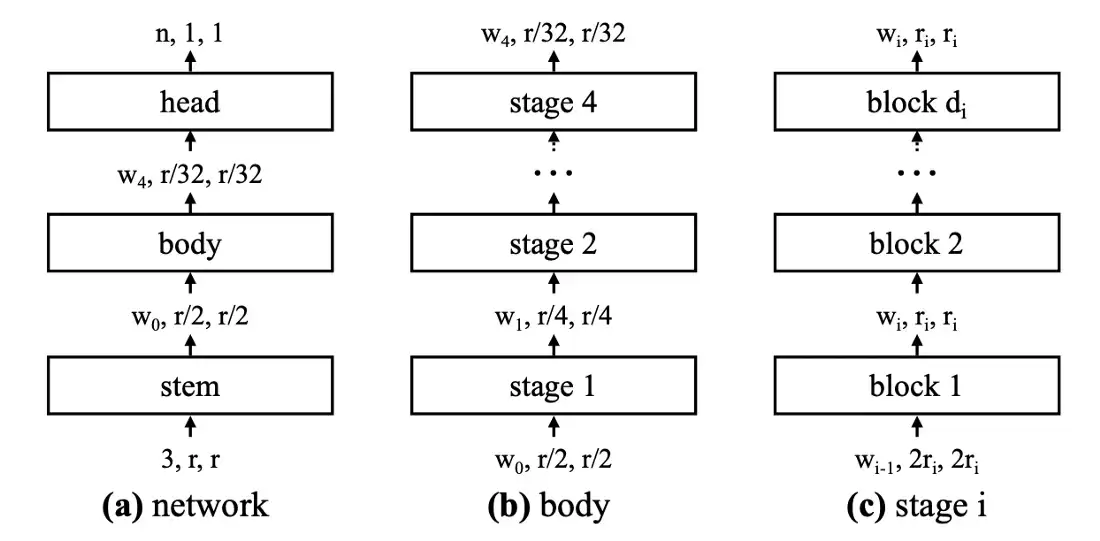
\includegraphics[width=0.95\textwidth]{img/regnetbody2.jpg}
        \small{Fonte: Imagem retirada do artigo \citep{designspace}.}
    \end{figure}

    Um ponto de atenção citado pelos autores é a decisão de manter todos os blocos iguais e com a
    mesma estrutura de uma ResNet \citep{DBLP:journals/corr/HeZRS15}. A imagem~\ref{fig:regnet2} a seguir exemplifica:

    \begin{figure}
        \caption{Exemplo de um bloco \textbf{X} baseado em uma rede residual.}
        \centering
        \label{fig:regnet2}
        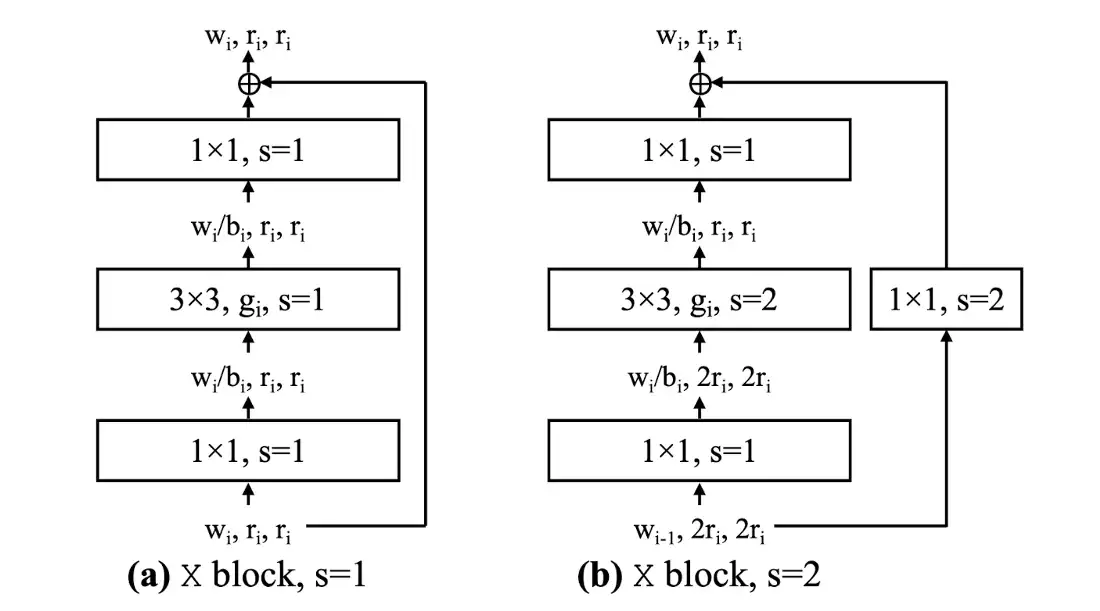
\includegraphics[width=0.95\textwidth]{img/regnetbody.jpg}
        \small{Imagem retirada do artigo \citep{designspace}.}
    \end{figure}

    \begin{table}[!h]
    \centering
        \caption{Tabela de restrições dos modelos até chegar no modelo RegNet \citep{designspace}. O índice $i$ é o
    estágio, fixado em 4. O $b_{i}$ representa
    razão do gargalo, $g_{i}$ representa o total de canais da convolução , $d_{i}$ representa o
        total de blocos e o $w_{i}$ represnta o tamanho do bloco.}
    \label{tab:any}
    \begin{tabular}{l|l|c|l|l}
    & restriction & dim. & combinations & total \\
    \hline AnyNet \(_{\mathrm{A}}\) & none & 16 & \((16 \cdot 128 \cdot 3 \cdot 6)^{4}\) & \(\sim 1.8 \cdot 10^{18}\) \\
    AnyNet \(_{\mathrm{B}}\) & \(+b_{i+1}=b_{i}\) & 13 & \((16 \cdot 128 \cdot 6)^{4} \cdot 3\) & \(\sim 6.8 \cdot 10^{16}\) \\
    AnyNet \(_{\mathrm{C}}\) & \(+g_{i+1}=g_{i}\) & 10 & \((16 \cdot 128)^{4} \cdot 3 \cdot 6\) & \(\sim 3.2 \cdot 10^{14}\) \\
    AnyNet \(_{\mathrm{D}}\) & \(+w_{i+1} \geq w_{i}\) & 10 & \((16 \cdot 128)^{4} \cdot 3 \cdot 6 /(4 !)\) & \(\sim 1.3 \cdot 10^{13}\) \\
    AnyNet & \(+d_{i+1} \geq d_{i}\) & 10 & \((16 \cdot 128)^{4} \cdot 3 \cdot 6 /(4 !)^{2}\) & \(\sim 5.5 \cdot 10^{11}\) \\
    RegNet & quantized linear & 6 & \(\sim 64^{4} \cdot 6 \cdot 3\) & \(\sim 3.0 \cdot 10^{8}\)
    \end{tabular}
    \end{table}

    A tabela~\ref{tab:any} explica um pouco como o modelo RegNet é montado. Como citado
    anteriormente, é possíveis infinitas combinações de arquitetura de redes neurais dependendo dos
    parâmetros a serem testados. A primeira arquitetura de rede neural, \textbf{AnyNetA}, não possui nenhuma restrição,
    totalizando aproximadamente $1.8 \cdot 10^{18}$ combinações possíveis. No último modelo, após
    adicionar todas as restrições e avaliar todas as \textbf{AnyNets} o modelo enfim chega no Regnet
    utilizando uma metodologia conhecida como \textit{quantized linear parameterization}, para que
    todo os blocos do mesmo estágio tenham o mesmo tamanho.

    A desempenho dos modelos amostrados do NDS é calculada através de um procedimento que se resume
    em treinar o modelo no conjunto de dados ImageNet \citep{5206848} por 10 épocas~\ref{sec:batch}
    e calcular o erro de inferência nesse mesmo conjunto de dados. É amostrado em torno de 100
    modelos para cada NDS com seu conjunto de parâmetros e restrições.

    \begin{figure}
        \centering
        \caption{A imagem da esquerda mostra os \textit{Design Spaces} A, B, e C, sendo o C mais
        restritivo entre eles. A imagem da direita mostra a distribuição de erro de cada desses
        espaços, sendo o C aquele que possui melhor desempenho entre eles.}
        \label{fig:space}
        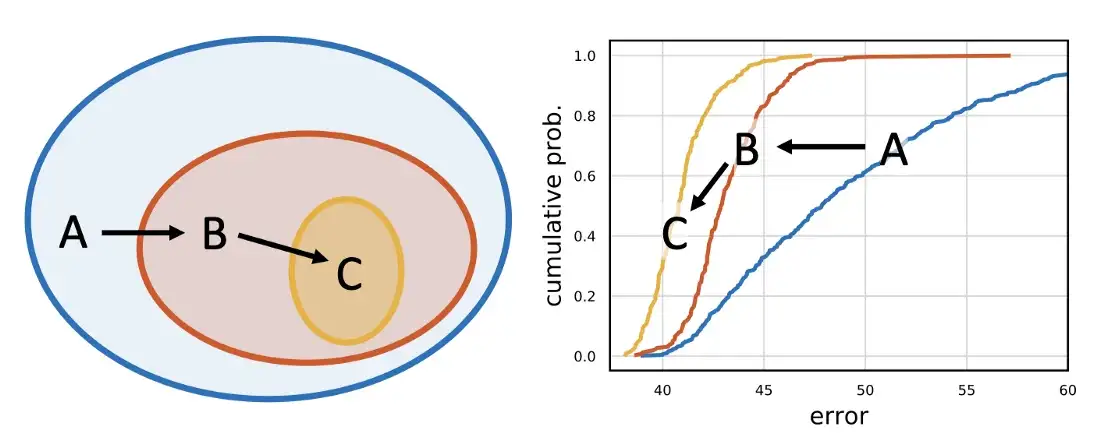
\includegraphics[width=0.95\textwidth]{img/design_space.jpg}
        \small{Fonte: Imagem retirada do artigo \citep{designspace}.}
    \end{figure}

    Ao final, os autores chegam a conclusão que os modelos amostrados do espaço\textbf{RegNet} possuem desempenho
    melhor do que os modelos amostrados do \textbf{AnyNet} para qualquer valor dos parâmetros
    escolhidos. Além disso, os autores apresentam o modelo \textbf{RegNetY} que é uma variação do
    \textbf{RegNetX} contendo uma técnica conhecida como \textit{squeeze-and-excitation}
    \citep{squeeze} para
    que cada bloco seja capaz de adaptar os pesos para capturar as partes mais importantes da imagem
    com um adicional de custo computacional baixo.

    \section{Conceitos}

    \subsection{Camadas}\label{sec:layer}

    As camadas são onde se encontra os neurônios ou unidades de processamento. Um rede neural
    normalmente possui múltiplas camadas, ou pelo menos duas, camada de entrada e saída. Quanto mais
    camada a rede neural possuí mais profunda ela é, ou seja, mais neurônios são utilizados. No
    entanto, é necessário tomar cuidadado, pois quanto mais neurônios mais calculaos e dados são
    necessários para utilizar o modelo, demandando mais poder computacional.

    \subsection{Pesos ou Parâmetros}\label{sec:weight}

    As redes neurais é composta por várias unidades de processamento, cujo o funcionamento é o mais
    simples possível. As unidades das redes neurais, conhecido também como neurônios, são
    interligados entre si, e cada um dessas unidades possui um peso, também conhecido como
    parâmetro. As unidades fazem operações matematicas com os dados locais, sendo estes dados
    as entradas processada por outra unidade de processamento ou uma tabela de dados se esta unidade estiver na
    primeira camada do modelo, também conhecida como camada de entrada, do inglês \textit{input
    layer}.

    A fígura~\ref{fig:redeneuralmlp} representa uma MLP contendo três camadas. Uma camada de entrada,
    uma camada intermediária e uma camada de saída. Cada uma desses camadas possui um número N de
    neurônios. Cada neurônio, ou unidade de processamento, possui conexões com outras unidades,
    sendo essa conexão seria o \textbf{peso} ou \textbf{parâmetro}. O peso então é múltiplicado pela saída de
    um neurônio que entra em um próximo neurônio. Dentro do neurônio, todas as entradas são somadas e em seguida
    passa o resultado da soma em uma função de ativação, como por exemplo uma sigmoid
    \citep{GoodBengCour16}, para transformar ou limitar os valores. Todos os neurônios de uma camada
    possuí ligações com todos os neurônios da próxima camada.

    \begin{figure}
        \centering
        \caption{Uma rede neural MLP, com 3 camadas. Uma de entrada com 3 neurônios,uma camada
        intermediária com 4 neurônios e uma de saída com dois neurônios.}
        \label{fig:redeneuralmlp}
        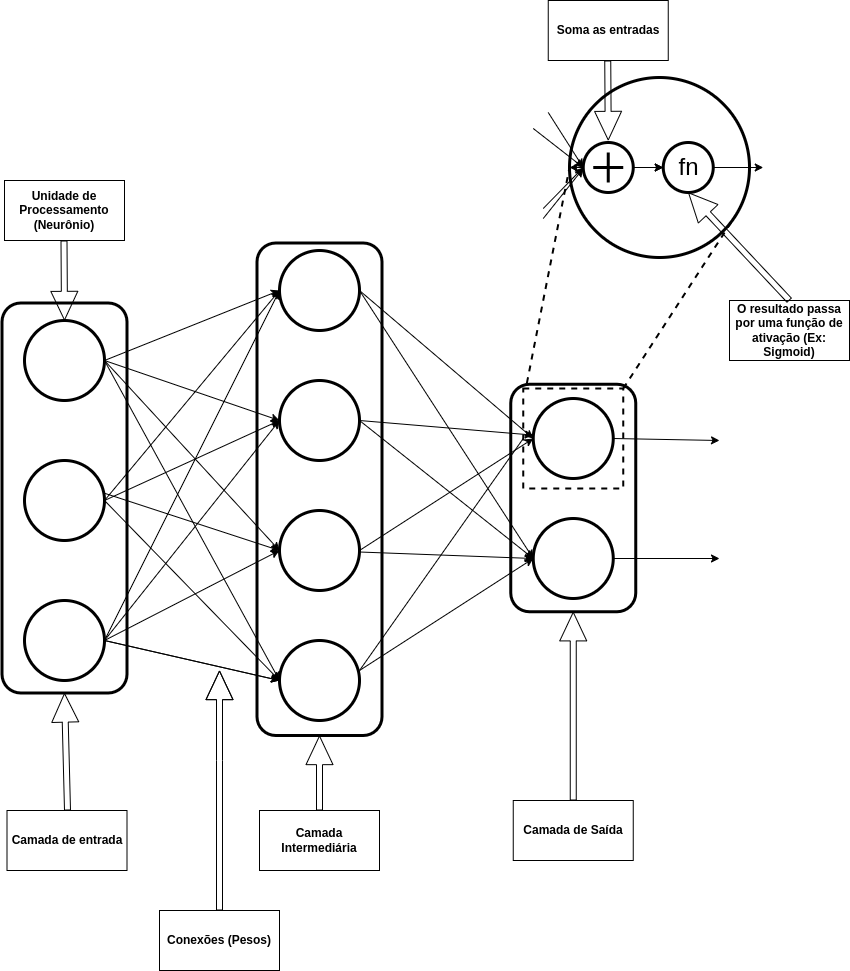
\includegraphics[width=0.6\textwidth]{./img/rede_neural_4.png}
        \small{Fonte: Imagem elaborada pelo autor.}
    \end{figure}

    \subsection{Taxa de aprendizado}\label{sec:learningrate}

    A taxa de aprendizado é o valor de atualização dos pesos. Toda vez que uma rede neural erra sua
    previsão ou resposta, é necessário que estes pesos se ajustem, de forma a diminuir o valor do
    erro. A taxa de aprendizado é o tanto que esta atualização vai mudar o peso. Quanto mais alta a
    atualização maior o valor atualizado, e quanto menor menor será essa mudança. É necessário
    balancear este valor para que as atualizações sejam em tamanho corretos para que o modelo
    consiga chegar em um mínimo local quanto a métrica de erro \citep{GoodBengCour16}.

    \subsection{Treino, Teste e Inferência}

    O processo pasa se obter e usar um modelo de aprendizado de máquina é divide em três fases: treino,
    teste e inferência. O treino é a fase onde ajustamos os parâmetros do modelo para que ele
    complete uma tarefa da melhor forma possível, que neste projeto seria diagnosticar o glaucoma. O
    teste é a fase onde avaliamos a desempenho do modelo utilizando as métricas previamente
    estabelecidas. E a fase de inferência é quando um modelo já treinado e avaliado será utilizado
    pelo público alvo. Normalmente, os modelos na fase de inferência são
    colocados na nuvem\footnote{Infraestrutura de computação necessários para rodar uma aplicação
    que seja acessado através da internet. Os recursos virtuais refletem uma infraestrutura física
    local, com servidores, memórias, clusters e armazenamentos. Tudo isso voltado
    para uma escabilidade e fácil uso.} ou em alguma infraestrutura computacional local para que possam ser acessados
    e utilizados e por consequência traga valor para o negócio \citep{GoodBengCour16}.

    Cada uma dessas fases possuem seu conjunto de dados. É necessário ressaltar que se deve ter
    cuidado em dividir o conjunto de dados do treinamento e do teste para que não haja vazamento de
    dados entre os dois conjuntos e o modelo atinja uma desempenho que não representa a realidade.
    O conjunto de dados da inferência vem da utilização do modelo, ou seja, todos aqueles dados
    que não estavam presente dentro do conjunto de treino e teste e é totalmente novo para o modelo.
    Após um certo tempo, normalmente incluem os dados de inferência dentro do conjunto de dados de
    treino e teste e o modelo é retreinado e reavaliado.


    \subsection{Batch e Época}\label{sec:batch}

    O treinamento se divide em épocas. Cada época é uma passagem por todos os dados dentro do
    conjunto de dados treinamento e teste para o modelo, para que este então possa ajustar os seus pesos
    (parâmetros). No entanto, não é possível passar todos os dados para o modelo de uma única vez
    dêvido ao custo computacional e ao tamanho limitado da memória.
    Logo, os dados é dividos em \textit{minibatches} que nada mais são
    que um subgrupo de um grupo de dados. O tamanho deste subgrupo é ajustado de acordo com a tarefa
    e recursos computacionais disponíveis. No entanto, o ideal é que ele seja menor que o grupo todo
    e maior do que 1. Neste último caso, o modelo precisará fazer muitas atualizações e também usara
    recurso computacional excessivamente, além de que, a generalização poderá ser afetada para pior
    já que 1 amostra dificilmente irá representar ou aproximar mínimamente a distribuição de dados
    do conjunto todo \citep{GoodBengCour16}.

    \subsection{Função de perda}\label{sec:loss}

    A função de perda mede o quão longe da resposta correta o modelo está. Também conhecida como
    \textbf{função de custo}, esta função irá indicar a qualidade do modelo e quais são os valores
    de atualização necessárias para os parâmetros utilizando apenas um número real. O que esta função faz é
    comparar o que é conhecido como \textit{ground truth}\footnote{\textit{Ground truth} é uma
    informação que sabemos que é real utilizando métricas ou através da observação.} com a saída do
    modelo. Neste projeto o \textit{ground truth} é a classe dos dados, indicando presença ou
    ausência do glaucoma.

    \subsection{Otimizadores}\label{sec:optimizer}

    Os otimizadores são algoritmos ou funções responsáveis por atualizar os parâmetros dos modelos.
    O otimizador acha o melhor valor para esses parâmetros com o objetico de diminuir o erro do modelo
    em uma devida tarefa. Dado isso, o otimizador recebe os parâmetros do modelo, a taxa de
    aprendizado e o erro através da função de custo, e com todos estes recursos e dados, o otimizador escolhe a
    melhor atualização para os parâmetros. Contudo, é essencial escolher o melhor
    otimizador para cada uma das tarefas ou modelos que serão utilizados. Desta forma,o aprendizado
    do modelo possa ser efetivo e o modelo consiga desempenhar com qualidade.

    \subsection{Hiperparâmetros}\label{sec:hyper}

    Os hiperpâmetros dos modelos são configurações de cada um destes modelos ligado ao processo de
    aprendizado. Por exemplo, citado anteriormente\ref{sec:learningrate}, a taxa de aprendizado é
    um hiperparâmetro a ser escolhido e indica a magnitude de atualização dos parâmetros. Outro
    hiperparâmetro é o tamanho do \textit{minibatch}
   ~\ref{sec:batch} e também qual otimizador~\ref{sec:optimizer} será utilizado \citep{GoodBengCour16}. Normalmente, para
    encontrar os melhores hiperpâmetros para o modelo é necessário repetir o processo de treino e
    teste múltiplas vezes, tornando este processo extremamente caro.

    %Desta forma, para otimizar a
    %busca de hiperparâmetros ideal para os modelos e arquiteturas deste projeto, foi utilizado uma
    %ferramente conhecida como \textit{Optuna}\ref{sec:optuna}. A ferramente utiliza formas inteligentes de encontrar
    %o melhor hiperpâmetros, diminuindo a necessidade de testar todas as combinações e reduzie o
    %custo computacional.


    \subsection{Sobrajuste}\label{sec:overfitting}

    O sobreajuste, do inglês \textit{overfitting}, é um cenário onde o modelo se ajusta de forma
    quase que perfeita para um conjunto de dados X e por conseqência, acaba tendo uma perda de
    desempenho no conjunto de dados Y que possui uma distribuição diferente de X. É ideal que o
    modelo consiga generalizar bem para todos os conjuntos de dados disponíveis, no entanto, é
    praticamente impossível já que qualquer comportamente diferente nos dados pode causar
    distribuições totalmente diferentes entre eles. Logo, se conjunto de dados X e Y possuem
    distribuições próximas, mas não iguais, é possível utilizar de um para conseguir inferir o
    outro. POrtanto, se o modelo sobreajusta para X e tenta inferir Y, este modelo irá ter um erro
    grande quanto a sua inferência, já que apesar das distribuições serem próximas, a distribuição de
    X é diferente de Y \citep{GoodBengCour16}.

    Com isto, para se evitar o sobreajuste do modelo, este projeto aplicou uma técnica conhecida como
    \textit{Early Stopping}~\ref{sec:trainval}. A técnica tem como intuito parar o processo de
    treinamento quando o modelo começa a aumentar sua desempenho no conjunto de dados de treino (X) e
    sofre uma piora significativa no conjunto de dados de teste (Y) utilizado para avaliação.
    A fígura~\ref{fig:overfitting} a seguir mostra visualmente como acontece o sobreajuste.

    \begin{figure}
        \centering
        \caption{Uma imagem representando o problema de sobreajuste e subajuste.}
        \label{fig:overfitting}
        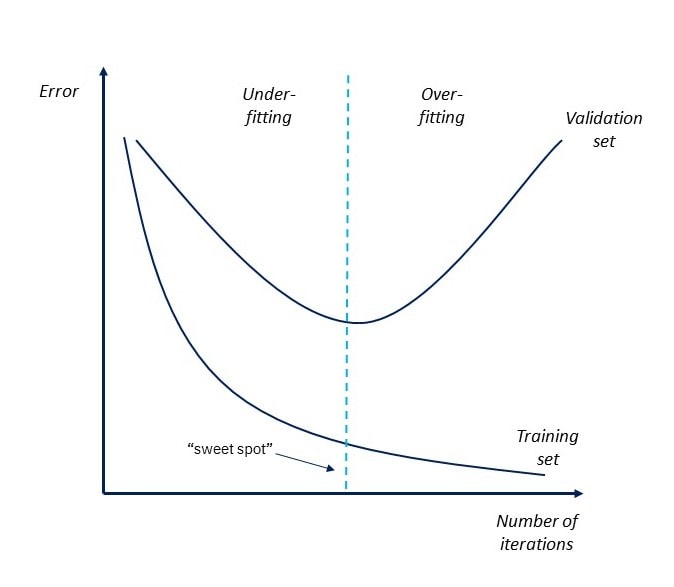
\includegraphics[width=0.6\textwidth]{./img/classic_overfitting.jpg}
        \small{Fonte: \href{https://www.ibm.com/cloud/learn/overfitting}{IBM}}
    \end{figure}


    \subsection{Convolução}\label{sec:conv}

    As convoluções funcionam como filtros que enxergam pequenos quadrados e vão “escorregando” por
    toda a imagem captando os traços mais marcantes. Explicando melhor, com uma imagem
    32$\times$32$\times$3 e um
    filtro que cobre uma área de 5$\times$5 da imagem com movimento de 2 saltos (chamado de stride), o
    filtro passará pela imagem inteira, por cada um dos canais, formando no final um \textit{feature
    map} ou \textit{activation map} de 28$\times$28$\times$1. A image~\ref{fig:convexp} mostra como uma convolução
    funciona.

    \begin{figure}
        \centering
        \caption{Exemplo de uma convolução com filtro 5$\times$5. Cada quadrado com este tamanho
        produz um número com utilizndo operações matemáticas. Em seguida, o quadrado é deslocado
        para o lado ou para baixo e um novo filtro é formado.}
        \label{fig:convexp}
        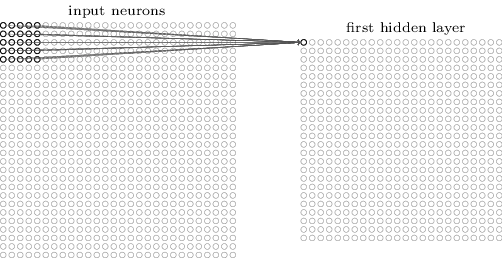
\includegraphics[width=0.6\textwidth]{./img/convoex.jpg}
        \small{}
    \end{figure}


    A profundidade da saída de uma convolução é igual a quantidade de filtros aplicados (Total de canais).
    Quanto mais profundas são as camadas das convoluções, mais detalhados são os traços
    identificados com o \textit{activation map}. No entanto, quanto maior o número de canais, maior
    será o número de operações e consequentemente uma demanda maior de hardware.


    \section{Arquiteturas}
    \label{sec:arqui}

    Neste projeto foram testadas 4 arquiteturas de modelos. Não confudir com arquitetura de
    redes neurais. Cada uma das arquiteturas visuais apresentadas a
    seguir será testada com diferente combinações de hiperparâmetros. O intuito de testar diferentes
    arquiteturas é que cada uma delas pode se sair melhor à depender da tarefa a ser realizada e os
    dados disponíveis. Dado isso, iremos testar as seguintes arquiteturas mostradas na
    fígura~\ref{fig:arqui}.


    \begin{figure}[h]
    \caption{Arquitura de modelos. O \textit{backbone} pode ser um dos modelos citados
    anteriormente (RegNet, ResNet, Inception e etc), e o
    \textit{classifier} é uma rede neural de múltiplas camadas (MLP), assim como o modelo \textit{MLP}
    que recebe os dados tabelados e também o que faz operação de concatenar (\textit{concat})
    juntando todas as saídas e passar para o classificador.}
    \label{fig:arqui}
    \begin{subfigure}[h]{0.48\textwidth}
        \centering
        \caption{Arquitetura utilizando uma imagem de olho (Single Input)}
        \label{fig:arqui1}
        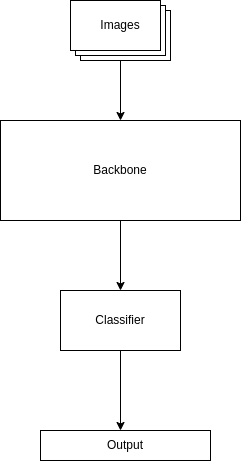
\includegraphics[width=0.78\textwidth]{./img/arqui1.png}
        \vspace{4ex}
    \end{subfigure}%%
    \begin{subfigure}[h]{0.48\textwidth}
        \centering
        \caption{Arquitura utilizando uma imagem do olho e os dados tabulados (Single Input Tabular)}
        \label{fig:arqui2}
        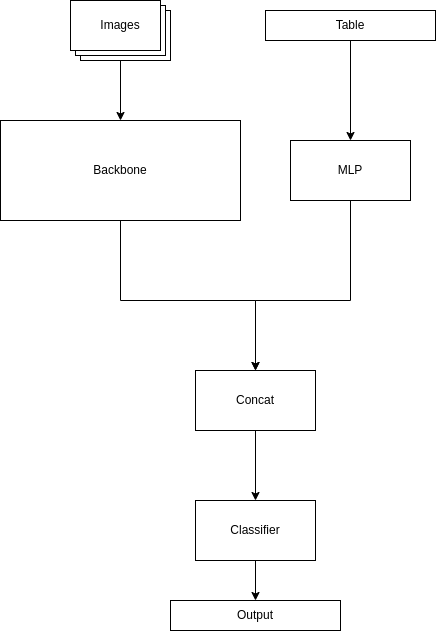
\includegraphics[width=0.78\textwidth]{./img/arqui4.png}
        \vspace{4ex}
    \end{subfigure}
    \begin{subfigure}[h]{0.48\textwidth}
        \centering
        \caption{Arquitetura utilizando duas imagens do mesmo olho (Dual Input)}
        \label{fig:arqui3}
        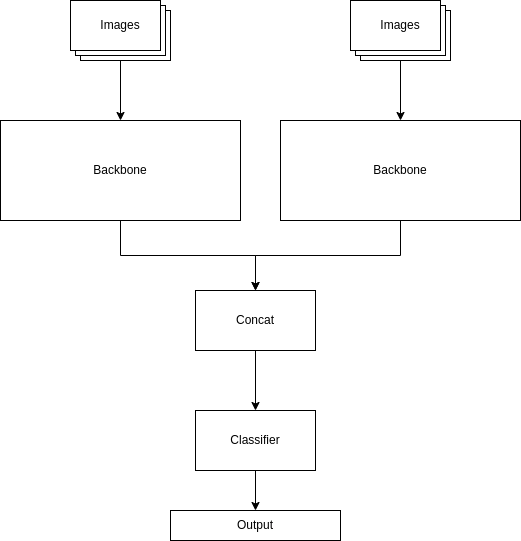
\includegraphics[width=0.78\textwidth]{./img/arqui2.png}
        \vspace{4ex}
    \end{subfigure}
    \hfill
    \begin{subfigure}[h]{0.48\textwidth}
        \centering
        \caption{Arquitetura utilizando duas imagens do mesmo olho e os dados tabulados (Dual Input
        Tabular)}
        \label{fig:arqui4}
        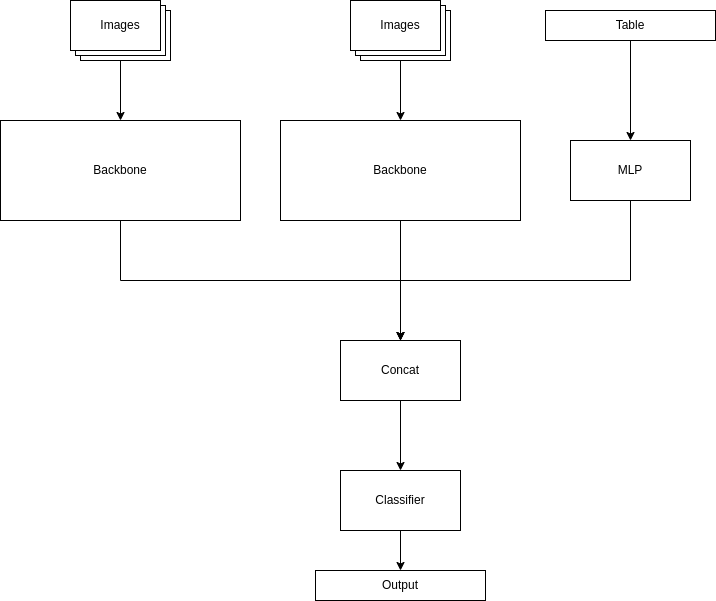
\includegraphics[width=0.78\textwidth]{./img/arqui3.png}
        \vspace{4ex}
    \end{subfigure}
    \small{Fonte: Imagem elaborada pelo autor.}
    \end{figure}

    Todos as arquiteturas de modelos citados na fígura~\ref{fig:arqui}, representados por um retângulo e com exceção
    do \textit{backbone}, é um modelo de múltiplas camadas (MLP). Os modelos \textit{backbone},
    com tradução literária de \textit{espinha dorsal}, são os modelos principais e os utilizados
    para extrair os padrões mais importantes dos dados. No nosso caso, estes dados serão um conjunto
    de imagens de fundo de olho.

    A primeira arquitetura (SI)~\ref{fig:arqui1} utilizará somente uma imagem do fundo do olho. Entre
    asarquiteturas citadas na fígura~\ref{fig:arqui} esta é a arquitetura mais simples e que utiliza a menor quantiade de
    recurso computacional. Além disso, temos a arquitetura que utiliza uma imagem do fundo de olho e
    os dados tabelados do OCT~\ref{fig:arqui2}. Esta segunda arquitetura junta os dados de imagens e os dados
    clínicos para trazer mais informações e consequentemente ajudar na classificação/diagnóstico da
    presença/ausência do glaucoma (SIT).

    A terceira arquitura (DI)~\ref{fig:arqui3} utiliza duas imagens do fundo de olho. Para que isso fosse possível, foi
    feita uma limpeza dos dados e uma avaliação manual de cada uma das fotos para cada paciente da
    base de dados. Escolhendo uma foto mais próxima e outra mais distante.
    A limpeza de dados é descrita e explicada na seção~\ref{sec:limpeza}. A quarta e última
    arquitetura é a que utiliza duas imagens do fundo do olho e os dados clinícos. Esta é a
    arquitetura que utiliza mais recurso computacional, dado que o modelo de imagem é
    duplicado (\textit{backbone}), utilizando o dobro de memória e adicionamos uma rede
    MLP para processar os dados clinícos (DIT).

    Um \textbf{ponto de atenção}, a arquitetura de modelo utilizando somente uma imagem, seleciona
    aleatoriamente uma das duas imagens disponíveis para processar. Desta forma, este modelo aprende
    tanto a trabalhar com imagens mais próximas e mais distantes. Para o modelo que utiliza duas
    imagens, cada imagem passa por um \textit{backbone} diferente. Logo, o mesmo padrão de imagem passa em cada
    um dos modelos, ou seja, imagens mais próximas são processadas por um modelo de imagem e imagens
    mais longes são processadas pelo segundo modelo de imagem.  Desta forma, cada \textit{backbone}
    fica responsável por aprender um padrão de cada uma das imagens. Isto é feito tanto no processo
    de treinamento do modelo quanto no processo de testagem e inferência, quando o modelo já está
    treinado e é utilizado.

    \section{Métricas de Avaliação}
    \label{sec:metrics}

    Para modelagem de diagnóstico na área médica, as métricas certas devem utilizadas para que
    possamos avaliar a qualidade do modelo com robustez. Neste projeto, as métricas utilizadas são:

    \begin{itemize}
        \item Sensibilididade (SN): É a capacidade do modelo de ser acertivo ao fazer diagnósticos positivo
            quanto a presença do glaucoma no paciente.
        \item Especificidade (SP): É a capacidade do modelo em detectar todos os casos verdadeiros de
            glaucoma.
        \item Caracterítica de Operação do Receptor (ROC): Esta curva ajuda os profissionais e
            desenvolvedores do modelo a escolher um limiar de corte entre sensibilididade e especificidade
            que esteja de acordo com o problema de negócio. Esta métrica é a mais importante e
            utilizada em diagnósticos, pois como citado anteriormente, é possível termos uma
            flexibilidade de acordo com a regra de negócio, dado mais importância para sensibilidade
            ou para especificidade \citep{rocc}.
        \item Aréa sob a curva ROC (AUC): Permite verificar o quão bom o clasisficar binário desempenha no
            problema. O cálculo é feito utilizando a área sob a curva ROC. Quanto maior este valor
            mais flexível o modelo consegue ser quanto a especificidade e sensibilididade.
            Esta métrica varia de 0 á 1, sendo o melhor modelo aquele que tem valor igual
            a 1.
    \end{itemize}

    \begin{figure}
    \centering
        \caption{AUC e curva ROC.}
    \label{fig:rocauc}
    \begin{subfigure}[b]{0.5\textwidth}
        \centering
        \caption{Curva ROC}
        \label{fig:curvaroc}
        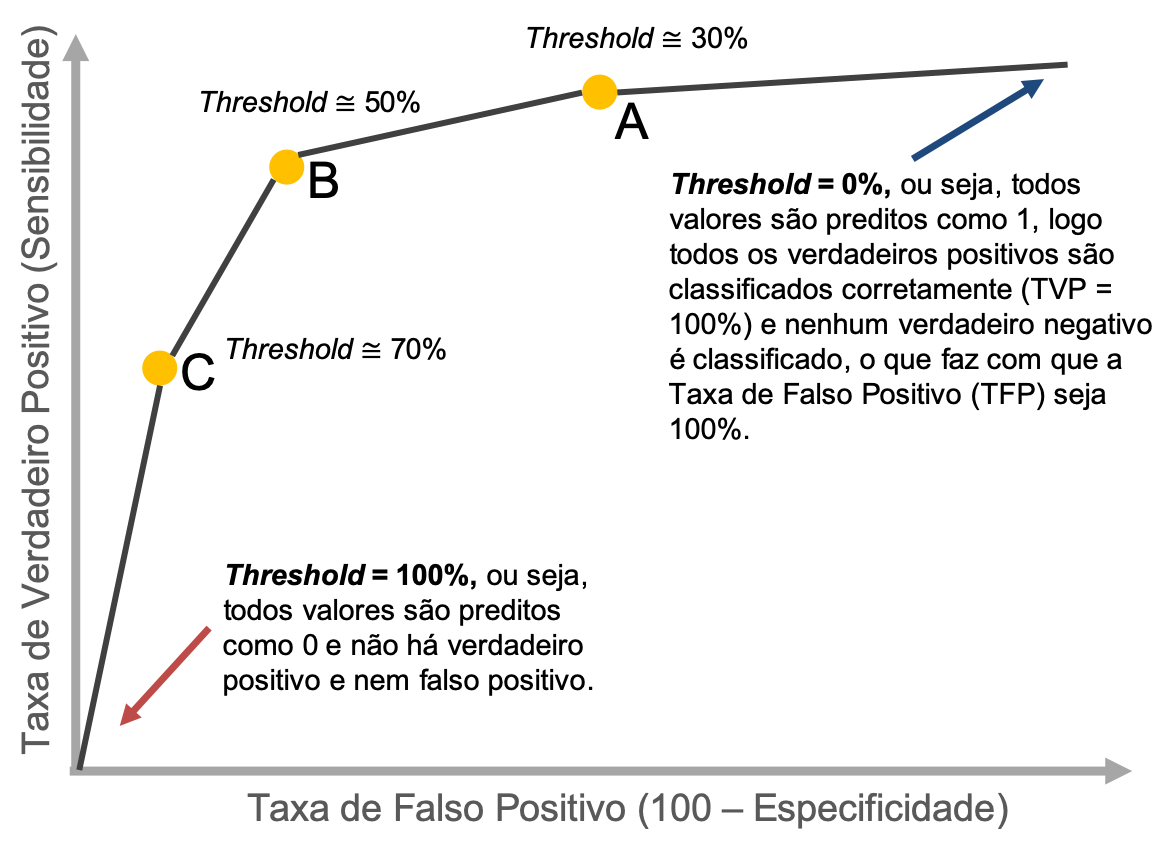
\includegraphics[width=0.98\textwidth]{./img/roc_curvas_threshold.png}
    \end{subfigure}%%
    \begin{subfigure}[b]{0.5\textwidth}
        \centering
        \caption{Area sobre a curva (AUC)}
        \label{fig:auc}
        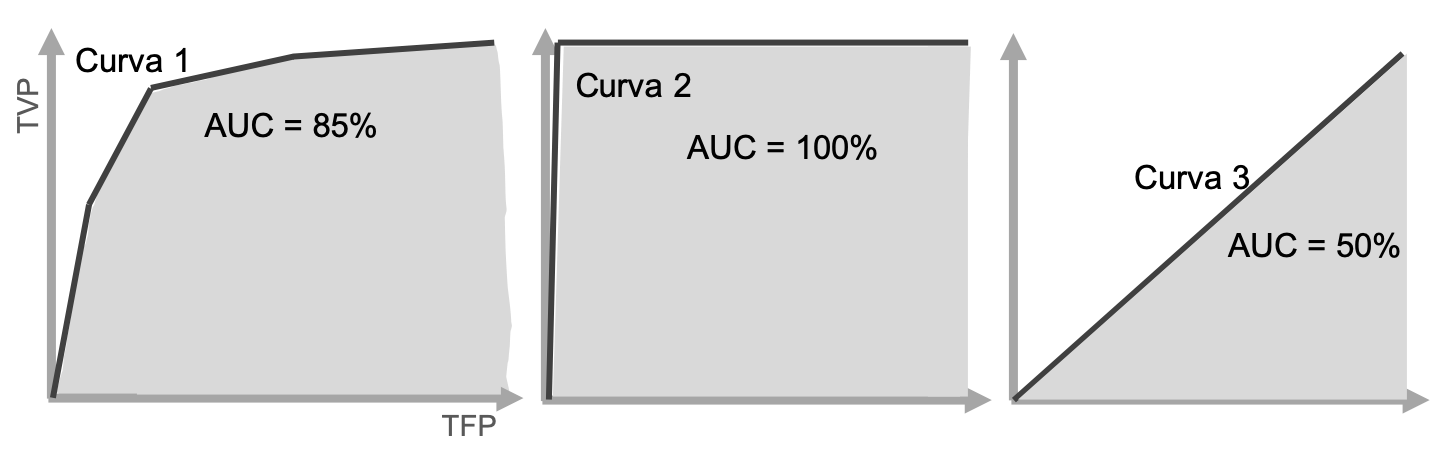
\includegraphics[width=0.98\textwidth]{./img/auc_todas_curvas.png}
    \end{subfigure}
        \small{Fonte:
        \href{https://cienciaenegocios.com/curva-roc-e-auc-em-machine-learning}{Ciencias e Negocios,
        2020}}
    \end{figure}


    Para selecionar o melhor modelo entre todos os experimentados, iremos utilizar a AUC como
    métrica principal, já que esta métrica consegue sumarizar, utilizando somente um número, o quão bom
    a curva ROC se encontra para cada um dos modelos. A fígura~\ref{fig:rocauc} explica, de forma
    ilustrativa, como a curva ROC e a AUC funcionam.  Em aplicações médicas, é mais válido trazer o maior
    número de verdadeiro positivos sem aumentar significativamente a taxa dos falsos positivos.
    Normalmente é mais prejudicial deixar de diagnosticar uma doença do que dar um diagnóstico
    positivo falso. Neste caso, o interesse maior é na sensibilidade. No entanto, se abaixarmos o
    threshold demais iremos ter bastante falso positivos, ou seja, muito casos para serem análisados
    pelos especialista, gerando um custo humano e de tempo~\ref{fig:curvaroc}. As duas métricas, sensibilidade e
    especificidade, interegem entre si. Quando se aumenta uma, movimentando threshold, é possível
    que se perca desempenho na outra. Contudo, o valor da métrica AUC carrega consigo a informação de
    variação desse ganho e dessa perda, ou seja, quanto melhor o AUC mais fácil movimentar o
    threshold ganhando de um lado e abdicando menos do outro. O modelo perfeito, com 100\% de AUC,
    na imagem da direta~\ref{fig:auc}, mostra que se movimentarmos o threshold não perderíamos nada, e
    seria possível capturar todos os casos verdadeiro sem nenhum caso de falso positivo.
    No entanto, é impossível construir um modelo perfeito, e normalmente os modelos ficam entre 50\% e 100\%.


    \section{RandAugment}
    \label{sec:aug}

    \textit{Data Augmentation} \citep{data_aug} é uma técnica de aumento do número de dados de forma sintética. Neste
    caso, operações são aplicadas na imagem de forma que novas imagens sejam criadas a
    partir das originais e por fim aumentando heterogeneidade do dados para modelagem. Com os dados
    mais heterogeneo é possível atingir desempenhos melhores para o modelo sem aumentar de forma
    exponencial o custo computacional (mais poder computacional) que por fim será refletido em custo
    real.

    \par Para realizar o \textit{Data Augmentation} utilizamos neste projeto o
    \textit{RandAugment} \citep{randaug}. De acordo com os autores, o \textit{RandAugment} traz
    benefícios como: diminuir drásticamente o uso computacional pois não se utiliza políticas para
    escolher as operações a serem aplicadas nas imagens, mas sim uma probabilide X de acontecer para
    cada um delas. Desta forma, é possível manter a diversidade das imagens e ter um custo baixo
    para isso. As transformações possíveis são: transformação identidade,
    auto-contraste, equalizador, rotação, solarização, cor tremida, mudança de contraste, mudança de
    brilho, posterização, mudança de formato, translações e cortes.

    \par Uma decisão feita para a utilização do \textit{RandAgument} é que ele só foi aplicado nos
    modelos que tiverram a melhor desempenho entre todos os outros. Evitando assim, que infinita combinações
    sejam testadas e ao mesmo tempo fosse possível avaliar o benefício da tecníca.

    \section{Treinamento e Avaliação dos Modelos}
    \label{sec:trainval}

    Os modelos foram treinados e avaliados utilizando uma técnica conhecida como validação cruzada, do
    inglês \textit{cross-validation}. A validação cruzada tem como objetivo avaliar a capacidade de
    generalização de um modelo a partir de um conjunto de dados. Busca-se então estimar o quão
    preciso é este modelo na pratica, ou seja, o desempenho para um novo conjunto de dados. Dado
    isso, iremos utilizar o método K-Fold \citep{cross-val}. Os autores do artigo \citep{overview}
    citam que dentre o processo de treinamento e validação, a validação cruzada é uma das mais
    utilizadas.

    O método K-Fold consiste em separa os dados em K partes, sendo que K-1 partes serão utilizadas
    para o treino do modelo e a parte restante será utilizada para validação do modelo. Em uma
    próxima iteração um novo grupo é selecionado para teste e os outros K-1 para treino, até que
    todos os grupos passem pela fase de teste. Com isto, é possível que o modelo seja avaliado com
    mais robustez e com variabilidade controlada.

    \begin{figure}[h]
        \centering
        \caption{Imagem contendo ilustrando a validação cruzada. Cada parte assume o papel de teste
        uma vez e treino K-1 vezes.}
        \label{fig:cross}
        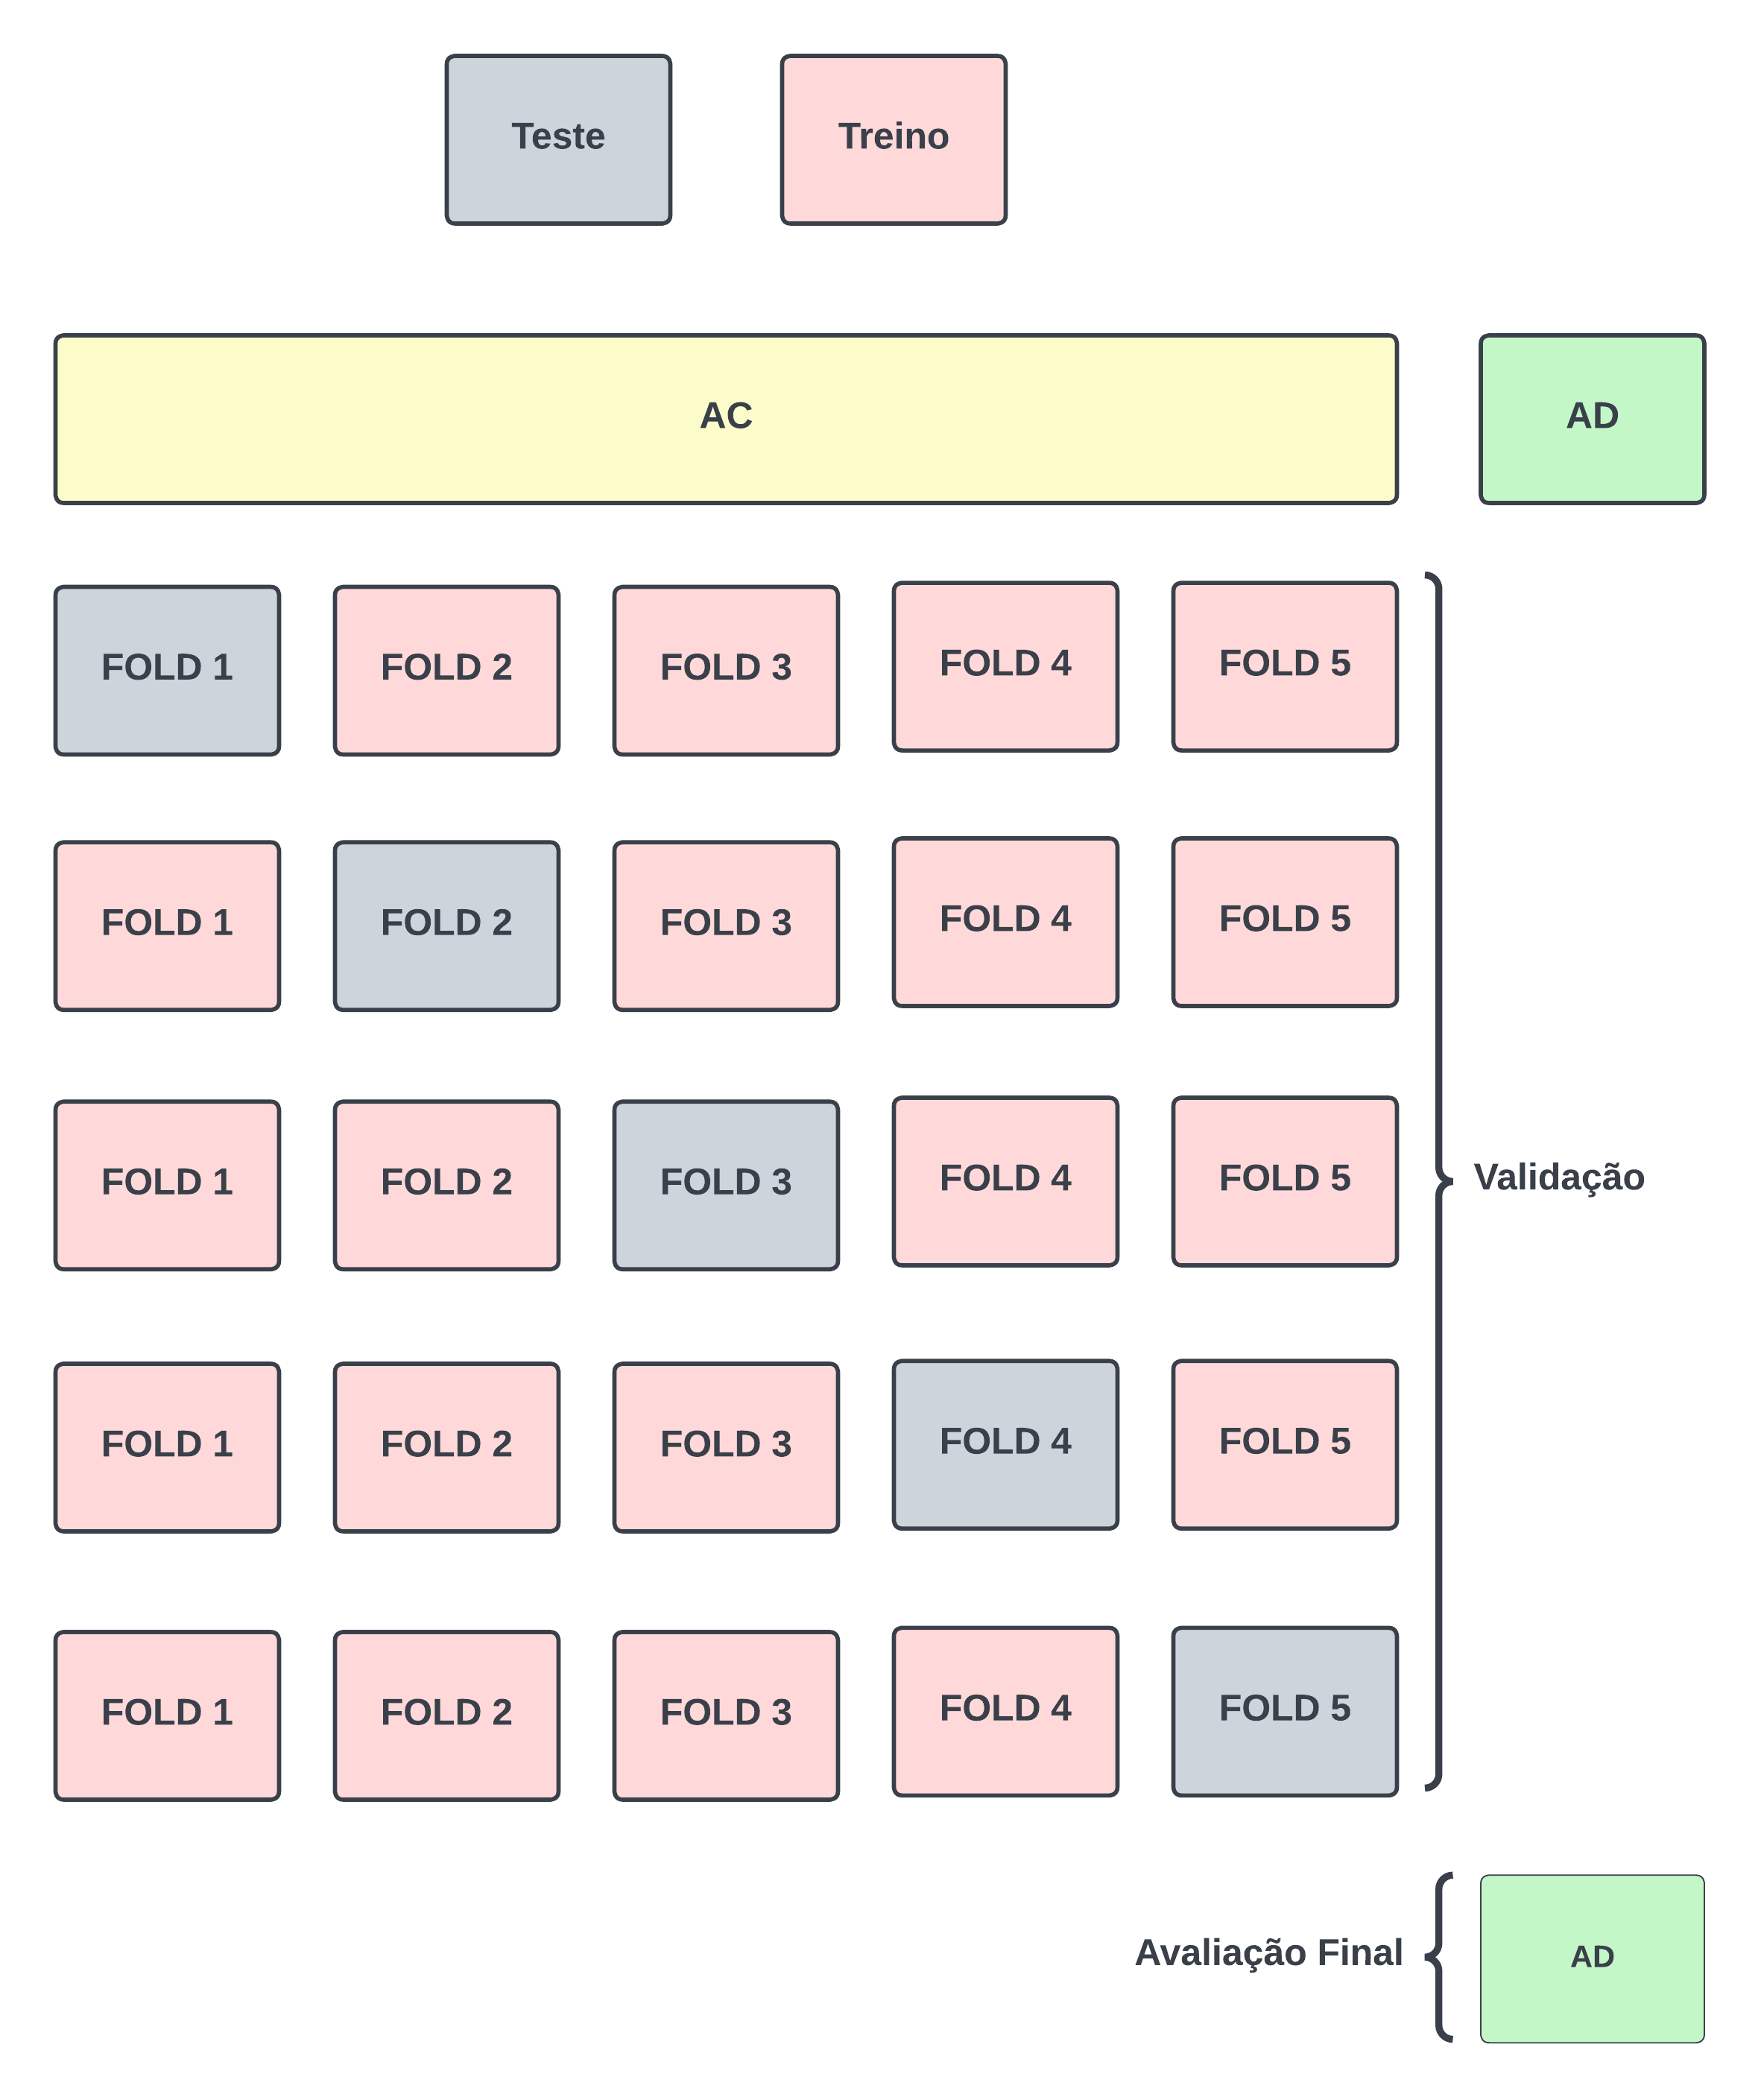
\includegraphics[width=0.98\textwidth]{./img/cross.png}
        \small{Fonte: Elaborado pelo autor.}
    \end{figure}

    A imagem~\ref{fig:cross} mostra como os dados são divididos. Existem dois conjunto de dados que
    são AC (Amostras Conhecidas) e o AD (Amostras Desconhecidas). Dado isso, utilizando o conjunto
    AC aplicando a metodologia de validação cruzada, validando assim os melhores modelos. Em
    seguida, utilizados o conjunto AD para mensurar o desempenho do modelo. Este conjunto AD não
    entra nas iterações da validação cruzada, portando é possível avaliar a capacidade de
    generalização do modelo em dados que simulam os dados na etapada de inferência.

    Além disso, para que não houvesse \textit{overfitting} \citep{GoodBengCour16} do modelo utilizamos o
    \textit{Early Stopping} para finalizar o treinamento quando o modelo não melhora sua desempenho
    durante um número E de épocas. Adicionado à isso, economizamos também no custo computacional. E
    por fim, foram salvos so melhores modelos para cada experimento de acordo com a métrica
    escolhida, \textbf{AUC}.

    \section{Explicabilidade: SHAP}
    \label{sec:shap}

    O SHAP (Shapley Additive Explanations) é uma das ferramentas mais utilizadas quando o assunto é
    explicabilidade. O objetivo por trás do SHAP é trazer um entendimento quanto a decisão de
    modelos complexos, modelos antes conhecidos como caixa preta devido sua falta de
    interpretabilidade. Logo, modelos estatísticos como XGBoost, LightGBM e modelos profundos como
    redes neurais convolucionais (CNN) agora são possíveis de serem entendidos ou interpretados
    \citep{NIPS2017_7062}.

    A interpretação dos modelos trouxe uma forma inovadora de aplicar modelos de aprendizado de
    máquina, principalmente na área de saúde. O modelo interpretável traz informações extra para que
    o profissional seja capaz de tomar melhores decisões quanto ao problema que enfrenta.

    Modelos foram propostos para diagnosticar e verificar a progressão da
    evolução da doença de Alzheimer \citep{El-Sappagh2021}. Os autores aplicam o modelo SHAP para pegar as características
    que são mais críticas para o modelo. O modelo SHAP foi capaz de dar explicações sobre quais
    características mais impactam a progressão da doença. Além disso, o modelo também forneceu
    explicações individuais para cada um dos pacientes. E em seguida foi utilizado um sistema
    baseado em lógica fuzzy \citep{fuzzy} e linguagem natural para poder criar um formulário que os médicos e os
    pacientes pudessem consumir a explicação do modelo.

    Utilizando modelos mais simples, como Árvores de Decisão \citep{quinlan:induction},
    Regressão Logística \citep{cox1958regression} e kNN \citep{kNN} e
    modelos mais complexos, como SVM \citep{svm}, XGBoost \citep{DBLP:journals/corr/ChenG16}, e
    RF \citep{breiman2001random}, os autores criaram
    um sistema de prognóstico da doença de hepatite \citep{PengJunfeng2021AEAI}. Os autores
    utilizaram o modelo SHAP para verificar as variáveis
    mais importantes para os modelos, fornecem explicação para cada um dos pacientes e também
    geraram gráficos de dependência entre as váriaveis de entrada e a rótulo dos dados (presença ou
    ausência de hepatite).

    Utilizando modelos como XGBoost \citep{DBLP:journals/corr/ChenG16} para selecionar qual cirurgia refratória
    deve ser aplicada em um paciente \citep{10.1167/tvst.9.2.8}. A escolha certa de uma cirurgia aumenta a satisfação de um
    paciente ao final do processo. Antes da escolha da cirurgia, o paciente consulta um expert da
    área e em seguida 80 características da tomografia da cornea são extraídas, 40 características
    demográficas são coletadas e mais 22 características de exames oftamológicos, como por exemplo diâmetro da
    pupila. Ao final, os autores fazem uma validação cruzada de 10 grupos e atinge uma acurácia
    média de 72\% quanto a cirurgia a ser aplicada. Os autores também apresentam as características
    globais mais importantes e para cada um dos 3 exames aplicados: LASEK, LASIK, SMILE e
    contraindicação.

    O shap utiliza o que chamamos de \textit{Shapley Values} ou valores de \textit{Shapley}. Os
    valores de \textit{Shapley} é uma média ponderada da contribuição marginal de cada um das
    características \citep{shapley1988shapley}. Isto é caracterizado pelo impacto que cada um destas
    características tem no valor preditivo do modelo \citep{strumbel}.

    \begin{figure}[h]
        \centering
        \caption{Gráfico sumarizado para o dataset Boston Housing ordenado pelas características
        mais importantes do modelo.}
        \label{fig:boston}
        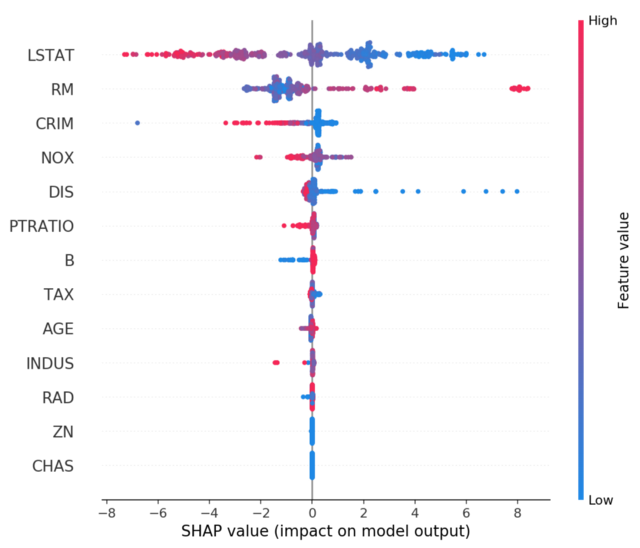
\includegraphics[width=0.98\textwidth]{./img/shap_boston.png}
        \small{Fonte: \href{https://github.com/slundberg/shap}{SHAP Github}}
    \end{figure}

    Na figura~\ref{fig:boston} representa um gráfico SHAP para previsão dos preços de moradias em
    Boston-MA. Se o ponto é azul a variável apresentação um valor baixo, se o ponto é vermelho ela
    apresenta um valor alto. Se o ponto está do lado direito quer dizer que aquele valor da variável
    contribui para a resposta seja positiva ou maior, se do lado esquerdo, negativa ou menor. Por exemplo, a variável
    mais importante é a \textbf{LSTAT}. É a proporção de adultos sem ensino superior e a proporção
    de trabalhadores braçal ou árduo masculinos em uma certa área. Significa que quanto maior essa
    proporção menor será um preço das casas na vizinhança. Enquanto a variável \textbf{RM} é a
    quantidade de quartos nas casas. Quanto mais quartos na casa maior será o valor atribuído para aquela
    residência.


    \begin{figure}
        \centering
        \caption{Explicação de uma imagem utilizando SHAP. Os pontos vermelhos e azul mostram onde o
        modelo julgou como parte importante para a imagem. Seguindo a mesma lógica
        do~\ref{fig:boston}, pontos vermelhos aumenta a probabilidade na saída do modelo, enquanto
        pontos azuis diminuem.}
        \label{imgshap}
        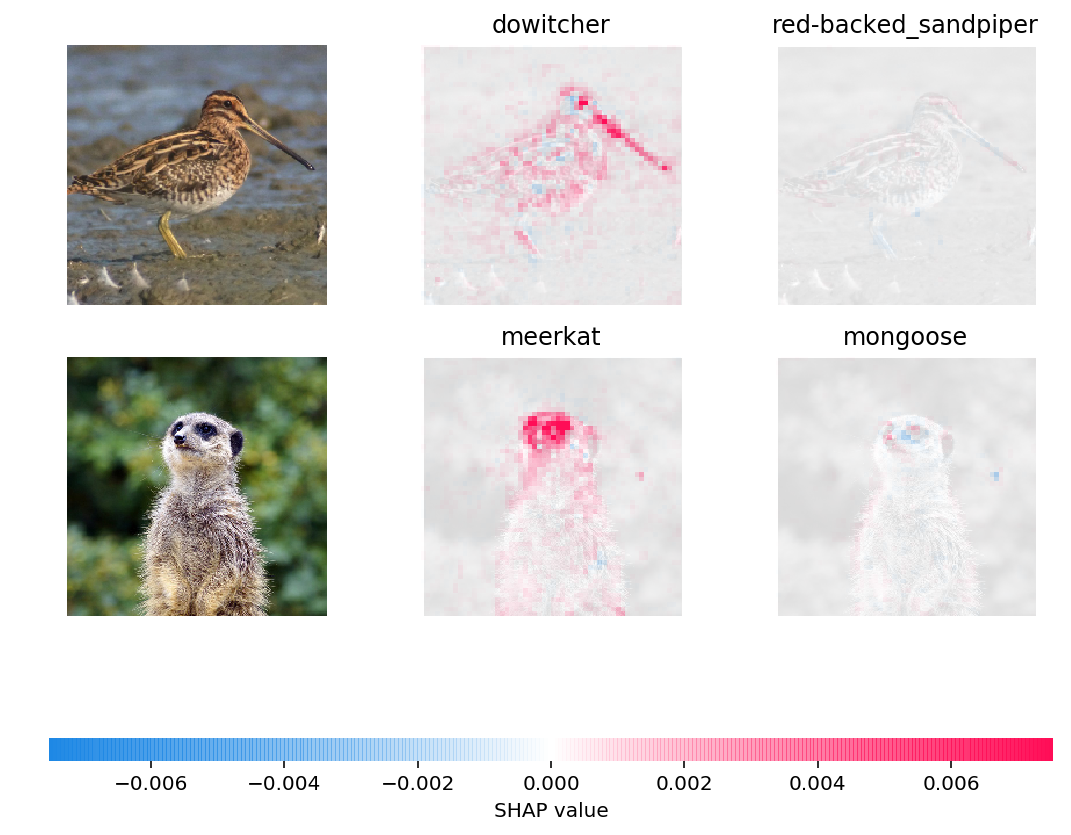
\includegraphics[width=0.98\textwidth]{./img/gradient_imagenet_plot.png}
        \small{Fonte: \href{https://github.com/slundberg/shap}{SHAP Github}}
    \end{figure}

    No entanto, para imagens, o SHAP funciona um pouco diferente. Na fígura~\ref{imgshap} a
    explicabilidade do modelo fornce quais são as áreas das imagens mais importantes para
    identificação de um animal. Por exemplo, para o passaro podemos observar que existem vários
    pontos vermelhos fortes na mesma área do bico, indicando dessa forma que essa parte foi uma das
    mais importantes para a identificação do passáro.


    \chapter{Sumário e Preprocessamento dos dados}
    \label{preprocessing}

    \section{Sumário dos dados}


    O dado recebido possui múltiplas imagens de fundo de olho para cada paciente. As imagens estão
    divididas para cada um dos olhos que foram feitos os exames. Foram recebidos um total de 492
    pacientes e 887 olhos. Além disso, também está presente nos dados uma tabela contendo algumas
    informações do paciente e do exame OCT. Na tabela contém os seguintes dados:
    \begin{itemize}
        \item Dados demográficos: Nome, Idade, Gênero
        \item Presença ou ausência do glacoma
        \item Indicação do olho examinado: esquerdo ou direito. Quando não há indicação, ambos os
            olhos foram examinados
        \item Medições de espessura das fibras retiradas do OCT: região nasal (N), nasal inferior (NI), nasal
            superior (NI), temporal (T), temporal inferior (TI), temporal superior (TS) e a média de todos os
            quadrantes (G).
    \end{itemize}

    Um exemplo na fígura~\ref{fig:fundus2} contendo duas imagens do fundo dos olhos:

    \begin{figure}[ht]
    \centering
    \caption{Duas imagens do fundo do olho com distâncias diferentes}
    \label{fig:fundus2}
    \begin{subfigure}[t]{0.48\textwidth}
        \centering
        \caption{Imagem do fundo do olho distante do disco e copo}
        \label{fig:fundus2a}
        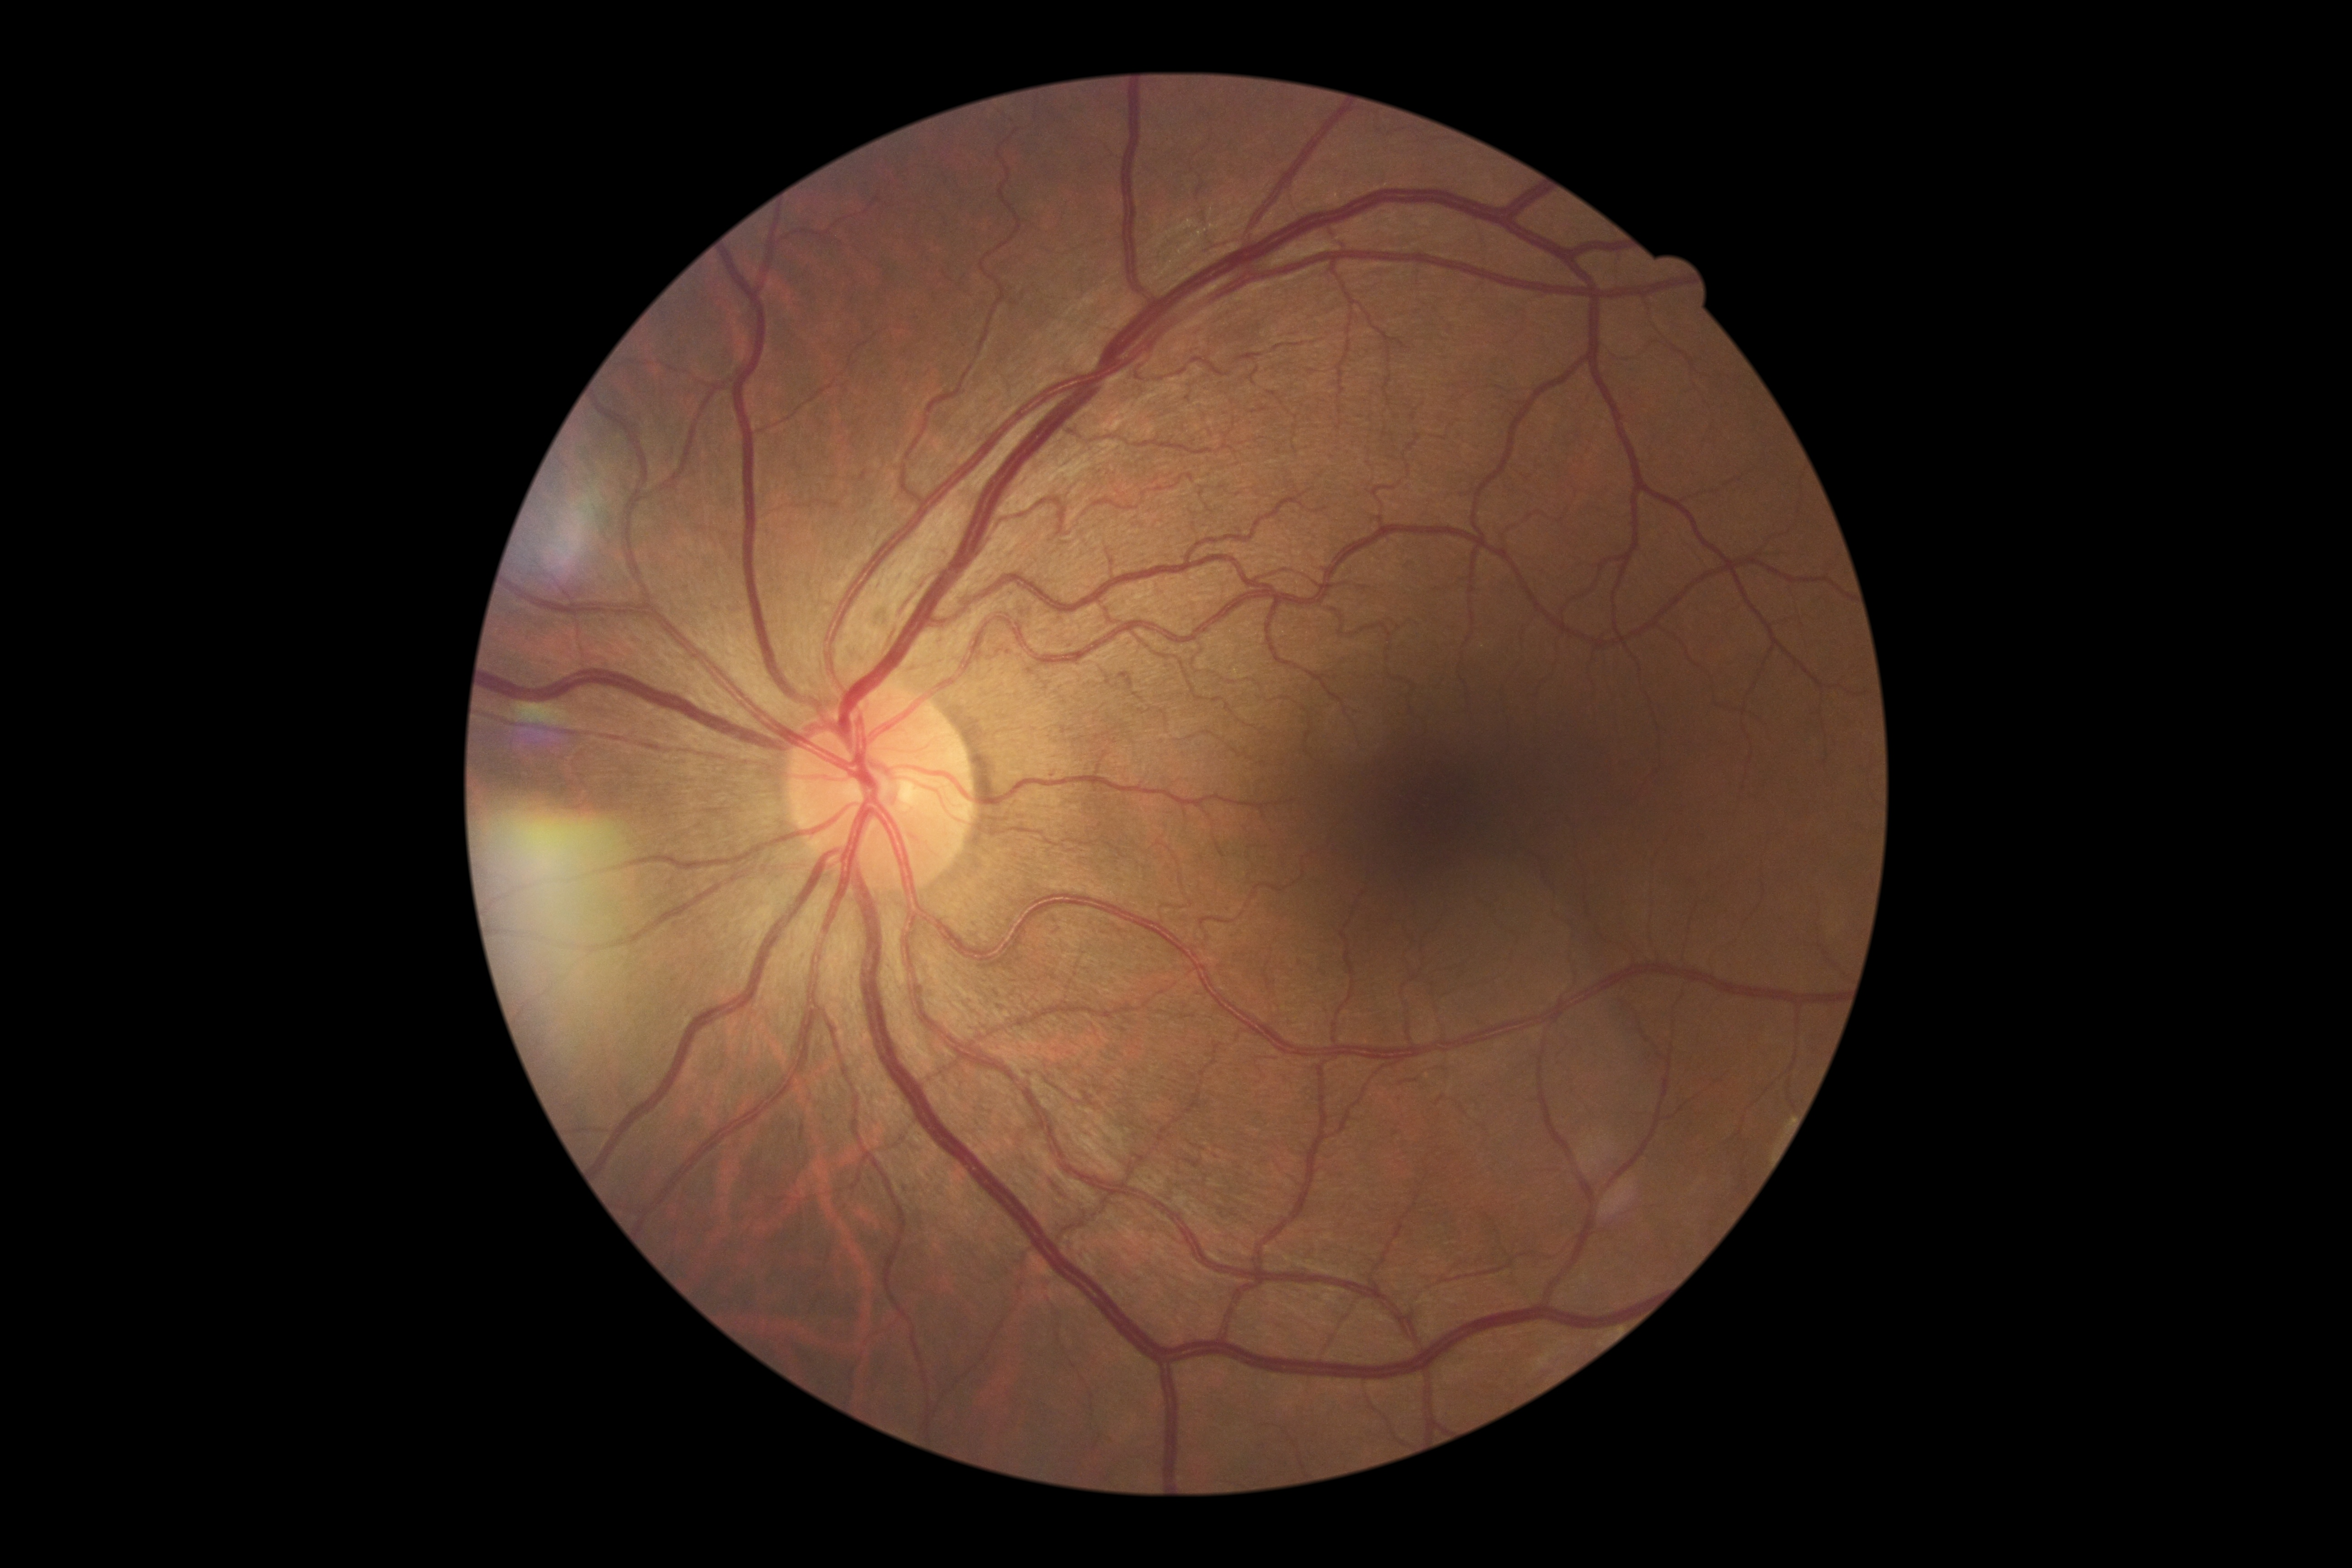
\includegraphics[width=0.9\textwidth]{./img/foto1fundus.jpg}
        \hspace{2ex}
    \end{subfigure}\hfill
    \begin{subfigure}[t]{0.48\textwidth}
        \centering
        \caption{Imagem do fundo do olho próxima do disco e copo}
        \label{fig:fundus2b}
        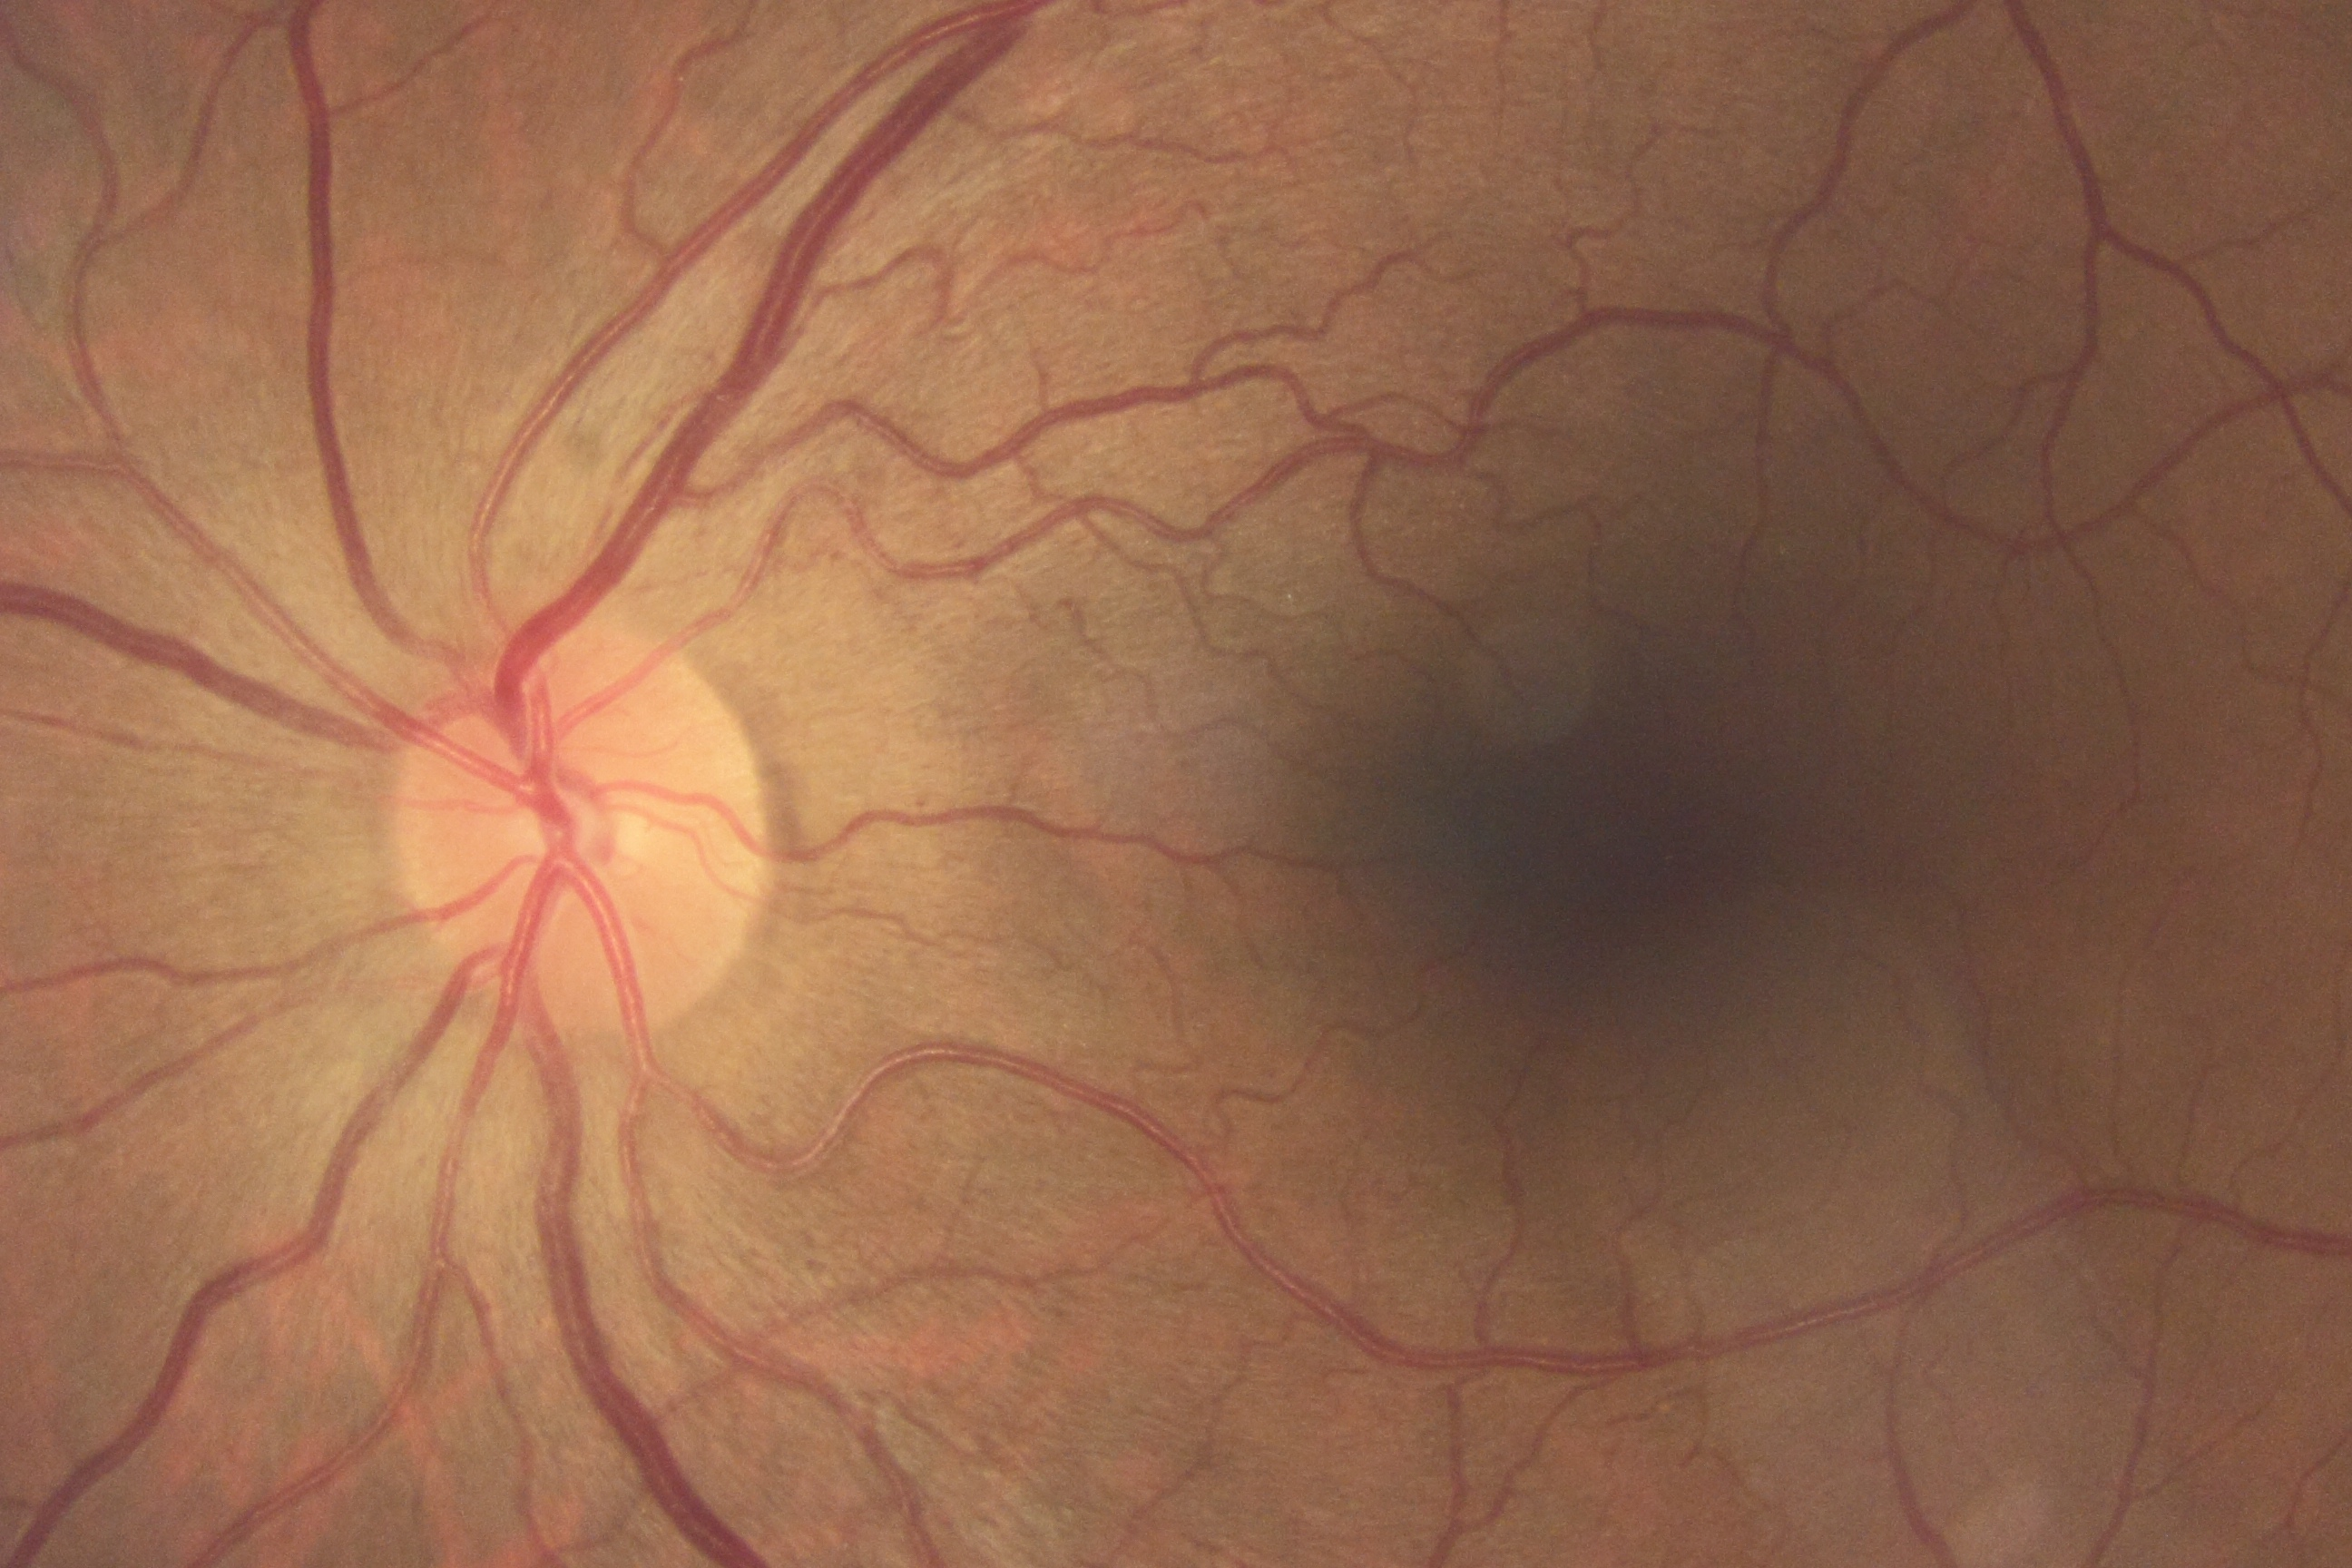
\includegraphics[width=0.9\textwidth]{./img/foto2fundus.jpg}
    \end{subfigure}
    \small{Fonte: Imagem extraída do conjutno de dados.}
    \end{figure}


    A primeira imagem~\ref{fig:fundus2a} é mais distante quando comparada a segunda imagem
   ~\ref{fig:fundus2b}, que possui um zoom mais próximo do
    disco. Cada paciente testado aqui deve possuir pelo menos duas fotos similares à essa.

    Portnato, na próxima seção, será descrito todo o processo de limpeza dos dados realizados como
    requisitos do experimentos executados neste projeto.

    \section{Limpeza}
    \label{sec:limpeza}

    Antes da exploração e modelagem dos dados, o dado precisa ser padronizado para que todo o processo fique mais
    simples, automatizado e consistente. Em seguida, algumas manipulações manuais foram aplicado aos dados:
    \begin{itemize}
        \item Verificação de duas vias: Verificar se o paciente está presente nos dados tabulares
            e se existe uma pasta contendo fotos do fundo dos olhos.
        \item Foi contabilizado o número de fotos para cada um dos pacientes, sendo assim, grande
            parte dos pacientes possuem pelo menos duas fotos para cada olho. Todos que tivessem uma
            foto ou nenhuma foram eliminados.
        \item Foram selecionadas, de forma manual, duas fotos para cada olho de cada paciente. Uma foto
            mais distante e uma segunda foto mais próxima, sem a parte marginal preta.
            As fotos foram renomeadas para indicar qual das duas imagens é a mais próxima ou
            distante, de forma que o modelo recebe em cada uma das entradas o mesmo tipo de foto.
        \item Foram selecionados somente fotos com cores. Fotos preto e branco foram eliminadas.
        \item Alguns pacientes possuem diferentes datas de exames OCT e imagens do fundo do olhos.
            Dado isso, foi considerado as fotos que estão, em data, mais próximo do dado tabular
            contendo o dia que o exame foi realizado.
    \end{itemize}

    No total de 492 pacientes e 987 olhos, após a limpeza dos dados, restaram 476
    pacientes e 858 olhos que serão utilizados na modelagem.

    \section{Exploração}

    Para entender melhor o problema é necessário que os dados sejam explorados e que a sua
    distribuição seja entendida. Nesta seção iremos avaliar os dados quanto as características
    presentes, como por exemplo, a correlação entre as espessuras das fibras e a presença do
    glaucoma, a presença do glaucoma quanto a idade e o gênero do paciente, e por fim, criar um
    entendimento sólido para dar base aos resultados que irão ser apresentados nas próxima seção.

    \begin{figure}[ht]
    \caption{Contagem de casos de glaucoma por gênero e por olhos}
    \label{fig:explorer}
    \begin{subfigure}[b]{0.5\textwidth}
        \centering
        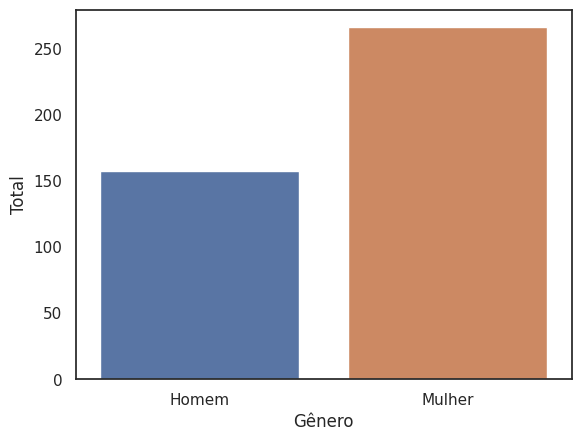
\includegraphics[width=0.75\textwidth]{./img/total_pacientes.png}
        \caption{total de pacientes por gênero}
        \label{figexplorer:a}
        \vspace{4ex}
    \end{subfigure}%%
    \begin{subfigure}[b]{0.5\textwidth}
        \centering
        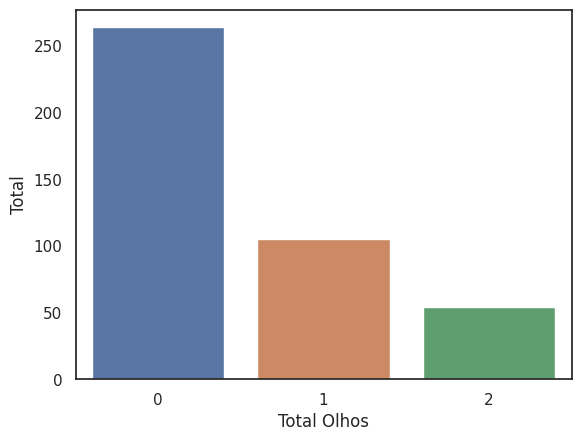
\includegraphics[width=0.75\textwidth]{./img/total_olhos.png}
        \caption{total de pacientes com presença de glaucoma em 0(ausência), 1 ,2}
        \label{figexplorer:b}
        \vspace{4ex}
    \end{subfigure}
    \begin{subfigure}[b]{0.5\textwidth}
        \centering
        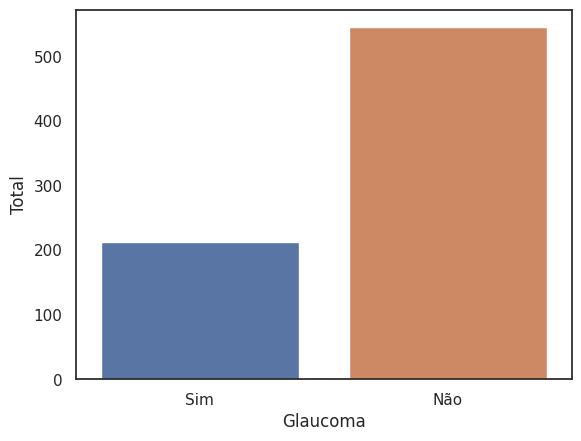
\includegraphics[width=0.75\textwidth]{./img/total_glaucoma.png}
        \caption{Total de olhos com e sem glaucoma}
        \label{figexplorer:c}
    \end{subfigure}%%
    \begin{subfigure}[b]{0.5\textwidth}
        \centering
        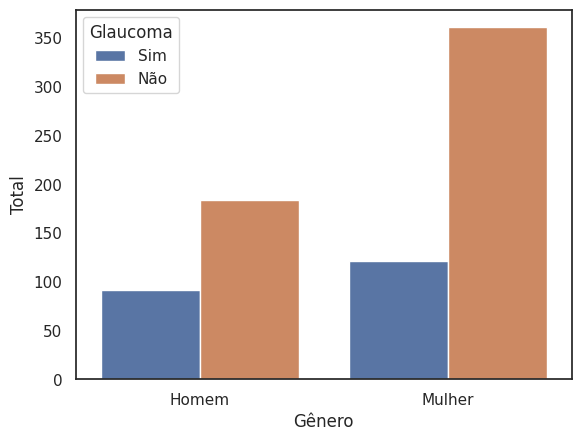
\includegraphics[width=0.75\textwidth]{./img/total_glaucoma_genero.png}
        \caption{Total de olhos com ou sem glaucoma por gênero}
        \label{figexplorer:d}
    \end{subfigure}
        \small{Fonte: Elaborado pelo autor.}
    \end{figure}

    Como podemos obervar nos histogramas da fígura~\ref{fig:explorer} é possível observar que temos mais
    casos de pessoas contendo glaucoma, dentro da base de dados recebida, em somente um dos olhos do que
    nos dois olhos. Além disso, temos a maior presença de pacientes do gênero feminino comparado ao masculino.
    Em proporção, a presençá de glaucoma é maior em homens do que em mulheres. De acordo com Pesquisa Nacional
    Nacional de Saúde \citep{pns}, as mulheres continuam sendo em maior proporção as pessoas que vão
    ao médico e procuram manter-se saudável. Com isto, o dado acima pode ser uma consequência dessa cultura, onde
    temos a maior presença feminina, no entanto, com proporções menores quanto a presença de
    glaucoma. Na seção de resultados, iremos observar se o modelo coloca a variável gênero como uma
    das principais para predição do glaucoma.

    \begin{figure}
        \centering
        \caption{Distribuição do Glaucoma por variável}
        \label{fig:dist_glaucoma}
        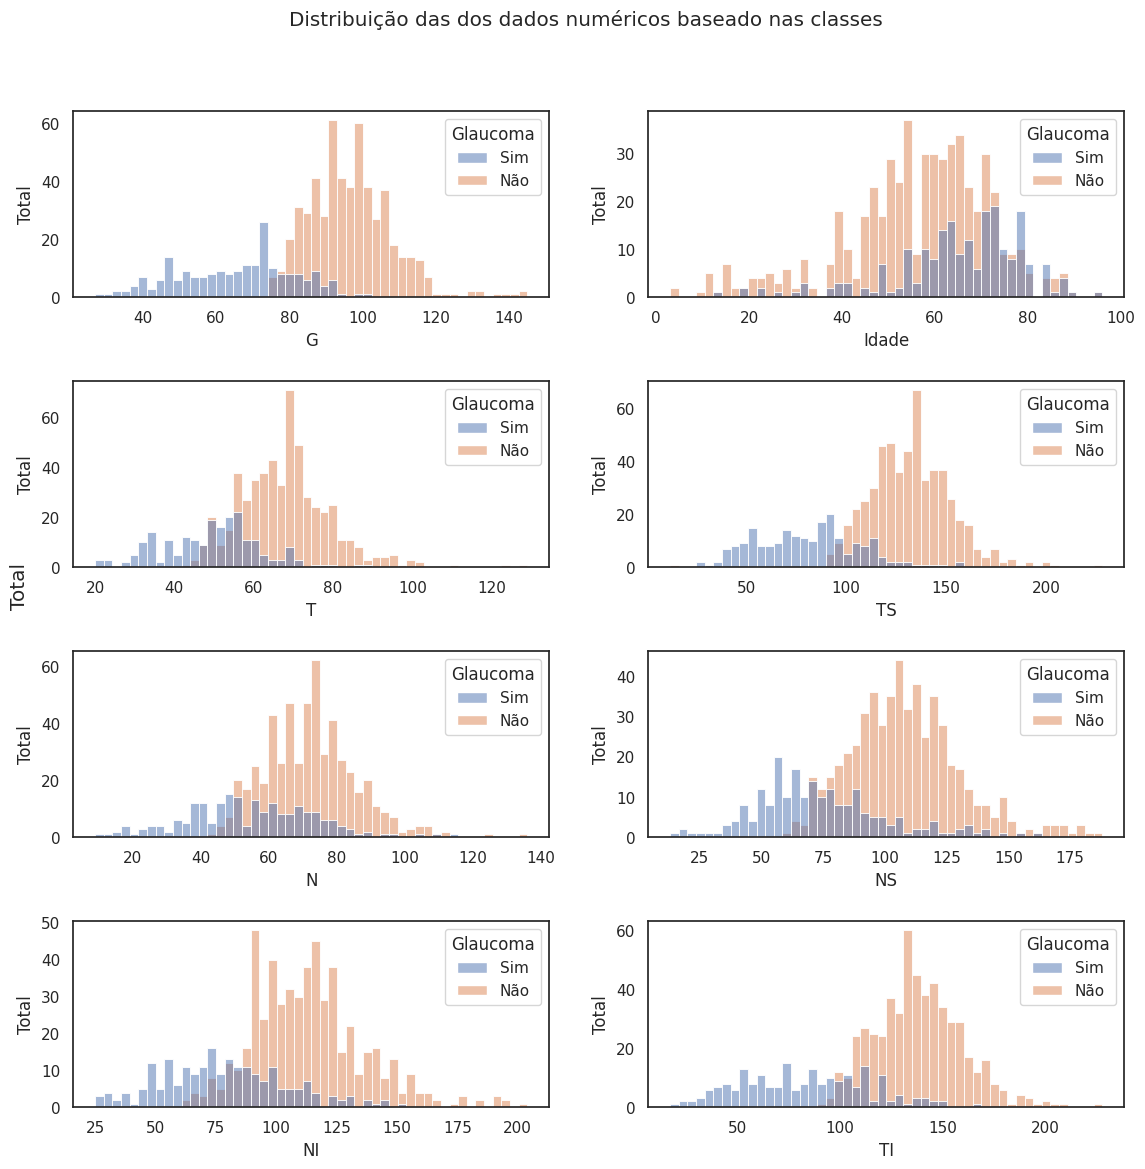
\includegraphics[width=1.0\textwidth]{./img/dist.png}
        \small{Fonte: Elaborado pelo autor.}
    \end{figure}

    Os gráficos da fígura~\ref{fig:dist_glaucoma} mostra a distriuição das variáveis do OCT quanto a
    presença de glaucoma ou não. Existe uma separação visível das distribuições das variáveis G, TS, N e
    TI quanto a presença de glaucoma. Outro ponto importante, é a presença das distribuições contendo caudas
    para esquerda ou para direita. Estes pontos provavelmente serão detectados pelo modelo mais
    fácilmente.

    \begin{figure}
        \centering
        \caption{Boxplot do Glaucoma por variável.}
        \label{fig:boxplot}
        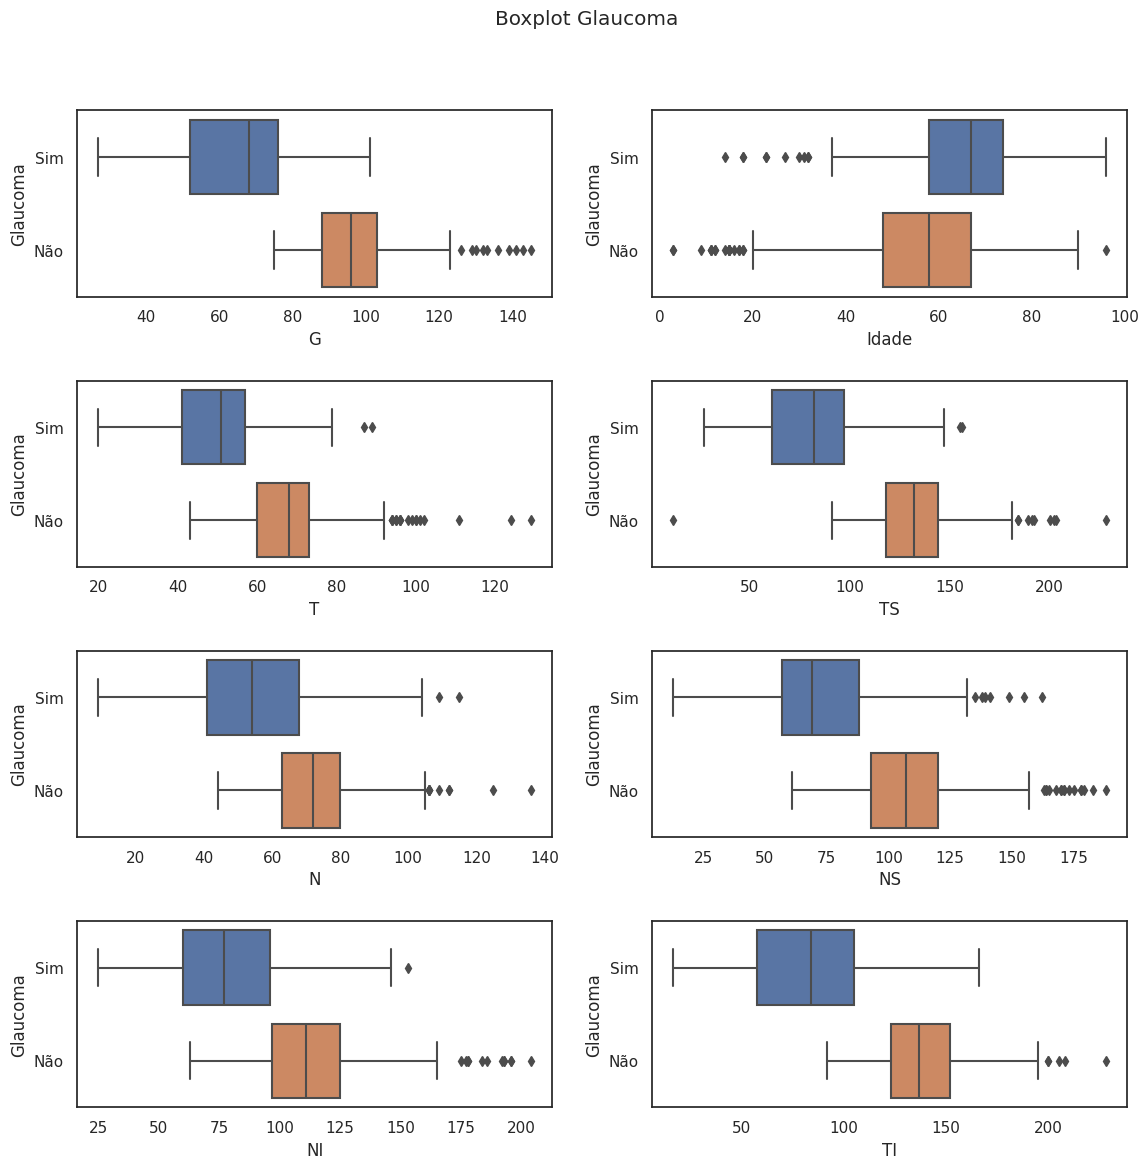
\includegraphics[width=1.0\textwidth]{./img/boxplot.png}
        \small{Fonte: Elaborado pelo autor.}
    \end{figure}

    Existe uma presença de valores atípicos mostrados na fígura~\ref{fig:boxplot}. A idade, como
    mostrado na fígura, pode ser um bom separador, já que existe uma tendência a esquerda (menor
    idade) quando to a ausência do glaucoma.
    As variáveis TI, G e TS são as que mais distanciam os casos quanto a presença ou não do glaucoma.
    Existe uma possibilidade de que essas variáveis sejam umas das mais importantes dos modelos
    para aqueles que usam os dados OCT.


    \begin{figure}
        \centering
        \caption{Correlação absoluta das variáveis}
        \label{fig:corr}
        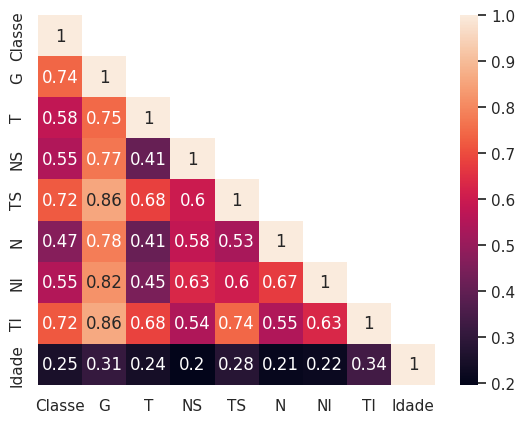
\includegraphics[width=1.0\textwidth]{./img/correlacao.png}
        \small{Fonte: Elaborado pelo autor.}
    \end{figure}

    Existe uma forte correlação entre a variável TS e G~\ref{fig:corr}. Sendo G uma média global, existe a
    possibilidade que a variável TS tenha uma influência forte na média. As variáveis que mais se correlacionam com a
    classe são: TS, TI e G. A seguir, uma sumarização dos dados após a limpeza:

    \begin{table}
    \centering
        \caption{Tabela contendo sumarização dos dados utilizando as estatísticas: máximo, mínimo, média,
        desvio e contagem.}
        \label{tab:estatisticas}
    \csvautobooktabular{./tables/description.csv}
        \small{Fonte: Elaborado pelo autor.}
    \end{table}

    \section{Engenharia de características e Normalização}\label{sec:engineering}

    Quanto a engenharia de características, apenas uma operação matemática foi aplicada. Sabendo que
    uma das características importante para deteção do glaucoma é a razão entre o copo e o disco
    presente no fundo do olho, as características criadas é a razão entre as medições numéricas do
    exame do OCT \citep{pmid31403451}. Desta forma, cada caraterística númerica do OCT irá criar uma característica de
    razão entre pares com as outras. No total, 15 novas características foram criadas para serem
    utilizadas nos modelos. Além de serem características fácilmente criadas, são fáceis de ser
    interpretadas pelos profissionais responsáveis ao análisar os resultados e a explicabilidade do
    modelo.

    A normalização é um processo de redimensionar os valores das características númericas para
    limites entre 0 e 1. A importância da normalização nas redes neurais está diretamente ligado ao
    fato de atualização dos pesos e otimização do modelo.
    Os algoritmos de otimização utilizam a descida gradiente para
    encontrar os melhores valores para diminuir o erro. Dentro da formula de descida gradiente, é
    utilizado os valores das características e da saída do modelo para em seguida os valores sejam
    somados ou subtraídos aos pesos e o modelo seja atualizado. Contudo, se os valores das
    características não forem normalizados e se dentro dos dados existem características com valores
    altos de magnitude diferentes, características com magnitudes maiores terão mais importância, o
    que não podemos assumir como verdade. Com isto, o ideal é que todas as caraterísticas tenham a
    mesma magnitude e o modelo escolhe a importância de cada um delas.

    Foi uma comparação entre  os modelos de redes neurais,
    modelos de árvore de decisão e modelos matemáticos como SVM e regressão logística \citep{Maetschke2019-dy}.
    Para os modelos que não são redes neurais, 22 características foram medidas utilizando
    um scanner OCT. Uma destas características é a razão entre o copo e o disco. Todas as
    características foram normalizadas antes de serem processadas pelos modelos de aprendizado de
    máquina. Um ponto importante que os autores citaram, e que também foi aplicado nesse projeto, é
    que a normalização foi calculada e mensurada utilizando os dados de treino e aplicadas ao
    dados de teste. Desta forma, evita-se que haja qualquer tipo de vazamento de dados entre o
    conjunto de treino e teste.

    Sendo assim, todas as variáveis numéricas como a idade, os medidas do exame OCT e as
    características derivadas do OCT mencionadas acima, foram normalizadas entre 0 e 1. Quanto ao
    gênero do paciente, foi utilizado 1 para o gênero masculino e 0 para o gênero feminino. Deste
    modo, o modelo consegue mensurar de forma o correto o impacto de cada um destas
    características.


    \begin{figure}
        \centering
        \caption{Correlação das características criadas pela operação razão.}
        \label{fig:engcorr}
        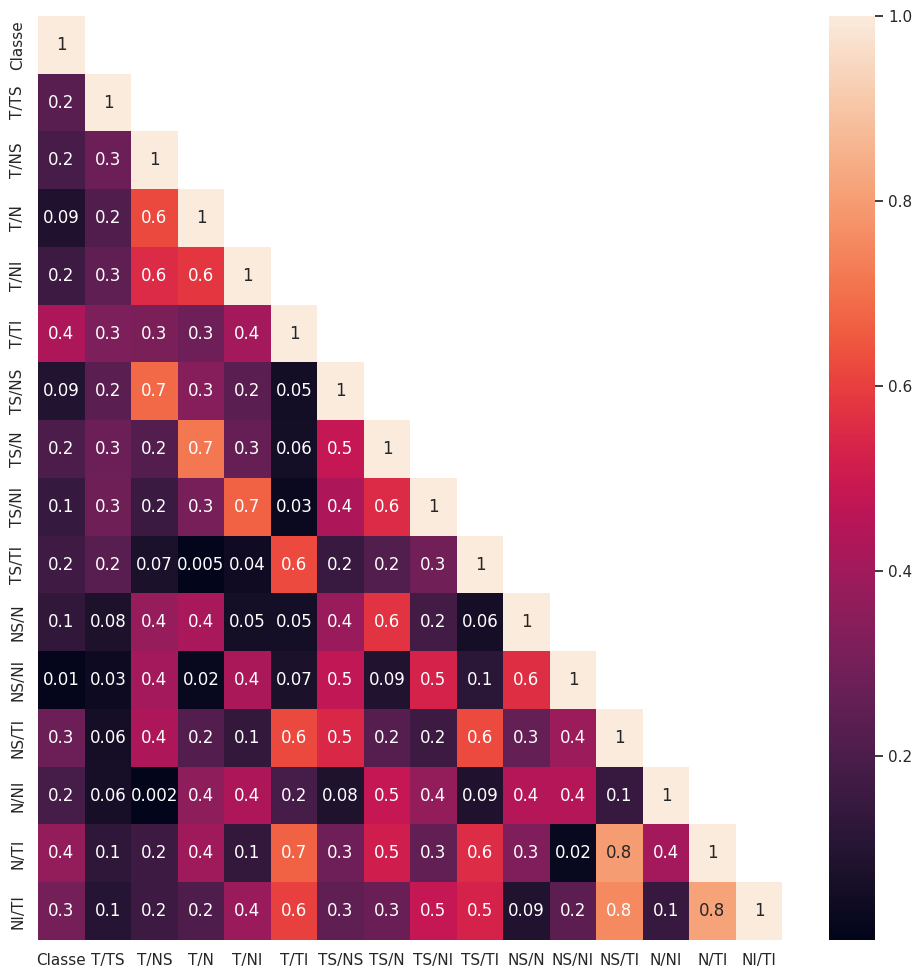
\includegraphics[width=0.98\textwidth]{./img/corr_eng_f.png}
        \small{Fonte: Elaborado pelo autor.}
    \end{figure}

    A fígura~\ref{fig:engcorr} mostra a correlação das características criadas sintéticamente com a
    operação de razão. Podemos observar que
    as duas características que mais apresentam correlação com a classe (presença ou ausência de
    glaucoma) são: N/TI e T/TI\@. No cápitulo de resultados~\ref{results}, mais especificamente na seção de
    explicabilidade~\ref{sec:resultexp}, será averiguado se alguma destas características criadas foram importantes para
    o modelo.


    \chapter{Experimentos}\label{experiments}

    \section{Setup}
    Todos os experimentos foram executados em uma máquina com processador i7\-3770, 16
    gigabytes\footnote{Gigabyte (símbolo Gbyte, GB, G) é uma unidade de medida de informação, segundo o
    Sistema Internacional de Unidades \- S.I., que equivale a um bilhão (milhar de milhões) de bytes,
    ou seja, 1.000.000.000 bytes, ou ainda $10^{9}$ bytes} de
    ram e uma placa de video Nvidia RTX-3060 com 12 gigabytes de memória.

    Dentre os \textit{softwares}\footnote{Software é um termo técnico que foi traduzido para
    a língua portuguesa como suporte lógico
    e trata-se de uma sequência de instruções a serem seguidas e/ou executadas, na manipulação, redirecionamento ou modificação de um dado (informação) ou acontecimento.} utilizados estão as seguintes bibliotecas de
    Python\footnote{https://www.python.org/}: \textit{Pytorch}\footnote{https://pytorch.org/},
    \textit{Seaborn}\footnote{https://seaborn.pydata.org/}, \textit{SHAP}~\footnote{https://github.com/slundberg/shap} e
    \textit{Pandas}\footnote{https://pandas.pydata.org/}. Para execução das análises foi utilizada o
    \textit{Jupyter Notebook}\footnote{https://jupyter.org/}.


    \section{\textit{Fine-Tunning}}\label{sec:fineextraction}

    Os modelos que foram utilizados como \textit{backbones} são modelos que já foram treinados
    anteriormente com algum conjunto de dados de imagens, não necessariamente similar ao desse
    projeto.
    Dado isso,  existem três formas mais utilizadas para fazer o treinamento para cada modelo. A
    primeira, conhecida como \textit{scratch}, é um treinamento em que inicializamos os modelos com
    parâmetros de forma randômica e em seguida aplicamos nossos dados para que o modelo consiga aprender padrões
    do zero. O segundo método é conhecido como \textit{feature extract} que é quando
    utilizamos os modelos \textit{backbones}, com os pesos já treinados em um grupo de dados
    diferente, e queremos utilizar deste pesos e apenas adicionar uma nova camada (normalmente a
    última) que será adaptada
    para o nosso conjunto de dados. Neste caso, todo o treinamento será feito apenas nessa última
    camada adicionada, enquanto os pesos das redes neurais pretreinadas serão congelados. E existe
    um terceiro modo, conhecido como \textit{fine-tunning}, onde iremos treinar todo o modelo
    pretreinado com os dados desejados.

    Dos métodos citado acima, as literaturas apontam que o \textit{fine-tunning} consegue desempenhar
    melhor em grande maioria das tarefas. Primeiro, para o caso de treinamento utilizando o
    método \textit{scratch} é necessário um volume grande dados, já que redes neurais convolucionais
    possuem um número grande pesos ou parâmetros a serem treinados. Desta forma, quanto mais
    parâmetros mais dados são necessários para generalizar. Para o segundo caso de \textit{feature
    extraction} o modelo preserva os pesos em que foi treinado originalmente e então é treinado
    somente a camada nova adicionada com o conjutno de dados que queremos utilizar.
    No entanto, o modelo não consegue se especializar já que teremos algumas poucas adaptações dos pesos para
    tarefa que queremos aplicar, limitado em pequenas mudanças nesta última camada adicionada.
    Enquanto no terceiro caso, o \textit{fine-tunning}, conseguimos aproveitar a complexidade do
    modelo treinado em um conjunto de dados mais volumoso e heterogeneo e ao mesmo tempo conseguimos
    adaptar este modelo para a tarefa que desejamos \citep{DBLP:journals/corr/LiH16e,
    Girshick2014RichFH, Azizpour2016FactorsOT, Agrawal2014AnalyzingTP, Yosinski2014HowTA}.

    Logo, para este projeto, iremos utilizar somente o \textit{fine-tunning} como método de
    treinamento dos modelos.

    % \section{\textit{Hiperparameter Tunning: Optuna}}
    % \label{sec:optuna}

    % O Optuna é uma ferramenta de busca de hiperparâmetros para os modelos de forma inteligênte. As
    % testagens são automaticamente selecionadas utilizando os históricos de tentativa. Desta forma é
    % possível que a ferramenta já elimine, com evidências empíricas, de testar hiperparâmetros não
    % promissores. Com isto, temos uma convergência mais rápida do modelo.

    % Agregado à isso, a ferramenta é fácil de configurar e também é escalável, podendo ser executado
    % múltiplas tentativas em paralelo. Para que essas tentativas conversem entre si e não haja
    % repetição de hiperparâmetros já testado, a ferramenta utiliza um banco de dados para armazenar
    % toda as tentativas.

    % O Optuna utiliza diferentes estratégias e algoritmos para testagem de parâmetros. É possível
    % configurar a ferramenta para utilizar a otimização bayesiana \citep{bayesian} ou algoritmos
    % evolucionários \citep{evolutionary} para a busca de hiperparâmetros (\textit{Sampling Strategy)}. A segunda estratégia foca
    % em no método de \textit{Early Stopping}~\ref{sec:trainval} citada anteriormente com o objetivo
    % de eliminar tentativas não promissoras (\textit{Pruning Strategy}).


    % Com isto, ao final da modelagem, foi utilizada a ferramenta para buscar melhor desempenho dos
    % modelos. Na seção de resultados, será possível visualizar os hiperparâmetros explorados e
    % tentados pela ferramenta e os resultados obtidos por ao final do processo.


    \section{\textit{Learning Rate Decay}}\label{sec:decay}

    \textit{Learning Rate Decay} (LRD) é uma tećnica de treinamento de rede neurais. O modelo começa com taxa
    de aprendizagem   e vai decaindo essa taxa múltiplas vezes durante o treinamento.
    Dessa maneira, o modelo começa atualizando os pesos mais rapidamente até que se chega em um
    certo ponto onde é necessário trabalhar com números menores e atualizações mais lentas. Dado isto, a taxa de
    aprendizagem do modelo irá diminuir, diminuindo os valores de atualização dos parâmetros e
    consequetemente atingindo valores melhores em desempenho.

    Os seguinte trabalhos trazem um pouco do benefício do \textit{learning rate decay} \citep{lrpaper1,
    lrpaper2}. A imagem na figura~\ref{fig:lrdecay} mostra que em um certo momento os modelos ResNet-18 e
    ResNet-34 chegam em um platô onde o erro do modelo não decrementa. A partir deste momento, a
    taxa de aprendizagem é subtraída por um valor e em seguida, o modelo volta a melhorar
    sua desempenho. Com isso, o modelo com taxas menores consegue fazer ajustes mais finos, ou em
    outras palavras, dar passos menores.

    \begin{figure}
        \centering
        \caption{\textit{Learning Rate Decay} aplicado a modelos visuais.}
        \label{fig:lrdecay}
        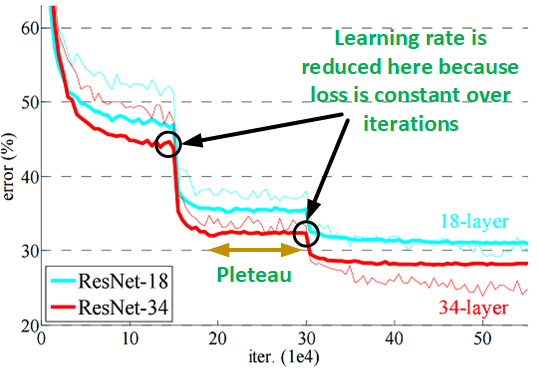
\includegraphics[width=0.98\textwidth]{./img/learning_decay.png}
            \small{Fonte: \href{https://towardsdatascience.com/the-subtle-art-of-fixing-and-modifying-learning-rate-f1e22b537303}{Towards Data Science}}
    \end{figure}


    \section{Experimentação}

    Os experimentos foram divididos em etapas, da seguinte forma:

    \begin{itemize}
        \item Primeiro foram testados os seguintes modelos utilizando diferente configurações:
            Mobile,RegNet (X e Y), ShuffleNet,
            EfficientNet, Inception-V3, ResNet, e ViT. Cada um dos modelos citados anteriormente foram testados com 4 diferente
            otimizadores (Adam, RAdam, SGD, Ranger) de parâmetros e 4 valores de taxa de
            aprendizagem (0.01, 0.001, 0.0001, 0.0005). Ao final desta etapa, foram selecionado os
            melhores modelos de acordo com a métrica AUC para a próxima etapa. Além disso, esta
            etapa fornceu o melhor momento para aplicar o \textit{Learning Rate Decay} e o \textit{Early
            Stopping} para ser utilizado nas próximas etapas.
        \item Em seguida os melhores K modelos são testado, utilizando decaimento de taxa de
            aprendizagem e \textit{Early Stopping} utilizando validação cruzada.
        \item Em seguida, os melhores M modelos dos K foram selecionados e é aplicado o
            \textit{RandAugment}~\ref{sec:aug} para trazer mais diversidade para os dados de treino e
            verificar o impacto, em questão de desempenho, do \textit{Data Augmentation}
    \end{itemize}


    A partir do segundo passo, todo os testes foram feitos utilizando a metodologia validação
    cruzada citada anteriormente com parâmetro igual 5, ou seja, dividido em 5 grupos. A decisão de
    aplicar somente a partir do segundo passo é o número exponencial de modelos a serem treinados
    caso fosse aplicado desde primeiro passo. Em todas as etapas, o número de épocas padrão é 100.

    Uma \textbf{observação} importante é sobre a separação dos dados de treino e teste. A separação
    deve aconteceu a nível de paciente e não de olho, para que assim, um paciente não tenha dados de
    um olho no treino e dados de outro olho no teste. Desta modo, evitou-se que houvesse vazamento de
    dados e o modelo demostre uma desempenho irreal.

    \begin{table}[h]
    \centering
    \setlength{\extrarowheight}{0pt}
    \addtolength{\extrarowheight}{\aboverulesep}
    \addtolength{\extrarowheight}{\belowrulesep}
    \setlength{\aboverulesep}{0pt}
    \setlength{\belowrulesep}{0pt}
    \caption{Versões dos modelos visuais utilizados como Backbones  e o total de parâmetros de cada um. O modelo ViT é o que possui maior número de parâmetros, aproximadamente 86 milhões, enquanto o modelo Shuffle possui somente 2.5 milhões. }
    \label{tab:bversions}
    \resizebox{\textwidth}{!}{%
    \begin{tabular}{!{\vrule width \heavyrulewidth}>{\hspace{0pt}}m{0.51\textwidth}!{\vrule width \heavyrulewidth}>{\hspace{0pt}}m{0.363\textwidth}!{\vrule width \heavyrulewidth}}
    \toprule
    \textit{\textbf{Backbone}} & \textbf{Parâmetros} \\
    \toprule
    \rowcolor[rgb]{0.761,0.761,0.761} RegNet800MFX & 6.586.329 \\
    \toprule
    RegNet800MFY & 5.648.297 \\
    \toprule
    \rowcolor[rgb]{0.761,0.761,0.761} RegNet1.6GFX & 8.279.048 \\
    \toprule
    RegNet1.6GFY & 10.314.319 \\
    \toprule
    \rowcolor[rgb]{0.761,0.761,0.761} RegNet3.2GFX & 14.288.561 \\
    \toprule
    RegNet3.2GFY & 17.824.851 \\
    \toprule
    \rowcolor[rgb]{0.761,0.761,0.761} MobileV3Large & 4.203.313 \\
    \toprule
    Resnet50 & 23.510.081 \\
    \toprule
    \rowcolor[rgb]{0.761,0.761,0.761} EfficientNetb0 & 4.008.829 \\
    \toprule
    ShuffleNetV1X1.5 & 2.479.649 \\
    \toprule
    \rowcolor[rgb]{0.761,0.761,0.761} VitBase16\_224 & 85.799.425 \\
    \toprule
    InceptionV3 & 24.346.082 \\
    \bottomrule
    \end{tabular}}
        \small{Fonte: Elaborado pelo autor.}
    \end{table}


   A tabela~\ref{tab:bversions} possui a versão e o total de par&aemtros dos modelos citados na seção~\ref{sec:model}
   implementados dentro da biblitoeca Pytorch\footnote{Biblioteca Python de aprendizado de máquina}.


    %% Contudo é possível ainda melhorar o modelo utizando um otimizador bayesiano tipo optuna. esta biblioteca fornece múltiplos algoritmos para seleção do melhor modelo
    %% Com isso é possível fazer testes rápidos. Testando mais possibilidades é possível convergir mais rápido, já que teremos mais trials por minuto. Logo, com iterações
    %% é possível chegar no mínimo local. Completude de features, podemos usar o ilca.


    \chapter{Resultados}\label{results}

    Neste cápitulo iremos apresentar os resultados. Na primeira seção iremos apresentar uma visão
    geral dos modelos quanto a desempenho relação a nossa métrica principal, AUC~\ref{sec:metrics}.
    Além disso, pela gráfico de perda (loss) teremos um ponto ideal para cada um
    dos modelos quanto a hora de aplicarmos a técnica de \textit{Learning Rate Decay}~\ref{sec:decay}
    para conseguirmos uma desempenho ainda melhor nas próximas etapas.

    \section{Desempenho Geral}\label{sec:general}

    A fígura~\ref{fig:geralauc} mostra como foi a desempenho geral dos modelos. Nota-se que os
    modelos utilizando os dados de OCT atingiram melhores resultados do que aqueles que não usa,
    tanto para modelos utilizando uma imagem quanto para modelos utilizando duas imagens. A
    distruição do modelo que não utiliza OCT é menos esparsa quanto aus resultados no teste, com
    exceção do ViT.
    Enquanto, os modelos utilizando OCT possuem uma variabilidade maior quanto ao desempenho. Este
    compartamento é encontrado quanto nos modelos utilizando uma ou duas imagens.

    \begin{figure}[ht]
        \centering
        \caption{Avaliação geral dos modelos divididos em uso de duas imagens e presença das métricas do
        OCT. O gráfico violino mostra a distruição dos valores máximos atingindos por cada
        \textit{backbone}}
        \label{fig:geralauc}
        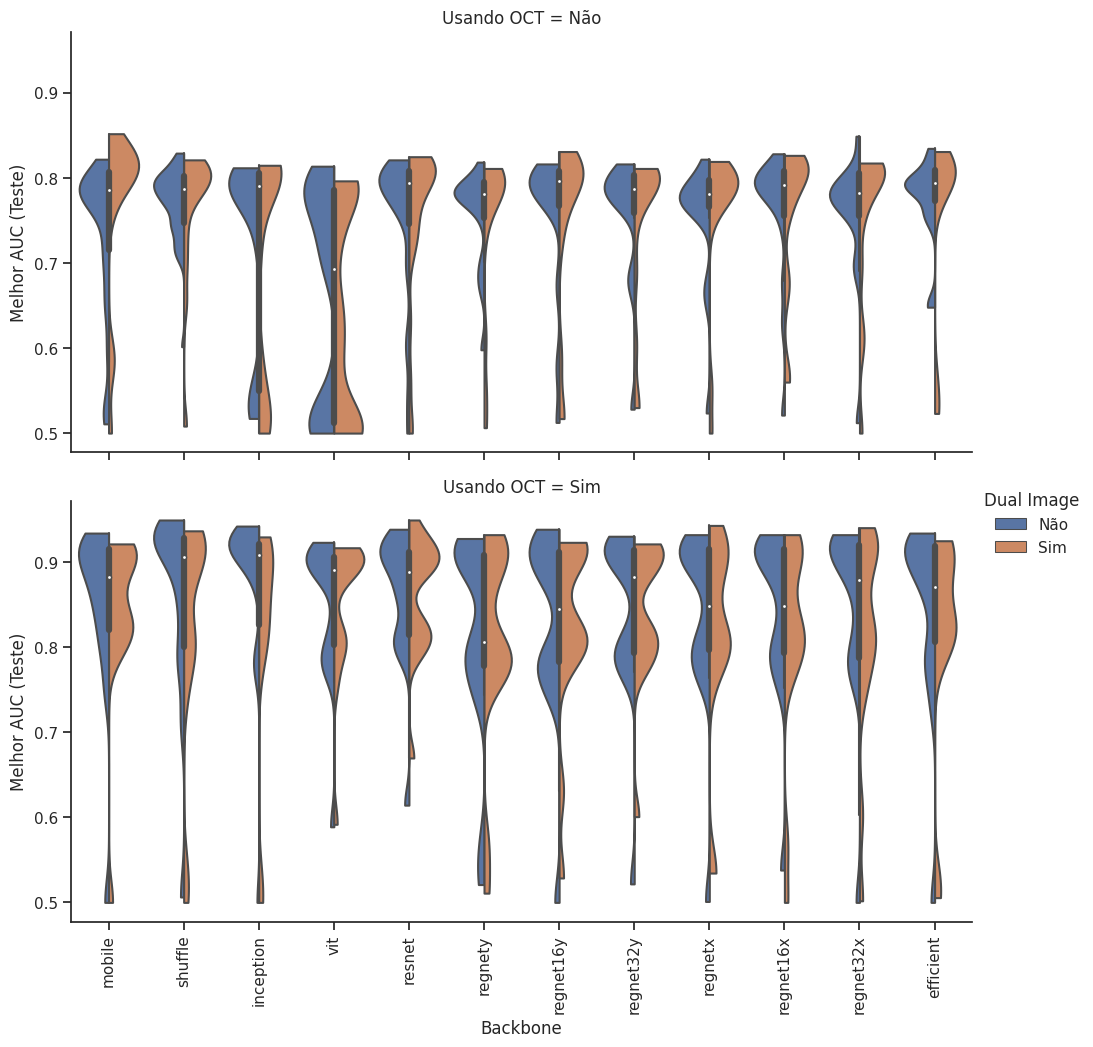
\includegraphics[width=0.98\textwidth]{./img/melhor_auc_lr_learning.png}
        \small{Fonte: Elaborado pelo autor.}
    \end{figure}


    O gráfico~\ref{fig:scatter} usa a média da AUC no treinamento e o valor máximo atingido para
    comparar os modelos. É perceptível que os modelos estão distribuídos de forma uniforme no
    gráfico quando comparamos os grupos. Os modelos RegNetY e RegNetX não sobreasem quanto ao
    desempenho quando comparados juntos. Além disso, existe uma relação direta entre a média de AUC
    no treinamento e o valor máximo que essa atinge durante todo o processo, com raros casos de
    discrepância.

    \begin{figure}[H]
        \centering
        \caption{Comparação das estatisticas da métrica AUC. O eixo y é o melhor resultado do modelo
        durante todas as épocas, enquanto o eixo x é a média do modelo durante o treinamento.}
        \label{fig:scatter}
        \begin{subfigure}[ht]{0.48\textwidth}
            \centering
            \caption{Comparação entre grupo de modelos RegNet e todos os outros.}
            \label{fig:scatter1}
            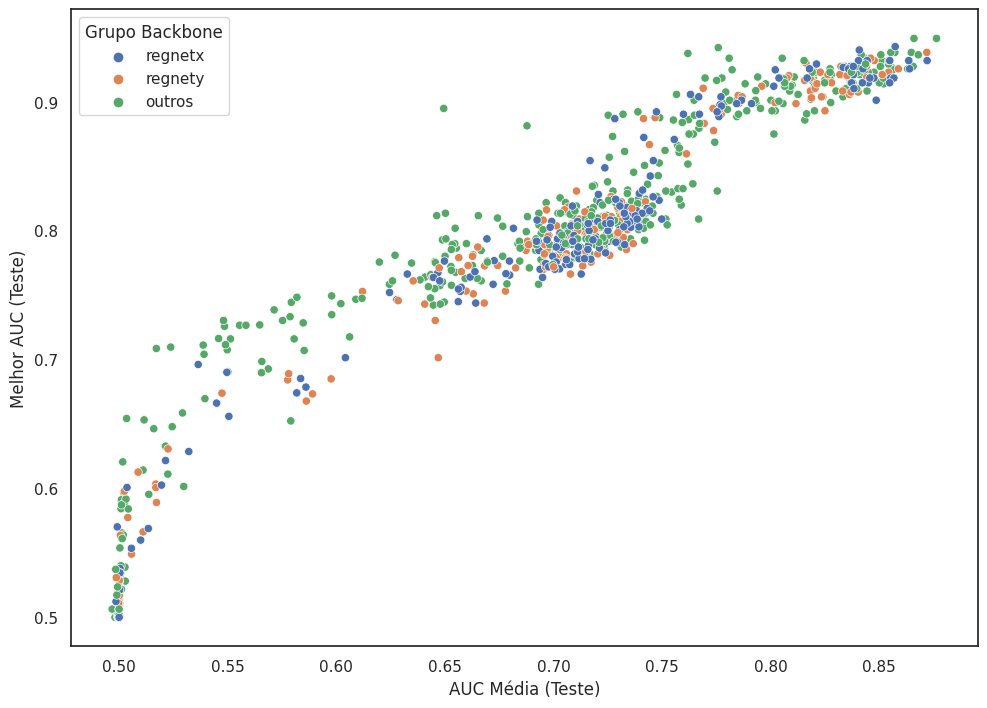
\includegraphics[width=0.98\textwidth]{./img/scatter1.png}
        \end{subfigure}
        \hfill
        \begin{subfigure}[ht]{0.48\textwidth}
            \centering
            \caption{Comparação entre os modelos RegNet por si.}
            \label{fig:scatter2}
            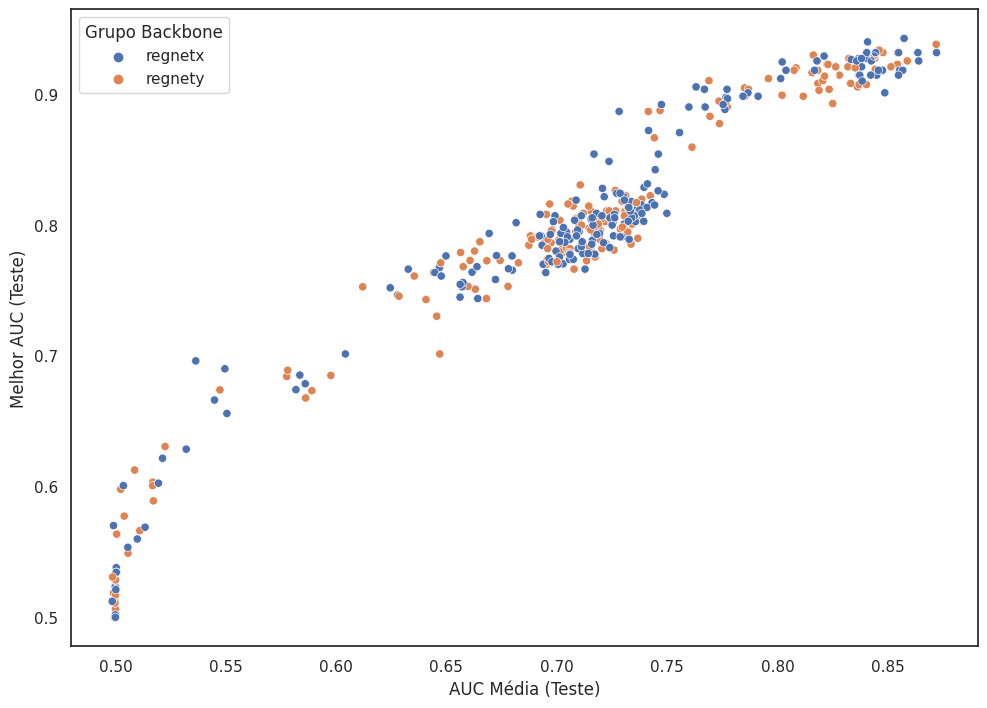
\includegraphics[width=0.98\textwidth]{./img/scatter2.png}
        \end{subfigure}
        \small{Fonte: Elaborado pelo autor.}
    \end{figure}


    As tabelas~\ref{tab:aucbackbone} e~\ref{tab:aucdualoct} sumarizam todas as execuções dos
    \textit{backbone} em todas as arquiteturas discutidas~\ref{fig:arqui}. Quanto a máxima AUC
    atingida pelos modelos, todos estes tiveram valor próximo de 0.93. Quanto as arquiteturas
    testadas, podemos obsevar que a presença do OCT traz benefícios para o modelo, aumentando até em
    em 12\% o desempenho dos modelos. No entanto, não houve melhora dos modelos quando utilizamos
    uma ou duas imagens na arquitetura. Dito isso, foi limitado daqui pra frente o uso de modelos
    utilizando somente uma imagem de entrada.

    \begin{table}[ht]
    \centering
    \caption{Tabela contendo os resultados quanto a métrica AUC separado por backbone. Todos os
    modelos parecem possuir resultados próximos.}
    \setlength{\extrarowheight}{0pt}
    \addtolength{\extrarowheight}{\aboverulesep}
    \addtolength{\extrarowheight}{\belowrulesep}
    \setlength{\aboverulesep}{0pt}
    \setlength{\belowrulesep}{0pt}
    \resizebox{\linewidth}{!}{%
    \label{tab:aucbackbone}
    \begin{tabular}{>{\hspace{0pt}}m{0.175\linewidth}>{\hspace{0pt}}m{0.087\linewidth}>{\hspace{0pt}}m{0.087\linewidth}>{\hspace{0pt}}m{0.106\linewidth}>{\hspace{0pt}}m{0.087\linewidth}>{\hspace{0pt}}m{0.075\linewidth}>{\hspace{0pt}}m{0.087\linewidth}>{\hspace{0pt}}m{0.106\linewidth}>{\hspace{0pt}}m{0.087\linewidth}}
    \toprule
    Backbone & \multicolumn{4}{>{\hspace{0pt}}m{0.367\linewidth}}{Melhor AUC} & \multicolumn{4}{>{\hspace{0pt}}m{0.355\linewidth}}{AUC Média} \\
    \cmidrule(lr){2-5}\cmidrule(lr){6-9}
    & min & max & mean & std & min & max & mean & std \\
    \midrule
    efficient & 0.5 & 0.93 & 0.8 & 0.11 & 0.5 & 0.85 & 0.72 & 0.1 \\
    \rowcolor[rgb]{0.761,0.761,0.761} inception & 0.5 & 0.94 & 0.79 & 0.14 & 0.5 & 0.86 & 0.7 & 0.12 \\
    mobile & 0.5 & 0.93 & 0.79 & 0.11 & 0.5 & 0.84 & 0.69 & 0.1 \\
    \rowcolor[rgb]{0.761,0.761,0.761} regnet16x & 0.5 & 0.93 & 0.79 & 0.1 & 0.5 & 0.86 & 0.71 & 0.09 \\
    regnet16y & 0.5 & 0.94 & 0.79 & 0.11 & 0.5 & 0.87 & 0.71 & 0.09 \\
    \rowcolor[rgb]{0.761,0.761,0.761} regnet32x & 0.5 & 0.94 & 0.79 & 0.11 & 0.5 & 0.87 & 0.71 & 0.1 \\
    regnet32y & 0.52 & 0.93 & 0.8 & 0.1 & 0.5 & 0.86 & 0.71 & 0.09 \\
    \rowcolor[rgb]{0.761,0.761,0.761} regnetx & 0.5 & 0.94 & 0.79 & 0.11 & 0.5 & 0.86 & 0.71 & 0.09 \\
    regnety & 0.51 & 0.93 & 0.78 & 0.11 & 0.5 & 0.85 & 0.7 & 0.09 \\
    \rowcolor[rgb]{0.761,0.761,0.761} resnet & 0.5 & 0.95 & 0.79 & 0.1 & 0.5 & 0.87 & 0.7 & 0.1 \\
    shuffle & 0.5 & 0.95 & 0.8 & 0.09 & 0.5 & 0.88 & 0.7 & 0.1 \\
    \rowcolor[rgb]{0.761,0.761,0.761} vit & 0.5 & 0.92 & 0.75 & 0.15 & 0.5 & 0.85 & 0.67 & 0.12 \\
    \bottomrule
    \end{tabular}}
    \small{Fonte: Elaborado pelo autor.}
    \end{table}

    \begin{table}[ht]
    \centering
        \caption{Tabela contendo os resultados separado por dois grupos: OCT e Dual Image. A tabela
        mostra que Dual Image não trás benefícios, enquanto a utilização do exame OCT agrega performance
        aos resultados}
    \setlength{\extrarowheight}{0pt}
    \addtolength{\extrarowheight}{\aboverulesep}
    \addtolength{\extrarowheight}{\belowrulesep}
    \setlength{\aboverulesep}{0pt}
    \setlength{\belowrulesep}{0pt}
    \resizebox{\linewidth}{!}{%
    \label{tab:aucdualoct}
    \begin{tabular}{>{\hspace{0pt}}m{0.16\linewidth}>{\hspace{0pt}}m{0.181\linewidth}>{\hspace{0pt}}m{0.06\linewidth}>{\hspace{0pt}}m{0.069\linewidth}>{\hspace{0pt}}m{0.085\linewidth}>{\hspace{0pt}}m{0.069\linewidth}>{\hspace{0pt}}m{0.06\linewidth}>{\hspace{0pt}}m{0.069\linewidth}>{\hspace{0pt}}m{0.085\linewidth}>{\hspace{0pt}}m{0.069\linewidth}}
    \toprule
    \multirow{2}{0.16\linewidth}{\hspace{0pt}Dual Image} & \multirow{2}{0.181\linewidth}{\hspace{0pt}Usando OCT} & \multicolumn{4}{>{\hspace{0pt}}m{0.283\linewidth}}{Melhor AUC} & \multicolumn{4}{>{\hspace{0pt}}m{0.283\linewidth}}{AUC Média} \\
    \cmidrule{3-6}\cmidrule(lr){7-10}
    &  & min & max & mean & std & min & max & mean & std \\
    \midrule
    Não & Não & 0.5 & 0.85 & 0.75 & 0.08 & 0.5 & 0.74 & 0.66 & 0.07 \\
    \rowcolor[rgb]{0.761,0.761,0.761} Não & Sim & 0.5 & 0.95 & 0.85 & 0.1 & 0.5 & 0.88 & 0.75 & 0.1 \\
    Sim & Não & 0.5 & 0.85 & 0.74 & 0.11 & 0.5 & 0.77 & 0.66 & 0.09 \\
    \rowcolor[rgb]{0.761,0.761,0.761} Sim & Sim & 0.5 & 0.95 & 0.83 & 0.11 & 0.5 & 0.87 & 0.74 & 0.1 \\
    \bottomrule
    \end{tabular}}
        \small{Fonte: Elaborado pelo autor.}
    \end{table}

    A distribuiçãodos desempenhos apresentados na fígura~\ref{fig:distarqui} mostra uma seperação clara
    entre OCT e não. No entanto, como citado anteriormente não há diferença do modelo utilizando uma
    ou duas imagens. Dado isso, foi selecionado os melhores 5\%, baseado na AUC, dos modelos usando uma image e uma
    imagem mais os dados de OCT. Para seleção foi utilizado o percentil\footnote{Em estatística
    descritiva, os percentis são medidas que dividem a amostra (por ordem crescente dos dados) em
    100 partes, cada uma com uma percentagem de dados aproximadamente igual. O k-ésimo percentil
    $P_{k}$ é o valor x ($x_{k}$) que corresponde à frequência cumulativa de N.k/100, onde N é o tamanho
    amostral.} 95 e todos os modelos abaixo desse valor foram filtrados. Ao final, restaram um total
    28 modelos.

    \begin{figure}[H]
        \centering
        \caption{Distribuição dos desempenhos separado por arquiteturas de modelos}
        \label{fig:distarqui}
        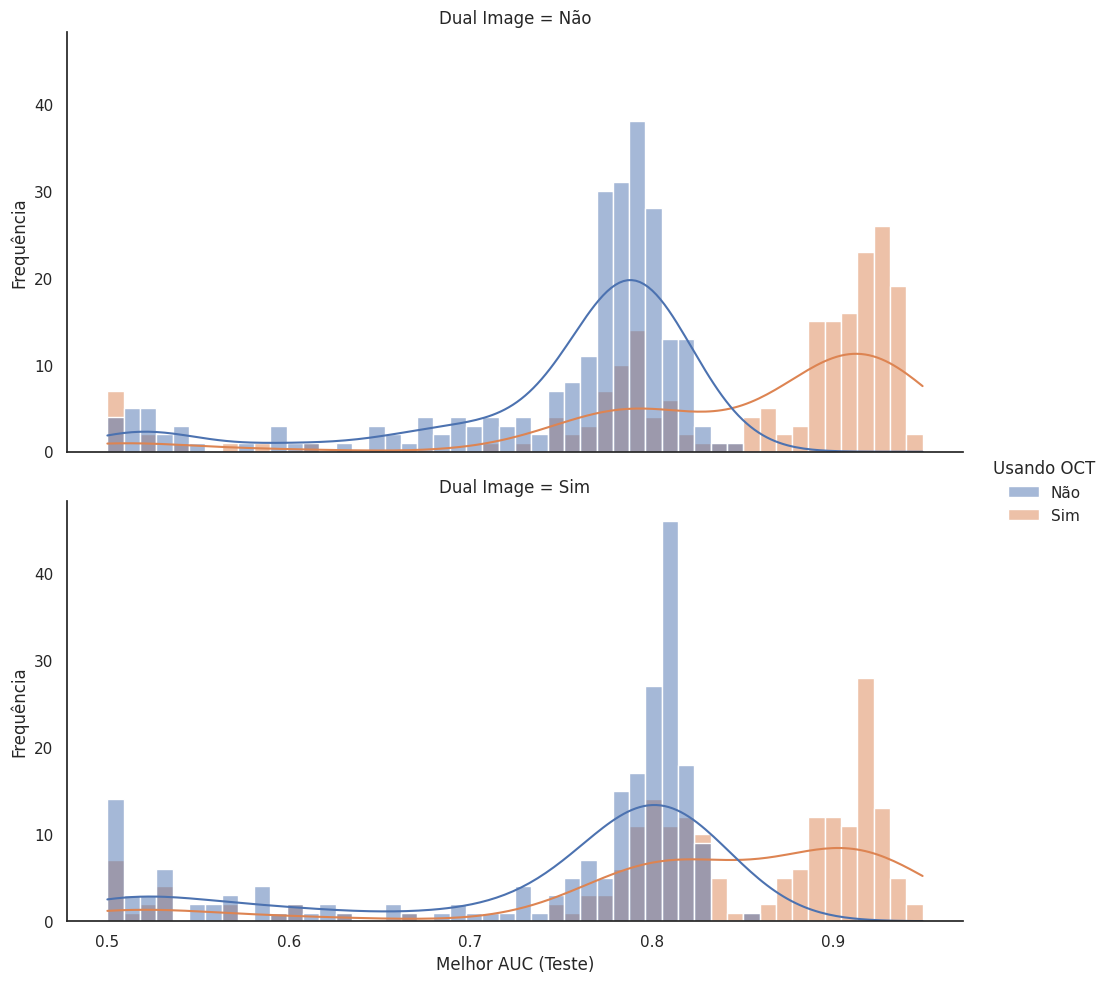
\includegraphics[width=0.98\textwidth]{./img/distarqui.png}
        \small{Fonte: Elaborado pelo autor.}
    \end{figure}



    E por útlimo, o gráfico~\ref{fig:lossepochs} da função de custo durante o treinamento. O gráfico mostrau uma média
    global de todos os modelos treinados com um intervalo de confiança de 0.95. O gráfico mostra que
    a partir da época 30 o modelo não consegue ter uma melhoria no seu desempenho. Portanto, é nesse
    momento que aplicamos o \textit{Early Stopping} e o \textit{Learning Rate Decay} para próxima fase de
    experimentos utilizando validação cruzada.


    \begin{figure}[H]
        \centering
        \caption{Comportamento da função de custo durante as épocas de treinamento. O gráfico mostra
        um valor médio e um intervalo de confiança de 0.95}
        \label{fig:lossepochs}
        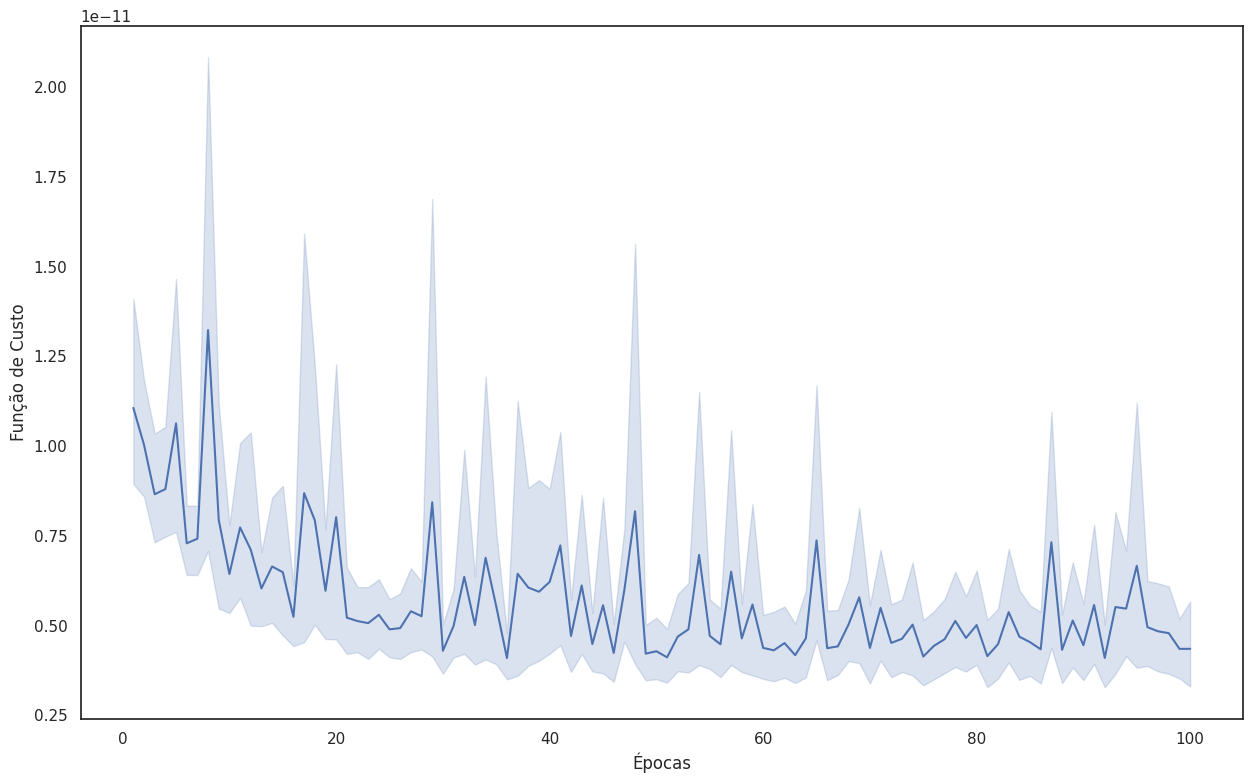
\includegraphics[width=0.98\textwidth]{./img/lossepochs.png}
        \small{Fonte: Elaborado pelo autor.}
    \end{figure}

    \section{Validação Cruzada e \textit{Learning Rate Decay}}

    Nesta seção iremos avaliar os melhores modelos selecionados na etapa anterior e verificar seu
    desempenho utilizando a validção cruzada \citep{cross-val}. O total de grupos para experimento
    foi igual 5, ou seja, cada configuração de hiperparâmetros gerou 5 modelos diferentes,
    totalizando 140 modelos, com seus respectivos desempenhos. Além disso, foram será ilustrada uma
    comparação entre a utilização do \textit{Learning Rate Decay} utilizando validação cruzada.

    A seguir~\ref{tab:summarytop}, a tabela contendo os hiperparâmetros e os \textit{backbones} dos modelos testados. O
    campo \textbf{Usando OCT} se refere a usar os dados do exame OCT junto com o modelo de imagem.
    Dentre os melhores modelos, a família de modelos RegNet aparece em 16 dos 18 melhores modelos.
    Isso mostra que o RegNet além ter um desempenho bom, é também um modelo a ser escolhido na
    tentativa de executar uma tarefa de visão computacional. As várias versões do modelo que
    aparece, mostra que este modelo é flexível e pode ser utilizado em diferentes contextos, com
    diferentes disponibilidades de recursos.

    %\begin{table}
\centering
\caption{Resultados comparando a utilização do Learning Decay(ld) e sua ausência nas métricas de AUC, especificidade(sp) e sensitividade(sn)}
\label{tab:results_ld}
\begin{tabular}{c|c|c|c|c|c|c|c|c|c|c|c|c|}
\toprule
{} &   optim &     lr &  output\_tab &  val\_best\_auc &  val\_best\_auc\_ld &  avg\_best\_auc\_val &  avg\_best\_auc\_val\_ld &  idx\_max\_sp\_val &  idx\_max\_sp\_val\_ld &  idx\_max\_sn\_val &  idx\_max\_sn\_val\_ld &  idx\_avg\_sp\_val &  idx\_avg\_sp\_val\_ld &  idx\_avg\_sn\_val &  idx\_avg\_sn\_val\_ld \\
\textbf{backbone } &         &        &             &               &                  &                   &                      &                 &                    &                 &                    &                 &                    &                 &                    \\
\midrule
\textbf{regnet16x} &   radam &  0.001 &         0.0 &         0.792 &            0.899 &               NaN &                0.818 &             NaN &              0.929 &             NaN &              0.882 &             NaN &              0.913 &             NaN &              0.722 \\
\textbf{regnet16x} &   radam &  0.000 &         0.0 &         0.828 &            0.888 &               NaN &                0.801 &           0.874 &              0.924 &           0.783 &              0.853 &             NaN &              0.906 &             NaN &              0.695 \\
\textbf{inception} &  ranger &  0.000 &         0.0 &         0.810 &            0.859 &               NaN &                0.781 &           0.946 &              0.951 &           0.674 &              0.794 &             NaN &              0.891 &             NaN &              0.670 \\
\textbf{inception} &     sgd &  0.010 &         0.0 &         0.812 &            0.811 &               NaN &                0.756 &           0.928 &              0.962 &           0.696 &              0.818 &             NaN &              0.880 &             NaN &              0.633 \\
\textbf{inception} &  ranger &  0.001 &         0.0 &         0.812 &            0.899 &               NaN &                0.795 &           0.928 &              0.935 &           0.696 &              0.882 &             NaN &              0.923 &             NaN &              0.666 \\
\textbf{regnet32x} &   radam &  0.001 &         0.0 &         0.849 &            0.882 &               NaN &                0.805 &           0.937 &              0.947 &           0.761 &              0.882 &             NaN &              0.905 &             NaN &              0.706 \\
\textbf{resnet   } &    adam &  0.010 &         5.0 &         0.939 &            0.943 &               NaN &                0.673 &           0.964 &              1.000 &           0.913 &              0.912 &             NaN &              0.993 &             NaN &              0.353 \\
\textbf{resnet   } &  ranger &  0.010 &         5.0 &         0.937 &            0.961 &               NaN &                0.836 &           0.982 &              0.991 &           0.891 &              0.941 &             NaN &              0.969 &             NaN &              0.702 \\
\textbf{regnet32y} &    adam &  0.000 &         5.0 &         0.930 &            0.945 &               NaN &                0.897 &           0.991 &              0.982 &           0.870 &              0.955 &             NaN &              0.951 &             NaN &              0.842 \\
\textbf{regnet32y} &    adam &  0.010 &         5.0 &         0.926 &            0.937 &               NaN &                0.745 &           0.982 &              1.000 &           0.870 &              0.882 &             NaN &              0.989 &             NaN &              0.501 \\
\textbf{mobile   } &   radam &  0.010 &         5.0 &         0.926 &            0.928 &               NaN &                0.892 &           0.982 &              1.000 &           0.870 &              0.941 &             NaN &              0.946 &             NaN &              0.839 \\
\textbf{shuffle  } &  ranger &  0.010 &         5.0 &         0.949 &            0.981 &               NaN &                0.935 &           0.964 &              0.975 &           0.935 &              1.000 &             NaN &              0.963 &             NaN &              0.907 \\
\textbf{shuffle  } &   radam &  0.001 &         5.0 &         0.934 &            0.926 &               NaN &                0.826 &           0.955 &              0.953 &           0.913 &              0.971 &             NaN &              0.924 &             NaN &              0.728 \\
\textbf{shuffle  } &  ranger &  0.001 &         5.0 &         0.932 &            0.903 &               NaN &                0.795 &           0.973 &              0.971 &           0.891 &              0.882 &             NaN &              0.927 &             NaN &              0.663 \\
\textbf{shuffle  } &   radam &  0.010 &         5.0 &         0.932 &            0.989 &               NaN &                0.937 &           0.973 &              1.000 &           0.891 &              0.977 &             NaN &              0.976 &             NaN &              0.897 \\
\textbf{regnetx  } &    adam &  0.010 &         5.0 &         0.926 &            0.984 &               NaN &                0.934 &           0.982 &              0.991 &           0.870 &              0.977 &             NaN &              0.968 &             NaN &              0.900 \\
\textbf{regnetx  } &    adam &  0.001 &         5.0 &         0.915 &            0.986 &               NaN &                0.914 &           0.982 &              0.973 &           0.848 &              1.000 &             NaN &              0.967 &             NaN &              0.860 \\
\textbf{regnetx  } &   radam &  0.010 &         5.0 &         0.932 &            0.986 &               NaN &                0.933 &           0.973 &              1.000 &           0.891 &              1.000 &             NaN &              0.968 &             NaN &              0.897 \\
\textbf{regnet16y} &  ranger &  0.010 &         5.0 &         0.932 &            0.973 &               NaN &                0.890 &           0.973 &              0.991 &           0.891 &              0.955 &             NaN &              0.947 &             NaN &              0.833 \\
\textbf{regnet16y} &    adam &  0.010 &         5.0 &         0.939 &            0.939 &               NaN &                0.663 &           0.964 &              1.000 &           0.913 &              0.912 &             NaN &              0.991 &             NaN &              0.335 \\
\textbf{regnet16y} &   radam &  0.010 &         5.0 &         0.934 &            0.989 &               NaN &                0.933 &           0.955 &              1.000 &           0.913 &              0.977 &             NaN &              0.973 &             NaN &              0.893 \\
\textbf{efficient} &    adam &  0.010 &         5.0 &         0.928 &            0.979 &               NaN &                0.847 &           0.964 &              0.992 &           0.891 &              0.977 &             NaN &              0.960 &             NaN &              0.734 \\
\textbf{regnet32x} &   radam &  0.010 &         5.0 &         0.926 &            0.986 &               NaN &                0.940 &           0.982 &              0.991 &           0.870 &              1.000 &             NaN &              0.958 &             NaN &              0.922 \\
\textbf{regnet32x} &   radam &  0.001 &         5.0 &         0.926 &            0.865 &               NaN &                0.801 &           0.982 &              0.943 &           0.870 &              0.824 &             NaN &              0.892 &             NaN &              0.711 \\
\textbf{regnet32x} &  ranger &  0.010 &         5.0 &         0.932 &            0.951 &               NaN &                0.899 &           0.973 &              0.991 &           0.891 &              0.977 &             NaN &              0.957 &             NaN &              0.841 \\
\textbf{regnet32x} &    adam &  0.010 &         5.0 &         0.932 &            0.986 &               NaN &                0.940 &           0.973 &              1.000 &           0.891 &              1.000 &             NaN &              0.973 &             NaN &              0.907 \\
\textbf{regnet16x} &   radam &  0.010 &         5.0 &         0.932 &            0.991 &               NaN &                0.927 &           0.973 &              0.990 &           0.891 &              1.000 &             NaN &              0.963 &             NaN &              0.891 \\
\textbf{inception} &  ranger &  0.010 &         5.0 &         0.929 &            0.979 &               NaN &                0.909 &           0.946 &              0.990 &           0.913 &              0.977 &             NaN &              0.969 &             NaN &              0.850 \\
\bottomrule
\end{tabular}
\end{table}


    A fígura~\ref{fig:crosscompare} mostra a distribuição do desempenho dos modelos testados. O
    \textit{Learning Rate Decay} trouxe uma melhora significativa para as duas arquiteturas. Apesar de
    ter aumentando a variabilidade da AUC, a técnica trouxe benefícios positivos quanto a métrica. O
    salto maior foi para a arquitetura de modelos utilizando somente imagem.

    \begin{figure}\label{fig:crosscompare}
        \centering
        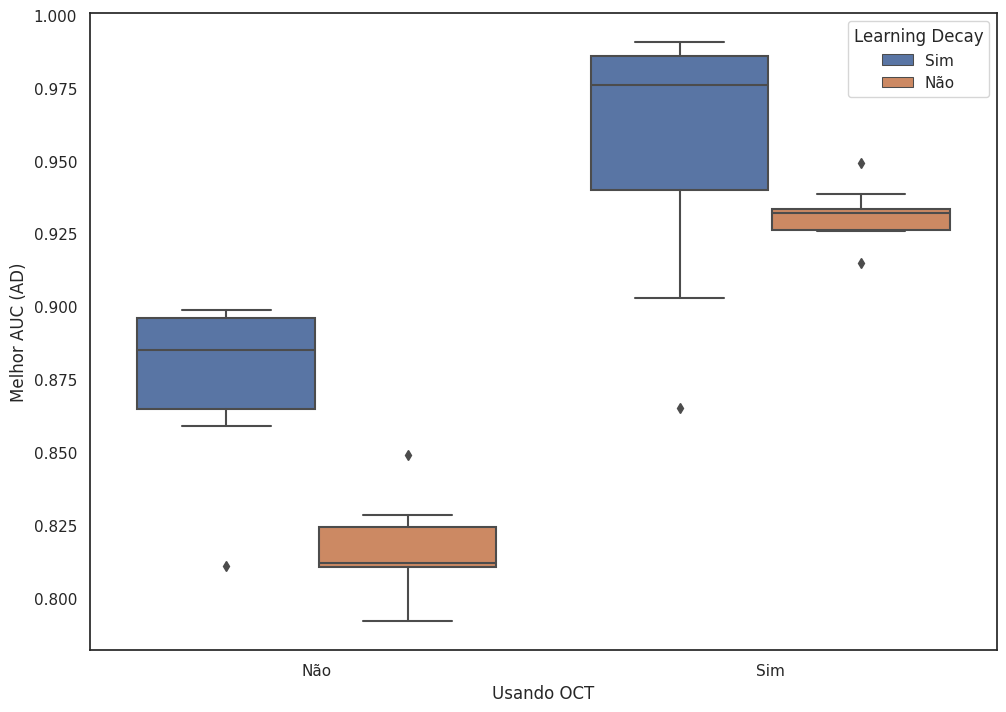
\includegraphics[width=0.6\textwidth]{./img/cross_compare.png}
        \caption{Comparação do uso do \textit{Learning Rate Decay} nos melhores modelos. Os melhores
        modelos da etapa anterior foram re-executados utilizando validação cruzada para uma
        comparação justa.}
    \end{figure}


    Quanto ao uso de memória e tempo de inferência, é possível observar que o modelos RegNets
    possuem  tempo de inferência menor quando comparado aos modelos mais complexos ou até
    mesmo com os mais simples, como é no caso no ShuffleNet. Isto proporciona flexibilidade
    para que o modelo RegNet possa ser utilizado em diferente contextos que é necessário uma
    resposta rápida, como por exemplo quadros de um video ou em algum sistema nuvem que recebe
    milhares de requisições ao mesmo tempo. Quanto ao uso de memória, os modelos RegNets apresentam
    várias versões com diferentes uso de recursos computacionais. Variando de 1600 megabytes até
    4182, o modelo consegue apresentar desempenho mesmo no modelo com menor uso, até mesmo que o
    mobile (1662), ultrapassando
    modelos mais caros como por exemplo inception (4722). Com tudo, os modelos acima ainda consegue
    oferecer desempenhos satisfatórios para o caso de uso de uma imagem e de image somados ao exame
    OCT.


    \subsection{\textit{RandAugment}}

    Dado os resultados da seção anterior, foram selecionados 3 modelos para aplicar \textit{data
    augmentation}. Um dos hiperparâmetros do \textit{RandAugument} é o nome de operações sequenciais
    em uma foto. Por esse motivo, foram testados diferentes valores para este hiperparâmetro: 1, 2,
    3 e 4. Nesta etapa também foi utilizada validação cruzada para avaliar o modelo.

    A tabela acima mostra que o \textit{RandAugment} não trouxe melhoras significativas para o
    modelo. O resultado foi inverso do esperado, diminuindo o desempenho dos modelos, tanto na
    métrica de AUC quanto nas métricas de especificidade(sp) e sensitividade(sn).


    \section{Explicabilidade}\label{sec:resultexp}

    Nesta seção iremos trazer a explicabilidade dos melhores modelos. O objetivo é entender a
    interação do modelos com os dados, tanto de imagen quanto os tabulares, para então seja possível
    entender o porque da decisão do modelo. Iremos avaliar tanto as imagens do fundo do olho e
    verificar quais foram as partes cruciais das imagens, quanto os valores tabelados conténdo as
    medições e as características criadas e descritas na seção~\ref{sec:engineering}.

    \subsection{Compara arquitetura 1 olho e dois olhos}

    \subsection{1 olho e 1 olho + tabular}

    \subsection{Importância média das features tab}

    \subsection{Caso positivo e negativo}


    \chapter{Conclusão}
    \label{conclusion}

    Ao final do projeto foi perceptível como os modelos RegNet conseguem ser flexíveis em todos os
    contextos. O modelo apresentou desempenho ótimo em diferentes arquitetruas de modelos. Dentre os
    melhores modelos, o modelo RegNet é o que mais aparece com suas diferentes versões quanto ao uso
    de memória e ao número de parâmetros. Contudo, a escolha do modelo RegNet proporciona uma maior
    probabilidade de se obter um desempenho na detecção do glaucoma utilizando imagens do fundo do
    olho e do exame OCT. Além disso, o modelo também apresenta um custo computacional (memória)
    menor em vários casos e ao mesmo tempo sobresaindo em desempenho, inclusive quanto ao tempo de
    inferência. Dado isso, é possível que o modelo RegNet seja uma escolha sólida em tarefas de
    visão computacional que exige eficiência, eficácia e flexibilidade ao mesmo tempo.

    O \textit{Rand Augmentation} não mostrou benefícios quanto ao desempenho do modelo ou ao menos
    quanto sua variabilidade. No entanto, apesar de não ter sido um sucesso neste projeto, este tipo
    de técnia não deve descartada já que aqui não foram testados todos as combinações de
    hiperparâmetros e modelagens possíveis devido ao limitante computacional. Por outra lado, a
    técnica de \textit{Learning Rate Decay} apresentou benefícios para os modelos, aumentando seu
    desempenho quanto a métrica AUC.

    %% Referências
    \bibliographystyle{plain}
    \bibliography{referencias}

\end{document}

